\documentclass[twoside]{book}

% Packages required by doxygen
\usepackage{fixltx2e}
\usepackage{calc}
\usepackage{doxygen}
\usepackage[export]{adjustbox} % also loads graphicx
\usepackage{graphicx}
\usepackage[utf8]{inputenc}
\usepackage{makeidx}
\usepackage{multicol}
\usepackage{multirow}
\PassOptionsToPackage{warn}{textcomp}
\usepackage{textcomp}
\usepackage[nointegrals]{wasysym}
\usepackage[table]{xcolor}

% Font selection
\usepackage[T1]{fontenc}
\usepackage[scaled=.90]{helvet}
\usepackage{courier}
\usepackage{amssymb}
\usepackage{sectsty}
\renewcommand{\familydefault}{\sfdefault}
\allsectionsfont{%
  \fontseries{bc}\selectfont%
  \color{darkgray}%
}
\renewcommand{\DoxyLabelFont}{%
  \fontseries{bc}\selectfont%
  \color{darkgray}%
}
\newcommand{\+}{\discretionary{\mbox{\scriptsize$\hookleftarrow$}}{}{}}

% Page & text layout
\usepackage{geometry}
\geometry{%
  a4paper,%
  top=2.5cm,%
  bottom=2.5cm,%
  left=2.5cm,%
  right=2.5cm%
}
\tolerance=750
\hfuzz=15pt
\hbadness=750
\setlength{\emergencystretch}{15pt}
\setlength{\parindent}{0cm}
\setlength{\parskip}{3ex plus 2ex minus 2ex}
\makeatletter
\renewcommand{\paragraph}{%
  \@startsection{paragraph}{4}{0ex}{-1.0ex}{1.0ex}{%
    \normalfont\normalsize\bfseries\SS@parafont%
  }%
}
\renewcommand{\subparagraph}{%
  \@startsection{subparagraph}{5}{0ex}{-1.0ex}{1.0ex}{%
    \normalfont\normalsize\bfseries\SS@subparafont%
  }%
}
\makeatother

% Headers & footers
\usepackage{fancyhdr}
\pagestyle{fancyplain}
\fancyhead[LE]{\fancyplain{}{\bfseries\thepage}}
\fancyhead[CE]{\fancyplain{}{}}
\fancyhead[RE]{\fancyplain{}{\bfseries\leftmark}}
\fancyhead[LO]{\fancyplain{}{\bfseries\rightmark}}
\fancyhead[CO]{\fancyplain{}{}}
\fancyhead[RO]{\fancyplain{}{\bfseries\thepage}}
\fancyfoot[LE]{\fancyplain{}{}}
\fancyfoot[CE]{\fancyplain{}{}}
\fancyfoot[RE]{\fancyplain{}{\bfseries\scriptsize Generated by Doxygen }}
\fancyfoot[LO]{\fancyplain{}{\bfseries\scriptsize Generated by Doxygen }}
\fancyfoot[CO]{\fancyplain{}{}}
\fancyfoot[RO]{\fancyplain{}{}}
\renewcommand{\footrulewidth}{0.4pt}
\renewcommand{\chaptermark}[1]{%
  \markboth{#1}{}%
}
\renewcommand{\sectionmark}[1]{%
  \markright{\thesection\ #1}%
}

% Indices & bibliography
\usepackage{natbib}
\usepackage[titles]{tocloft}
\setcounter{tocdepth}{3}
\setcounter{secnumdepth}{5}
\makeindex

% Hyperlinks (required, but should be loaded last)
\usepackage{ifpdf}
\ifpdf
  \usepackage[pdftex,pagebackref=true]{hyperref}
\else
  \usepackage[ps2pdf,pagebackref=true]{hyperref}
\fi
\hypersetup{%
  colorlinks=true,%
  linkcolor=blue,%
  citecolor=blue,%
  unicode%
}

% Custom commands
\newcommand{\clearemptydoublepage}{%
  \newpage{\pagestyle{empty}\cleardoublepage}%
}

\usepackage{caption}
\captionsetup{labelsep=space,justification=centering,font={bf},singlelinecheck=off,skip=4pt,position=top}

%===== C O N T E N T S =====

\begin{document}

% Titlepage & ToC
\hypersetup{pageanchor=false,
             bookmarksnumbered=true,
             pdfencoding=unicode
            }
\pagenumbering{alph}
\begin{titlepage}
\vspace*{7cm}
\begin{center}%
{\Large E\+SM }\\
\vspace*{1cm}
{\large Generated by Doxygen 1.8.14}\\
\end{center}
\end{titlepage}
\clearemptydoublepage
\pagenumbering{roman}
\tableofcontents
\clearemptydoublepage
\pagenumbering{arabic}
\hypersetup{pageanchor=true}

%--- Begin generated contents ---
\chapter{Hierarchical Index}
\section{Class Hierarchy}
This inheritance list is sorted roughly, but not completely, alphabetically\+:\begin{DoxyCompactList}
\item \contentsline{section}{modules.\+center.\+Center}{\pageref{classmodules_1_1center_1_1_center}}{}
\item \contentsline{section}{system.\+Database}{\pageref{classsystem_1_1_database}}{}
\item Exception\begin{DoxyCompactList}
\item \contentsline{section}{system.\+exceptions.\+Data\+Card\+Exception}{\pageref{classsystem_1_1exceptions_1_1_data_card_exception}}{}
\item \contentsline{section}{system.\+exceptions.\+Person\+Doesnt\+Exist\+Exception}{\pageref{classsystem_1_1exceptions_1_1_person_doesnt_exist_exception}}{}
\item \contentsline{section}{system.\+exceptions.\+Surname\+Exception}{\pageref{classsystem_1_1exceptions_1_1_surname_exception}}{}
\end{DoxyCompactList}
\item \contentsline{section}{Testing.\+Main}{\pageref{class_testing_1_1_main}}{}
\item \contentsline{section}{gui.\+views.\+View}{\pageref{classgui_1_1views_1_1_view}}{}
\begin{DoxyCompactList}
\item \contentsline{section}{gui.\+views.\+Bank\+View}{\pageref{classgui_1_1views_1_1_bank_view}}{}
\item \contentsline{section}{gui.\+views.\+Center\+View}{\pageref{classgui_1_1views_1_1_center_view}}{}
\item \contentsline{section}{gui.\+views.\+Company\+View}{\pageref{classgui_1_1views_1_1_company_view}}{}
\item \contentsline{section}{gui.\+views.\+Login\+View}{\pageref{classgui_1_1views_1_1_login_view}}{}
\end{DoxyCompactList}
\item J\+Frame\begin{DoxyCompactList}
\item \contentsline{section}{gui.\+Window}{\pageref{classgui_1_1_window}}{}
\end{DoxyCompactList}
\item Serializable\begin{DoxyCompactList}
\item \contentsline{section}{modules.\+bank.\+Bank}{\pageref{classmodules_1_1bank_1_1_bank}}{}
\item \contentsline{section}{modules.\+bank.\+Card}{\pageref{classmodules_1_1bank_1_1_card}}{}
\begin{DoxyCompactList}
\item \contentsline{section}{modules.\+bank.\+Bank\+Card}{\pageref{classmodules_1_1bank_1_1_bank_card}}{}
\item \contentsline{section}{modules.\+bank.\+Credit\+Card}{\pageref{classmodules_1_1bank_1_1_credit_card}}{}
\item \contentsline{section}{modules.\+bank.\+Debit\+Card}{\pageref{classmodules_1_1bank_1_1_debit_card}}{}
\end{DoxyCompactList}
\item \contentsline{section}{modules.\+center.\+Transaction}{\pageref{classmodules_1_1center_1_1_transaction}}{}
\item \contentsline{section}{modules.\+center.\+User}{\pageref{classmodules_1_1center_1_1_user}}{}
\item \contentsline{section}{modules.\+Client}{\pageref{classmodules_1_1_client}}{}
\item \contentsline{section}{modules.\+company.\+Company}{\pageref{classmodules_1_1company_1_1_company}}{}
\begin{DoxyCompactList}
\item \contentsline{section}{modules.\+company.\+A\+T\+M\+Company}{\pageref{classmodules_1_1company_1_1_a_t_m_company}}{}
\item \contentsline{section}{modules.\+company.\+Service\+Company}{\pageref{classmodules_1_1company_1_1_service_company}}{}
\item \contentsline{section}{modules.\+company.\+Shop\+Company}{\pageref{classmodules_1_1company_1_1_shop_company}}{}
\item \contentsline{section}{modules.\+company.\+Transport\+Company}{\pageref{classmodules_1_1company_1_1_transport_company}}{}
\end{DoxyCompactList}
\end{DoxyCompactList}
\end{DoxyCompactList}

\chapter{Class Index}
\section{Class List}
Here are the classes, structs, unions and interfaces with brief descriptions\+:\begin{DoxyCompactList}
\item\contentsline{section}{\mbox{\hyperlink{classmodules_1_1company_1_1_a_t_m_company}{modules.\+company.\+A\+T\+M\+Company}} }{\pageref{classmodules_1_1company_1_1_a_t_m_company}}{}
\item\contentsline{section}{\mbox{\hyperlink{classmodules_1_1bank_1_1_bank}{modules.\+bank.\+Bank}} }{\pageref{classmodules_1_1bank_1_1_bank}}{}
\item\contentsline{section}{\mbox{\hyperlink{classmodules_1_1bank_1_1_bank_card}{modules.\+bank.\+Bank\+Card}} }{\pageref{classmodules_1_1bank_1_1_bank_card}}{}
\item\contentsline{section}{\mbox{\hyperlink{classgui_1_1views_1_1_bank_view}{gui.\+views.\+Bank\+View}} }{\pageref{classgui_1_1views_1_1_bank_view}}{}
\item\contentsline{section}{\mbox{\hyperlink{classmodules_1_1bank_1_1_card}{modules.\+bank.\+Card}} }{\pageref{classmodules_1_1bank_1_1_card}}{}
\item\contentsline{section}{\mbox{\hyperlink{classmodules_1_1center_1_1_center}{modules.\+center.\+Center}} }{\pageref{classmodules_1_1center_1_1_center}}{}
\item\contentsline{section}{\mbox{\hyperlink{classgui_1_1views_1_1_center_view}{gui.\+views.\+Center\+View}} }{\pageref{classgui_1_1views_1_1_center_view}}{}
\item\contentsline{section}{\mbox{\hyperlink{classmodules_1_1_client}{modules.\+Client}} }{\pageref{classmodules_1_1_client}}{}
\item\contentsline{section}{\mbox{\hyperlink{classmodules_1_1company_1_1_company}{modules.\+company.\+Company}} }{\pageref{classmodules_1_1company_1_1_company}}{}
\item\contentsline{section}{\mbox{\hyperlink{classgui_1_1views_1_1_company_view}{gui.\+views.\+Company\+View}} }{\pageref{classgui_1_1views_1_1_company_view}}{}
\item\contentsline{section}{\mbox{\hyperlink{classmodules_1_1bank_1_1_credit_card}{modules.\+bank.\+Credit\+Card}} }{\pageref{classmodules_1_1bank_1_1_credit_card}}{}
\item\contentsline{section}{\mbox{\hyperlink{classsystem_1_1_database}{system.\+Database}} }{\pageref{classsystem_1_1_database}}{}
\item\contentsline{section}{\mbox{\hyperlink{classsystem_1_1exceptions_1_1_data_card_exception}{system.\+exceptions.\+Data\+Card\+Exception}} }{\pageref{classsystem_1_1exceptions_1_1_data_card_exception}}{}
\item\contentsline{section}{\mbox{\hyperlink{classmodules_1_1bank_1_1_debit_card}{modules.\+bank.\+Debit\+Card}} }{\pageref{classmodules_1_1bank_1_1_debit_card}}{}
\item\contentsline{section}{\mbox{\hyperlink{classgui_1_1views_1_1_login_view}{gui.\+views.\+Login\+View}} }{\pageref{classgui_1_1views_1_1_login_view}}{}
\item\contentsline{section}{\mbox{\hyperlink{class_testing_1_1_main}{Testing.\+Main}} }{\pageref{class_testing_1_1_main}}{}
\item\contentsline{section}{\mbox{\hyperlink{classsystem_1_1exceptions_1_1_person_doesnt_exist_exception}{system.\+exceptions.\+Person\+Doesnt\+Exist\+Exception}} }{\pageref{classsystem_1_1exceptions_1_1_person_doesnt_exist_exception}}{}
\item\contentsline{section}{\mbox{\hyperlink{classmodules_1_1company_1_1_service_company}{modules.\+company.\+Service\+Company}} }{\pageref{classmodules_1_1company_1_1_service_company}}{}
\item\contentsline{section}{\mbox{\hyperlink{classmodules_1_1company_1_1_shop_company}{modules.\+company.\+Shop\+Company}} }{\pageref{classmodules_1_1company_1_1_shop_company}}{}
\item\contentsline{section}{\mbox{\hyperlink{classsystem_1_1exceptions_1_1_surname_exception}{system.\+exceptions.\+Surname\+Exception}} }{\pageref{classsystem_1_1exceptions_1_1_surname_exception}}{}
\item\contentsline{section}{\mbox{\hyperlink{classmodules_1_1center_1_1_transaction}{modules.\+center.\+Transaction}} }{\pageref{classmodules_1_1center_1_1_transaction}}{}
\item\contentsline{section}{\mbox{\hyperlink{classmodules_1_1company_1_1_transport_company}{modules.\+company.\+Transport\+Company}} }{\pageref{classmodules_1_1company_1_1_transport_company}}{}
\item\contentsline{section}{\mbox{\hyperlink{classmodules_1_1center_1_1_user}{modules.\+center.\+User}} }{\pageref{classmodules_1_1center_1_1_user}}{}
\item\contentsline{section}{\mbox{\hyperlink{classgui_1_1views_1_1_view}{gui.\+views.\+View}} }{\pageref{classgui_1_1views_1_1_view}}{}
\item\contentsline{section}{\mbox{\hyperlink{classgui_1_1_window}{gui.\+Window}} }{\pageref{classgui_1_1_window}}{}
\end{DoxyCompactList}

\chapter{Class Documentation}
\hypertarget{classmodules_1_1company_1_1_a_t_m_company}{}\section{modules.\+company.\+A\+T\+M\+Company Class Reference}
\label{classmodules_1_1company_1_1_a_t_m_company}\index{modules.\+company.\+A\+T\+M\+Company@{modules.\+company.\+A\+T\+M\+Company}}
Inheritance diagram for modules.\+company.\+A\+T\+M\+Company\+:\begin{figure}[H]
\begin{center}
\leavevmode
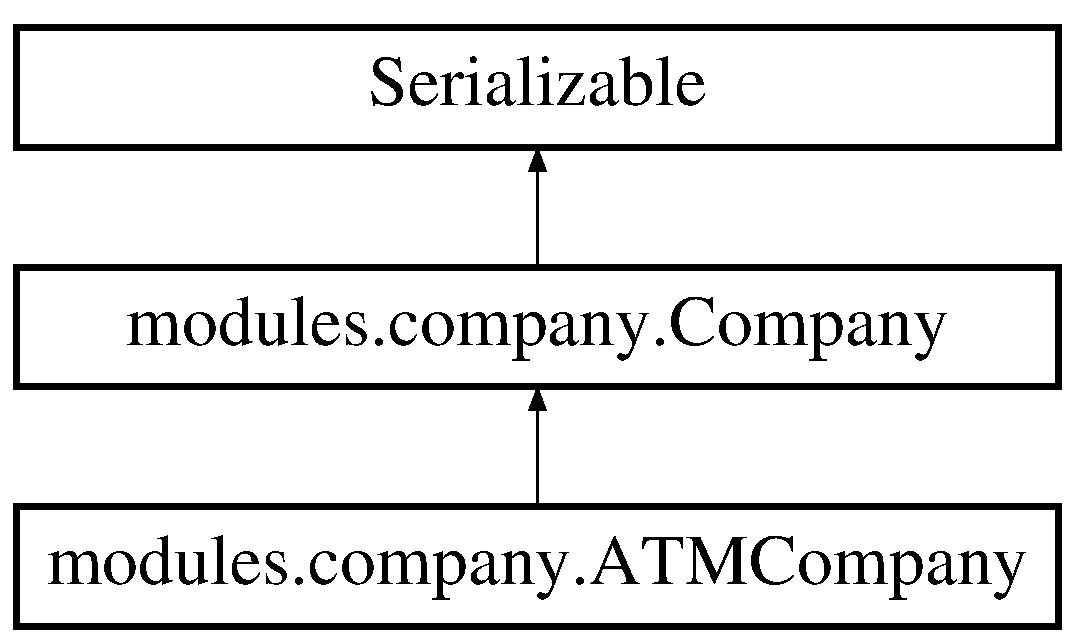
\includegraphics[height=3.000000cm]{classmodules_1_1company_1_1_a_t_m_company}
\end{center}
\end{figure}
\subsection*{Public Member Functions}
\begin{DoxyCompactItemize}
\item 
\mbox{\hyperlink{classmodules_1_1company_1_1_a_t_m_company_a0b29105d696d20573f178b27f3960451}{A\+T\+M\+Company}} (String name)
\end{DoxyCompactItemize}
\subsection*{Additional Inherited Members}


\subsection{Detailed Description}
Another type of center client \begin{DoxyAuthor}{Author}
Micha� Fi�o�czuk 
\end{DoxyAuthor}


\subsection{Constructor \& Destructor Documentation}
\mbox{\Hypertarget{classmodules_1_1company_1_1_a_t_m_company_a0b29105d696d20573f178b27f3960451}\label{classmodules_1_1company_1_1_a_t_m_company_a0b29105d696d20573f178b27f3960451}} 
\index{modules\+::company\+::\+A\+T\+M\+Company@{modules\+::company\+::\+A\+T\+M\+Company}!A\+T\+M\+Company@{A\+T\+M\+Company}}
\index{A\+T\+M\+Company@{A\+T\+M\+Company}!modules\+::company\+::\+A\+T\+M\+Company@{modules\+::company\+::\+A\+T\+M\+Company}}
\subsubsection{\texorpdfstring{A\+T\+M\+Company()}{ATMCompany()}}
{\footnotesize\ttfamily modules.\+company.\+A\+T\+M\+Company.\+A\+T\+M\+Company (\begin{DoxyParamCaption}\item[{String}]{name }\end{DoxyParamCaption})\hspace{0.3cm}{\ttfamily [inline]}}

Standard way to create A\+TM \mbox{\hyperlink{classmodules_1_1company_1_1_company}{Company}} 
\begin{DoxyParams}{Parameters}
{\em id} & \\
\hline
{\em name} & \\
\hline
\end{DoxyParams}


The documentation for this class was generated from the following file\+:\begin{DoxyCompactItemize}
\item 
modules/company/A\+T\+M\+Company.\+java\end{DoxyCompactItemize}

\hypertarget{classmodules_1_1bank_1_1_bank}{}\section{modules.\+bank.\+Bank Class Reference}
\label{classmodules_1_1bank_1_1_bank}\index{modules.\+bank.\+Bank@{modules.\+bank.\+Bank}}
Inheritance diagram for modules.\+bank.\+Bank\+:\begin{figure}[H]
\begin{center}
\leavevmode
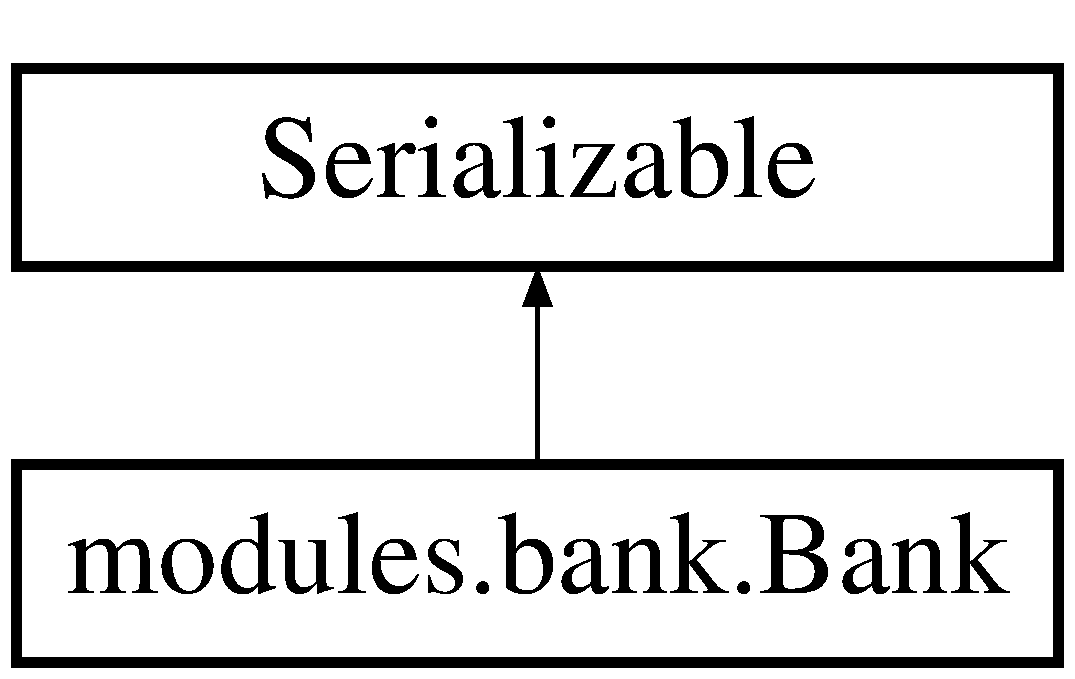
\includegraphics[height=2.000000cm]{classmodules_1_1bank_1_1_bank}
\end{center}
\end{figure}
\subsection*{Public Member Functions}
\begin{DoxyCompactItemize}
\item 
\mbox{\hyperlink{classmodules_1_1bank_1_1_bank_adab0c5144eabfff1ec68b17c85ccb82c}{Bank}} (String name)
\item 
void \mbox{\hyperlink{classmodules_1_1bank_1_1_bank_a09c003792c8c8db5c497a6b52219b0f7}{add\+Client}} (\mbox{\hyperlink{classmodules_1_1_client}{Client}} client)
\item 
void \mbox{\hyperlink{classmodules_1_1bank_1_1_bank_ae7ca045a74af810ef3a725d4caa675dc}{delete\+\_\+\+Client}} (String pesel)  throws Person\+Doesnt\+Exist\+Exception 
\item 
boolean \mbox{\hyperlink{classmodules_1_1bank_1_1_bank_ab1f1401b5f940afa992f956dcc14fe68}{check\+Transaction}} (\mbox{\hyperlink{classmodules_1_1center_1_1_transaction}{Transaction}} trans)
\item 
String \mbox{\hyperlink{classmodules_1_1bank_1_1_bank_a0eab8718f802478789bd6af09fe5830f}{get\+Name}} ()
\item 
void \mbox{\hyperlink{classmodules_1_1bank_1_1_bank_af1a426fe4526cbc9d5cefa289bd36856}{set\+Name}} (String name)
\item 
Array\+List$<$ \mbox{\hyperlink{classmodules_1_1_client}{Client}} $>$ \mbox{\hyperlink{classmodules_1_1bank_1_1_bank_ab883f59128823f976fbea30f363f1328}{get\+Clients}} ()
\item 
void \mbox{\hyperlink{classmodules_1_1bank_1_1_bank_afb7f67a0bc547c413df5f284af824a32}{set\+Clients}} (Array\+List$<$ \mbox{\hyperlink{classmodules_1_1_client}{Client}} $>$ clients)
\end{DoxyCompactItemize}


\subsection{Detailed Description}
Class represents specified \mbox{\hyperlink{classmodules_1_1bank_1_1_bank}{Bank}} object \begin{DoxyAuthor}{Author}
Micha� Fi�o�czuk 
\end{DoxyAuthor}
\begin{DoxyVersion}{Version}
0.\+5 
\end{DoxyVersion}


\subsection{Constructor \& Destructor Documentation}
\mbox{\Hypertarget{classmodules_1_1bank_1_1_bank_adab0c5144eabfff1ec68b17c85ccb82c}\label{classmodules_1_1bank_1_1_bank_adab0c5144eabfff1ec68b17c85ccb82c}} 
\index{modules\+::bank\+::\+Bank@{modules\+::bank\+::\+Bank}!Bank@{Bank}}
\index{Bank@{Bank}!modules\+::bank\+::\+Bank@{modules\+::bank\+::\+Bank}}
\subsubsection{\texorpdfstring{Bank()}{Bank()}}
{\footnotesize\ttfamily modules.\+bank.\+Bank.\+Bank (\begin{DoxyParamCaption}\item[{String}]{name }\end{DoxyParamCaption})\hspace{0.3cm}{\ttfamily [inline]}}

Standard \mbox{\hyperlink{classmodules_1_1bank_1_1_bank}{Bank}} constructor 
\begin{DoxyParams}{Parameters}
{\em name} & \\
\hline
\end{DoxyParams}

\begin{DoxyExceptions}{Exceptions}
{\em Data\+Card\+Exception} & \\
\hline
\end{DoxyExceptions}


\subsection{Member Function Documentation}
\mbox{\Hypertarget{classmodules_1_1bank_1_1_bank_a09c003792c8c8db5c497a6b52219b0f7}\label{classmodules_1_1bank_1_1_bank_a09c003792c8c8db5c497a6b52219b0f7}} 
\index{modules\+::bank\+::\+Bank@{modules\+::bank\+::\+Bank}!add\+Client@{add\+Client}}
\index{add\+Client@{add\+Client}!modules\+::bank\+::\+Bank@{modules\+::bank\+::\+Bank}}
\subsubsection{\texorpdfstring{add\+Client()}{addClient()}}
{\footnotesize\ttfamily void modules.\+bank.\+Bank.\+add\+Client (\begin{DoxyParamCaption}\item[{\mbox{\hyperlink{classmodules_1_1_client}{Client}}}]{client }\end{DoxyParamCaption})\hspace{0.3cm}{\ttfamily [inline]}}

Adds \mbox{\hyperlink{classmodules_1_1_client}{Client}} to local list 
\begin{DoxyParams}{Parameters}
{\em client} & represents Object \mbox{\hyperlink{classmodules_1_1_client}{Client}} \\
\hline
\end{DoxyParams}
\mbox{\Hypertarget{classmodules_1_1bank_1_1_bank_ab1f1401b5f940afa992f956dcc14fe68}\label{classmodules_1_1bank_1_1_bank_ab1f1401b5f940afa992f956dcc14fe68}} 
\index{modules\+::bank\+::\+Bank@{modules\+::bank\+::\+Bank}!check\+Transaction@{check\+Transaction}}
\index{check\+Transaction@{check\+Transaction}!modules\+::bank\+::\+Bank@{modules\+::bank\+::\+Bank}}
\subsubsection{\texorpdfstring{check\+Transaction()}{checkTransaction()}}
{\footnotesize\ttfamily boolean modules.\+bank.\+Bank.\+check\+Transaction (\begin{DoxyParamCaption}\item[{\mbox{\hyperlink{classmodules_1_1center_1_1_transaction}{Transaction}}}]{trans }\end{DoxyParamCaption})\hspace{0.3cm}{\ttfamily [inline]}}

Transaction service 
\begin{DoxyParams}{Parameters}
{\em trans} & Transaction -\/ object to execute \\
\hline
\end{DoxyParams}
\begin{DoxyReturn}{Returns}
boolean true -\/ if transaction is accepted, false -\/ if transaction is rejected 
\end{DoxyReturn}
\begin{DoxyAuthor}{Author}
Ernest Stachelski \& Micha� Fi�o�czuk 
\end{DoxyAuthor}
\mbox{\Hypertarget{classmodules_1_1bank_1_1_bank_ae7ca045a74af810ef3a725d4caa675dc}\label{classmodules_1_1bank_1_1_bank_ae7ca045a74af810ef3a725d4caa675dc}} 
\index{modules\+::bank\+::\+Bank@{modules\+::bank\+::\+Bank}!delete\+\_\+\+Client@{delete\+\_\+\+Client}}
\index{delete\+\_\+\+Client@{delete\+\_\+\+Client}!modules\+::bank\+::\+Bank@{modules\+::bank\+::\+Bank}}
\subsubsection{\texorpdfstring{delete\+\_\+\+Client()}{delete\_Client()}}
{\footnotesize\ttfamily void modules.\+bank.\+Bank.\+delete\+\_\+\+Client (\begin{DoxyParamCaption}\item[{String}]{pesel }\end{DoxyParamCaption}) throws \mbox{\hyperlink{classsystem_1_1exceptions_1_1_person_doesnt_exist_exception}{Person\+Doesnt\+Exist\+Exception}}\hspace{0.3cm}{\ttfamily [inline]}}

Deletes \mbox{\hyperlink{classmodules_1_1_client}{Client}} with specified P\+E\+S\+EL 
\begin{DoxyParams}{Parameters}
{\em pesel} & -\/ String represents clients P\+E\+S\+EL \\
\hline
\end{DoxyParams}

\begin{DoxyExceptions}{Exceptions}
{\em Person\+Doesnt\+Exist\+Exception} & \\
\hline
\end{DoxyExceptions}
\mbox{\Hypertarget{classmodules_1_1bank_1_1_bank_ab883f59128823f976fbea30f363f1328}\label{classmodules_1_1bank_1_1_bank_ab883f59128823f976fbea30f363f1328}} 
\index{modules\+::bank\+::\+Bank@{modules\+::bank\+::\+Bank}!get\+Clients@{get\+Clients}}
\index{get\+Clients@{get\+Clients}!modules\+::bank\+::\+Bank@{modules\+::bank\+::\+Bank}}
\subsubsection{\texorpdfstring{get\+Clients()}{getClients()}}
{\footnotesize\ttfamily Array\+List$<$\mbox{\hyperlink{classmodules_1_1_client}{Client}}$>$ modules.\+bank.\+Bank.\+get\+Clients (\begin{DoxyParamCaption}{ }\end{DoxyParamCaption})\hspace{0.3cm}{\ttfamily [inline]}}

Getter List of Clients \begin{DoxyReturn}{Returns}
Array\+List Clients 
\end{DoxyReturn}
\mbox{\Hypertarget{classmodules_1_1bank_1_1_bank_a0eab8718f802478789bd6af09fe5830f}\label{classmodules_1_1bank_1_1_bank_a0eab8718f802478789bd6af09fe5830f}} 
\index{modules\+::bank\+::\+Bank@{modules\+::bank\+::\+Bank}!get\+Name@{get\+Name}}
\index{get\+Name@{get\+Name}!modules\+::bank\+::\+Bank@{modules\+::bank\+::\+Bank}}
\subsubsection{\texorpdfstring{get\+Name()}{getName()}}
{\footnotesize\ttfamily String modules.\+bank.\+Bank.\+get\+Name (\begin{DoxyParamCaption}{ }\end{DoxyParamCaption})\hspace{0.3cm}{\ttfamily [inline]}}

Getter \mbox{\hyperlink{classmodules_1_1bank_1_1_bank}{Bank}} Name \begin{DoxyReturn}{Returns}
String name 
\end{DoxyReturn}
\mbox{\Hypertarget{classmodules_1_1bank_1_1_bank_afb7f67a0bc547c413df5f284af824a32}\label{classmodules_1_1bank_1_1_bank_afb7f67a0bc547c413df5f284af824a32}} 
\index{modules\+::bank\+::\+Bank@{modules\+::bank\+::\+Bank}!set\+Clients@{set\+Clients}}
\index{set\+Clients@{set\+Clients}!modules\+::bank\+::\+Bank@{modules\+::bank\+::\+Bank}}
\subsubsection{\texorpdfstring{set\+Clients()}{setClients()}}
{\footnotesize\ttfamily void modules.\+bank.\+Bank.\+set\+Clients (\begin{DoxyParamCaption}\item[{Array\+List$<$ \mbox{\hyperlink{classmodules_1_1_client}{Client}} $>$}]{clients }\end{DoxyParamCaption})\hspace{0.3cm}{\ttfamily [inline]}}

Setter List of Clients 
\begin{DoxyParams}{Parameters}
{\em clients} & represents Clients List \\
\hline
\end{DoxyParams}
\mbox{\Hypertarget{classmodules_1_1bank_1_1_bank_af1a426fe4526cbc9d5cefa289bd36856}\label{classmodules_1_1bank_1_1_bank_af1a426fe4526cbc9d5cefa289bd36856}} 
\index{modules\+::bank\+::\+Bank@{modules\+::bank\+::\+Bank}!set\+Name@{set\+Name}}
\index{set\+Name@{set\+Name}!modules\+::bank\+::\+Bank@{modules\+::bank\+::\+Bank}}
\subsubsection{\texorpdfstring{set\+Name()}{setName()}}
{\footnotesize\ttfamily void modules.\+bank.\+Bank.\+set\+Name (\begin{DoxyParamCaption}\item[{String}]{name }\end{DoxyParamCaption})\hspace{0.3cm}{\ttfamily [inline]}}

Setter \mbox{\hyperlink{classmodules_1_1bank_1_1_bank}{Bank}} Name 
\begin{DoxyParams}{Parameters}
{\em name} & represents \mbox{\hyperlink{classmodules_1_1bank_1_1_bank}{Bank}} name \\
\hline
\end{DoxyParams}


The documentation for this class was generated from the following file\+:\begin{DoxyCompactItemize}
\item 
modules/bank/Bank.\+java\end{DoxyCompactItemize}

\hypertarget{classmodules_1_1bank_1_1_bank_card}{}\section{modules.\+bank.\+Bank\+Card Class Reference}
\label{classmodules_1_1bank_1_1_bank_card}\index{modules.\+bank.\+Bank\+Card@{modules.\+bank.\+Bank\+Card}}
Inheritance diagram for modules.\+bank.\+Bank\+Card\+:\begin{figure}[H]
\begin{center}
\leavevmode
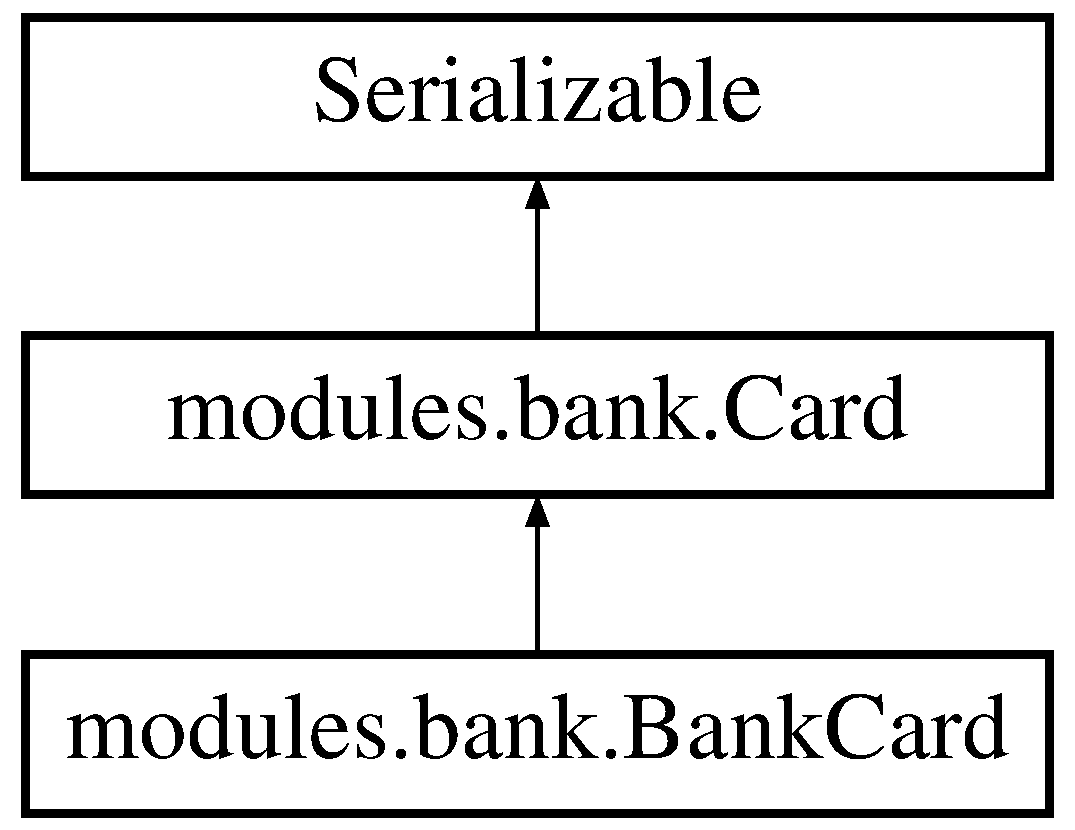
\includegraphics[height=3.000000cm]{classmodules_1_1bank_1_1_bank_card}
\end{center}
\end{figure}
\subsection*{Public Member Functions}
\begin{DoxyCompactItemize}
\item 
\mbox{\hyperlink{classmodules_1_1bank_1_1_bank_card_a1f5afbac8d1567ac220a7df1ad4c9741}{Bank\+Card}} (int n, String e)  throws Data\+Card\+Exception 
\item 
int \mbox{\hyperlink{classmodules_1_1bank_1_1_bank_card_ab72e9a1b96dc32bd70c373db4e4f6a17}{get\+Limit}} ()
\end{DoxyCompactItemize}
\subsection*{Additional Inherited Members}


\subsection{Detailed Description}
Class \mbox{\hyperlink{classmodules_1_1bank_1_1_bank_card}{Bank\+Card}} represents card that can be used in A\+TM \begin{DoxyAuthor}{Author}
Ernest Stachelski 
\end{DoxyAuthor}
\begin{DoxyVersion}{Version}
0.\+5 
\end{DoxyVersion}


\subsection{Constructor \& Destructor Documentation}
\mbox{\Hypertarget{classmodules_1_1bank_1_1_bank_card_a1f5afbac8d1567ac220a7df1ad4c9741}\label{classmodules_1_1bank_1_1_bank_card_a1f5afbac8d1567ac220a7df1ad4c9741}} 
\index{modules\+::bank\+::\+Bank\+Card@{modules\+::bank\+::\+Bank\+Card}!Bank\+Card@{Bank\+Card}}
\index{Bank\+Card@{Bank\+Card}!modules\+::bank\+::\+Bank\+Card@{modules\+::bank\+::\+Bank\+Card}}
\subsubsection{\texorpdfstring{Bank\+Card()}{BankCard()}}
{\footnotesize\ttfamily modules.\+bank.\+Bank\+Card.\+Bank\+Card (\begin{DoxyParamCaption}\item[{int}]{n,  }\item[{String}]{e }\end{DoxyParamCaption}) throws \mbox{\hyperlink{classsystem_1_1exceptions_1_1_data_card_exception}{Data\+Card\+Exception}}\hspace{0.3cm}{\ttfamily [inline]}}

Standard constructor 
\begin{DoxyParams}{Parameters}
{\em n} & represents \mbox{\hyperlink{classmodules_1_1bank_1_1_card}{Card}} number \\
\hline
{\em e} & represents \mbox{\hyperlink{classmodules_1_1bank_1_1_card}{Card}} expiration date \\
\hline
\end{DoxyParams}

\begin{DoxyExceptions}{Exceptions}
{\em Class\+Not\+Found\+Exception} & \\
\hline
{\em I\+O\+Exception} & \\
\hline
{\em Data\+Card\+Exception} & \\
\hline
\end{DoxyExceptions}


\subsection{Member Function Documentation}
\mbox{\Hypertarget{classmodules_1_1bank_1_1_bank_card_ab72e9a1b96dc32bd70c373db4e4f6a17}\label{classmodules_1_1bank_1_1_bank_card_ab72e9a1b96dc32bd70c373db4e4f6a17}} 
\index{modules\+::bank\+::\+Bank\+Card@{modules\+::bank\+::\+Bank\+Card}!get\+Limit@{get\+Limit}}
\index{get\+Limit@{get\+Limit}!modules\+::bank\+::\+Bank\+Card@{modules\+::bank\+::\+Bank\+Card}}
\subsubsection{\texorpdfstring{get\+Limit()}{getLimit()}}
{\footnotesize\ttfamily int modules.\+bank.\+Bank\+Card.\+get\+Limit (\begin{DoxyParamCaption}{ }\end{DoxyParamCaption})\hspace{0.3cm}{\ttfamily [inline]}}

Getter Limit in \mbox{\hyperlink{classmodules_1_1bank_1_1_bank_card}{Bank\+Card}} Limit in \mbox{\hyperlink{classmodules_1_1bank_1_1_bank}{Bank}} \mbox{\hyperlink{classmodules_1_1bank_1_1_card}{Card}} is 0 

The documentation for this class was generated from the following file\+:\begin{DoxyCompactItemize}
\item 
modules/bank/Bank\+Card.\+java\end{DoxyCompactItemize}

\hypertarget{classgui_1_1views_1_1_bank_view}{}\section{gui.\+views.\+Bank\+View Class Reference}
\label{classgui_1_1views_1_1_bank_view}\index{gui.\+views.\+Bank\+View@{gui.\+views.\+Bank\+View}}
Inheritance diagram for gui.\+views.\+Bank\+View\+:\begin{figure}[H]
\begin{center}
\leavevmode
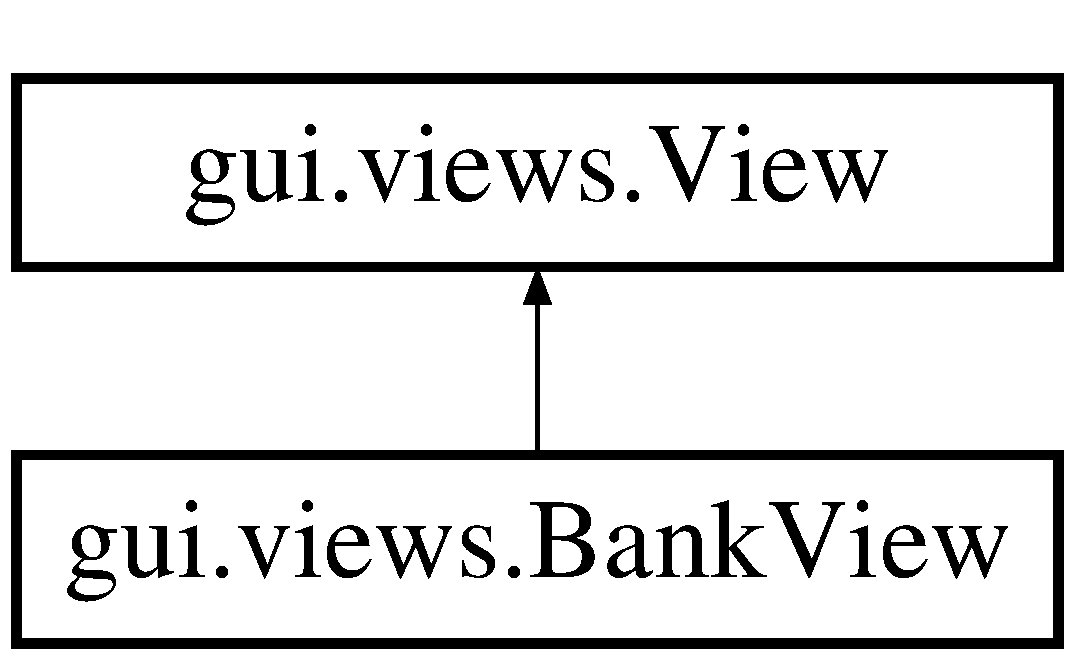
\includegraphics[height=2.000000cm]{classgui_1_1views_1_1_bank_view}
\end{center}
\end{figure}
\subsection*{Public Member Functions}
\begin{DoxyCompactItemize}
\item 
\mbox{\hyperlink{classgui_1_1views_1_1_bank_view_a89e587390ff1f18d69ef65b49fb8814d}{Bank\+View}} (Container display)
\item 
String \mbox{\hyperlink{classgui_1_1views_1_1_bank_view_ac5a8f5a66514f19790341a4ebfa8afa7}{get\+Name}} ()
\item 
void \mbox{\hyperlink{classgui_1_1views_1_1_bank_view_a60c0ec356e0a071e0a7c36b9aa9a7e55}{set\+Close\+Operation}} ()
\item 
void \mbox{\hyperlink{classgui_1_1views_1_1_bank_view_a01f6403f48d1ba9efd3bd9486170f68f}{update\+Lists}} ()
\item 
void \mbox{\hyperlink{classgui_1_1views_1_1_bank_view_a01f3aef7981cc38cbbde788cf508bb3e}{init\+Components}} ()
\item 
void \mbox{\hyperlink{classgui_1_1views_1_1_bank_view_a4e7ef9c3f0d99d799c09bc8a1c555ae0}{init\+Actions}} ()
\end{DoxyCompactItemize}
\subsection*{Additional Inherited Members}


\subsection{Constructor \& Destructor Documentation}
\mbox{\Hypertarget{classgui_1_1views_1_1_bank_view_a89e587390ff1f18d69ef65b49fb8814d}\label{classgui_1_1views_1_1_bank_view_a89e587390ff1f18d69ef65b49fb8814d}} 
\index{gui\+::views\+::\+Bank\+View@{gui\+::views\+::\+Bank\+View}!Bank\+View@{Bank\+View}}
\index{Bank\+View@{Bank\+View}!gui\+::views\+::\+Bank\+View@{gui\+::views\+::\+Bank\+View}}
\subsubsection{\texorpdfstring{Bank\+View()}{BankView()}}
{\footnotesize\ttfamily gui.\+views.\+Bank\+View.\+Bank\+View (\begin{DoxyParamCaption}\item[{Container}]{display }\end{DoxyParamCaption})\hspace{0.3cm}{\ttfamily [inline]}}

Construct runs at the start of program when views list is binded with names 
\begin{DoxyParams}{Parameters}
{\em display} & -\/ root pane where G\+UI will be render. \\
\hline
\end{DoxyParams}


\subsection{Member Function Documentation}
\mbox{\Hypertarget{classgui_1_1views_1_1_bank_view_ac5a8f5a66514f19790341a4ebfa8afa7}\label{classgui_1_1views_1_1_bank_view_ac5a8f5a66514f19790341a4ebfa8afa7}} 
\index{gui\+::views\+::\+Bank\+View@{gui\+::views\+::\+Bank\+View}!get\+Name@{get\+Name}}
\index{get\+Name@{get\+Name}!gui\+::views\+::\+Bank\+View@{gui\+::views\+::\+Bank\+View}}
\subsubsection{\texorpdfstring{get\+Name()}{getName()}}
{\footnotesize\ttfamily String gui.\+views.\+Bank\+View.\+get\+Name (\begin{DoxyParamCaption}{ }\end{DoxyParamCaption})\hspace{0.3cm}{\ttfamily [inline]}}

\begin{DoxySeeAlso}{See also}
\mbox{\hyperlink{classgui_1_1views_1_1_view}{View}} 
\end{DoxySeeAlso}
\mbox{\Hypertarget{classgui_1_1views_1_1_bank_view_a4e7ef9c3f0d99d799c09bc8a1c555ae0}\label{classgui_1_1views_1_1_bank_view_a4e7ef9c3f0d99d799c09bc8a1c555ae0}} 
\index{gui\+::views\+::\+Bank\+View@{gui\+::views\+::\+Bank\+View}!init\+Actions@{init\+Actions}}
\index{init\+Actions@{init\+Actions}!gui\+::views\+::\+Bank\+View@{gui\+::views\+::\+Bank\+View}}
\subsubsection{\texorpdfstring{init\+Actions()}{initActions()}}
{\footnotesize\ttfamily void gui.\+views.\+Bank\+View.\+init\+Actions (\begin{DoxyParamCaption}{ }\end{DoxyParamCaption})\hspace{0.3cm}{\ttfamily [inline]}}

Initialize action listeners for elements \mbox{\Hypertarget{classgui_1_1views_1_1_bank_view_a01f3aef7981cc38cbbde788cf508bb3e}\label{classgui_1_1views_1_1_bank_view_a01f3aef7981cc38cbbde788cf508bb3e}} 
\index{gui\+::views\+::\+Bank\+View@{gui\+::views\+::\+Bank\+View}!init\+Components@{init\+Components}}
\index{init\+Components@{init\+Components}!gui\+::views\+::\+Bank\+View@{gui\+::views\+::\+Bank\+View}}
\subsubsection{\texorpdfstring{init\+Components()}{initComponents()}}
{\footnotesize\ttfamily void gui.\+views.\+Bank\+View.\+init\+Components (\begin{DoxyParamCaption}{ }\end{DoxyParamCaption})\hspace{0.3cm}{\ttfamily [inline]}}

Initialize components -\/ sets look of objects and sets positions \mbox{\Hypertarget{classgui_1_1views_1_1_bank_view_a60c0ec356e0a071e0a7c36b9aa9a7e55}\label{classgui_1_1views_1_1_bank_view_a60c0ec356e0a071e0a7c36b9aa9a7e55}} 
\index{gui\+::views\+::\+Bank\+View@{gui\+::views\+::\+Bank\+View}!set\+Close\+Operation@{set\+Close\+Operation}}
\index{set\+Close\+Operation@{set\+Close\+Operation}!gui\+::views\+::\+Bank\+View@{gui\+::views\+::\+Bank\+View}}
\subsubsection{\texorpdfstring{set\+Close\+Operation()}{setCloseOperation()}}
{\footnotesize\ttfamily void gui.\+views.\+Bank\+View.\+set\+Close\+Operation (\begin{DoxyParamCaption}{ }\end{DoxyParamCaption})\hspace{0.3cm}{\ttfamily [inline]}}

Sets default close operation with action such as save before exit \mbox{\Hypertarget{classgui_1_1views_1_1_bank_view_a01f6403f48d1ba9efd3bd9486170f68f}\label{classgui_1_1views_1_1_bank_view_a01f6403f48d1ba9efd3bd9486170f68f}} 
\index{gui\+::views\+::\+Bank\+View@{gui\+::views\+::\+Bank\+View}!update\+Lists@{update\+Lists}}
\index{update\+Lists@{update\+Lists}!gui\+::views\+::\+Bank\+View@{gui\+::views\+::\+Bank\+View}}
\subsubsection{\texorpdfstring{update\+Lists()}{updateLists()}}
{\footnotesize\ttfamily void gui.\+views.\+Bank\+View.\+update\+Lists (\begin{DoxyParamCaption}{ }\end{DoxyParamCaption})\hspace{0.3cm}{\ttfamily [inline]}}

Updates client and cards lists before log in to specified bank 

The documentation for this class was generated from the following file\+:\begin{DoxyCompactItemize}
\item 
gui/views/Bank\+View.\+java\end{DoxyCompactItemize}

\hypertarget{classmodules_1_1bank_1_1_card}{}\section{modules.\+bank.\+Card Class Reference}
\label{classmodules_1_1bank_1_1_card}\index{modules.\+bank.\+Card@{modules.\+bank.\+Card}}
Inheritance diagram for modules.\+bank.\+Card\+:\begin{figure}[H]
\begin{center}
\leavevmode
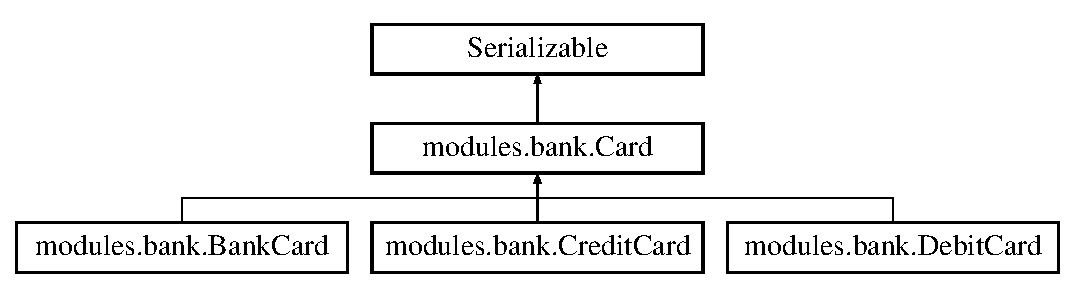
\includegraphics[height=3.000000cm]{classmodules_1_1bank_1_1_card}
\end{center}
\end{figure}
\subsection*{Public Member Functions}
\begin{DoxyCompactItemize}
\item 
\mbox{\Hypertarget{classmodules_1_1bank_1_1_card_a386f72c5b038bc8d80d10fd77b2c8db3}\label{classmodules_1_1bank_1_1_card_a386f72c5b038bc8d80d10fd77b2c8db3}} 
abstract int {\bfseries get\+Limit} ()
\item 
\mbox{\hyperlink{classmodules_1_1bank_1_1_card_a19e7ab54952594ea01d2f79bc984b4d1}{Card}} (int n, String e)  throws Data\+Card\+Exception
\item 
double \mbox{\hyperlink{classmodules_1_1bank_1_1_card_a62067906bc5ee5295a3e141cd4e9b9e8}{get\+Balance}} ()
\item 
void \mbox{\hyperlink{classmodules_1_1bank_1_1_card_a535c0ca771797c3d788fb1db64b16d15}{set\+Balance}} (double e)
\item 
int \mbox{\hyperlink{classmodules_1_1bank_1_1_card_a4d1b385624f4b1a3d2bea7a88082f4f3}{get\+Number}} ()
\item 
String \mbox{\hyperlink{classmodules_1_1bank_1_1_card_a4a06523d1698faecc6fb2f2c2345f810}{get\+Exp\+\_\+date}} ()
\item 
void \mbox{\hyperlink{classmodules_1_1bank_1_1_card_a2836bec99670bb580486005abfa86cac}{block\+Card}} ()
\item 
boolean \mbox{\hyperlink{classmodules_1_1bank_1_1_card_a2f5180fdbd0c6f73d1fb87af19a1f4be}{is\+Blocked}} ()
\item 
long \mbox{\hyperlink{classmodules_1_1bank_1_1_card_a91869b7c3dad648eb2470f27b0bb8a26}{get\+Id}} ()
\item 
void \mbox{\hyperlink{classmodules_1_1bank_1_1_card_a86370f2515d7612de7da603be14bad44}{set\+Number}} (int number)
\item 
String \mbox{\hyperlink{classmodules_1_1bank_1_1_card_aad416f3b110c7e08f3294b1b0cfd58d2}{to\+String}} ()
\item 
void \mbox{\hyperlink{classmodules_1_1bank_1_1_card_aa51b9d8df455d47e167192a911ca883b}{set\+Exp\+\_\+date}} (String exp\+\_\+date)
\end{DoxyCompactItemize}
\subsection*{Protected Attributes}
\begin{DoxyCompactItemize}
\item 
\mbox{\Hypertarget{classmodules_1_1bank_1_1_card_af4a87d2221c15317c9baf2c8003069d3}\label{classmodules_1_1bank_1_1_card_af4a87d2221c15317c9baf2c8003069d3}} 
int {\bfseries number}
\item 
\mbox{\Hypertarget{classmodules_1_1bank_1_1_card_ac8fef3d0557ee5cdf61aba050f0fd19d}\label{classmodules_1_1bank_1_1_card_ac8fef3d0557ee5cdf61aba050f0fd19d}} 
long {\bfseries id}
\item 
\mbox{\Hypertarget{classmodules_1_1bank_1_1_card_aed43b7a2f26e6473067b57a155987e23}\label{classmodules_1_1bank_1_1_card_aed43b7a2f26e6473067b57a155987e23}} 
double {\bfseries balance}
\item 
\mbox{\Hypertarget{classmodules_1_1bank_1_1_card_a61725dc4f6f2dce3b8d78eb8523645b8}\label{classmodules_1_1bank_1_1_card_a61725dc4f6f2dce3b8d78eb8523645b8}} 
String {\bfseries exp\+\_\+date}
\item 
\mbox{\Hypertarget{classmodules_1_1bank_1_1_card_aa5ff463df6e0a2b49513652b9435955b}\label{classmodules_1_1bank_1_1_card_aa5ff463df6e0a2b49513652b9435955b}} 
boolean {\bfseries blocked} = false
\end{DoxyCompactItemize}


\subsection{Detailed Description}
Abstract Class \mbox{\hyperlink{classmodules_1_1bank_1_1_card}{Card}} represents Account \mbox{\hyperlink{classmodules_1_1bank_1_1_card}{Card}} \begin{DoxyAuthor}{Author}
Ernest Stachelski 
\end{DoxyAuthor}
\begin{DoxyVersion}{Version}
0.\+5 
\end{DoxyVersion}


\subsection{Constructor \& Destructor Documentation}
\mbox{\Hypertarget{classmodules_1_1bank_1_1_card_a19e7ab54952594ea01d2f79bc984b4d1}\label{classmodules_1_1bank_1_1_card_a19e7ab54952594ea01d2f79bc984b4d1}} 
\index{modules\+::bank\+::\+Card@{modules\+::bank\+::\+Card}!Card@{Card}}
\index{Card@{Card}!modules\+::bank\+::\+Card@{modules\+::bank\+::\+Card}}
\subsubsection{\texorpdfstring{Card()}{Card()}}
{\footnotesize\ttfamily modules.\+bank.\+Card.\+Card (\begin{DoxyParamCaption}\item[{int}]{n,  }\item[{String}]{e }\end{DoxyParamCaption}) throws \mbox{\hyperlink{classsystem_1_1exceptions_1_1_data_card_exception}{Data\+Card\+Exception}}\hspace{0.3cm}{\ttfamily [inline]}}

Standard Constructor 
\begin{DoxyParams}{Parameters}
{\em n} & represents \mbox{\hyperlink{classmodules_1_1bank_1_1_card}{Card}} name \\
\hline
{\em e} & represents expiration date \\
\hline
\end{DoxyParams}

\begin{DoxyExceptions}{Exceptions}
{\em Class\+Not\+Found\+Exception} & \\
\hline
{\em I\+O\+Exception} & \\
\hline
{\em Data\+Card\+Exception} & \\
\hline
\end{DoxyExceptions}


\subsection{Member Function Documentation}
\mbox{\Hypertarget{classmodules_1_1bank_1_1_card_a2836bec99670bb580486005abfa86cac}\label{classmodules_1_1bank_1_1_card_a2836bec99670bb580486005abfa86cac}} 
\index{modules\+::bank\+::\+Card@{modules\+::bank\+::\+Card}!block\+Card@{block\+Card}}
\index{block\+Card@{block\+Card}!modules\+::bank\+::\+Card@{modules\+::bank\+::\+Card}}
\subsubsection{\texorpdfstring{block\+Card()}{blockCard()}}
{\footnotesize\ttfamily void modules.\+bank.\+Card.\+block\+Card (\begin{DoxyParamCaption}{ }\end{DoxyParamCaption})\hspace{0.3cm}{\ttfamily [inline]}}

Blocks \mbox{\hyperlink{classmodules_1_1bank_1_1_card}{Card}} \mbox{\Hypertarget{classmodules_1_1bank_1_1_card_a62067906bc5ee5295a3e141cd4e9b9e8}\label{classmodules_1_1bank_1_1_card_a62067906bc5ee5295a3e141cd4e9b9e8}} 
\index{modules\+::bank\+::\+Card@{modules\+::bank\+::\+Card}!get\+Balance@{get\+Balance}}
\index{get\+Balance@{get\+Balance}!modules\+::bank\+::\+Card@{modules\+::bank\+::\+Card}}
\subsubsection{\texorpdfstring{get\+Balance()}{getBalance()}}
{\footnotesize\ttfamily double modules.\+bank.\+Card.\+get\+Balance (\begin{DoxyParamCaption}{ }\end{DoxyParamCaption})\hspace{0.3cm}{\ttfamily [inline]}}

Getter Card/\+Account Balance \begin{DoxyReturn}{Returns}
double Balance 
\end{DoxyReturn}
\mbox{\Hypertarget{classmodules_1_1bank_1_1_card_a4a06523d1698faecc6fb2f2c2345f810}\label{classmodules_1_1bank_1_1_card_a4a06523d1698faecc6fb2f2c2345f810}} 
\index{modules\+::bank\+::\+Card@{modules\+::bank\+::\+Card}!get\+Exp\+\_\+date@{get\+Exp\+\_\+date}}
\index{get\+Exp\+\_\+date@{get\+Exp\+\_\+date}!modules\+::bank\+::\+Card@{modules\+::bank\+::\+Card}}
\subsubsection{\texorpdfstring{get\+Exp\+\_\+date()}{getExp\_date()}}
{\footnotesize\ttfamily String modules.\+bank.\+Card.\+get\+Exp\+\_\+date (\begin{DoxyParamCaption}{ }\end{DoxyParamCaption})\hspace{0.3cm}{\ttfamily [inline]}}

Getter Expiration Date \begin{DoxyReturn}{Returns}
String Expiration Date 
\end{DoxyReturn}
\mbox{\Hypertarget{classmodules_1_1bank_1_1_card_a91869b7c3dad648eb2470f27b0bb8a26}\label{classmodules_1_1bank_1_1_card_a91869b7c3dad648eb2470f27b0bb8a26}} 
\index{modules\+::bank\+::\+Card@{modules\+::bank\+::\+Card}!get\+Id@{get\+Id}}
\index{get\+Id@{get\+Id}!modules\+::bank\+::\+Card@{modules\+::bank\+::\+Card}}
\subsubsection{\texorpdfstring{get\+Id()}{getId()}}
{\footnotesize\ttfamily long modules.\+bank.\+Card.\+get\+Id (\begin{DoxyParamCaption}{ }\end{DoxyParamCaption})\hspace{0.3cm}{\ttfamily [inline]}}

Getter \mbox{\hyperlink{classmodules_1_1bank_1_1_card}{Card}} Id \begin{DoxyReturn}{Returns}
int Id 
\end{DoxyReturn}
\mbox{\Hypertarget{classmodules_1_1bank_1_1_card_a4d1b385624f4b1a3d2bea7a88082f4f3}\label{classmodules_1_1bank_1_1_card_a4d1b385624f4b1a3d2bea7a88082f4f3}} 
\index{modules\+::bank\+::\+Card@{modules\+::bank\+::\+Card}!get\+Number@{get\+Number}}
\index{get\+Number@{get\+Number}!modules\+::bank\+::\+Card@{modules\+::bank\+::\+Card}}
\subsubsection{\texorpdfstring{get\+Number()}{getNumber()}}
{\footnotesize\ttfamily int modules.\+bank.\+Card.\+get\+Number (\begin{DoxyParamCaption}{ }\end{DoxyParamCaption})\hspace{0.3cm}{\ttfamily [inline]}}

Getter \mbox{\hyperlink{classmodules_1_1bank_1_1_card}{Card}} Number \begin{DoxyReturn}{Returns}
int number 
\end{DoxyReturn}
\mbox{\Hypertarget{classmodules_1_1bank_1_1_card_a2f5180fdbd0c6f73d1fb87af19a1f4be}\label{classmodules_1_1bank_1_1_card_a2f5180fdbd0c6f73d1fb87af19a1f4be}} 
\index{modules\+::bank\+::\+Card@{modules\+::bank\+::\+Card}!is\+Blocked@{is\+Blocked}}
\index{is\+Blocked@{is\+Blocked}!modules\+::bank\+::\+Card@{modules\+::bank\+::\+Card}}
\subsubsection{\texorpdfstring{is\+Blocked()}{isBlocked()}}
{\footnotesize\ttfamily boolean modules.\+bank.\+Card.\+is\+Blocked (\begin{DoxyParamCaption}{ }\end{DoxyParamCaption})\hspace{0.3cm}{\ttfamily [inline]}}

Checks if card is blocked \begin{DoxyReturn}{Returns}
true if card is blocked 
\end{DoxyReturn}
\mbox{\Hypertarget{classmodules_1_1bank_1_1_card_a535c0ca771797c3d788fb1db64b16d15}\label{classmodules_1_1bank_1_1_card_a535c0ca771797c3d788fb1db64b16d15}} 
\index{modules\+::bank\+::\+Card@{modules\+::bank\+::\+Card}!set\+Balance@{set\+Balance}}
\index{set\+Balance@{set\+Balance}!modules\+::bank\+::\+Card@{modules\+::bank\+::\+Card}}
\subsubsection{\texorpdfstring{set\+Balance()}{setBalance()}}
{\footnotesize\ttfamily void modules.\+bank.\+Card.\+set\+Balance (\begin{DoxyParamCaption}\item[{double}]{e }\end{DoxyParamCaption})\hspace{0.3cm}{\ttfamily [inline]}}

Setter \mbox{\hyperlink{classmodules_1_1bank_1_1_card}{Card}} Balance 
\begin{DoxyParams}{Parameters}
{\em e} & represents money send to \mbox{\hyperlink{classmodules_1_1bank_1_1_card}{Card}} \\
\hline
\end{DoxyParams}
\mbox{\Hypertarget{classmodules_1_1bank_1_1_card_aa51b9d8df455d47e167192a911ca883b}\label{classmodules_1_1bank_1_1_card_aa51b9d8df455d47e167192a911ca883b}} 
\index{modules\+::bank\+::\+Card@{modules\+::bank\+::\+Card}!set\+Exp\+\_\+date@{set\+Exp\+\_\+date}}
\index{set\+Exp\+\_\+date@{set\+Exp\+\_\+date}!modules\+::bank\+::\+Card@{modules\+::bank\+::\+Card}}
\subsubsection{\texorpdfstring{set\+Exp\+\_\+date()}{setExp\_date()}}
{\footnotesize\ttfamily void modules.\+bank.\+Card.\+set\+Exp\+\_\+date (\begin{DoxyParamCaption}\item[{String}]{exp\+\_\+date }\end{DoxyParamCaption})\hspace{0.3cm}{\ttfamily [inline]}}

Getter for exp date 
\begin{DoxyParams}{Parameters}
{\em exp\+\_\+date} & \\
\hline
\end{DoxyParams}
\mbox{\Hypertarget{classmodules_1_1bank_1_1_card_a86370f2515d7612de7da603be14bad44}\label{classmodules_1_1bank_1_1_card_a86370f2515d7612de7da603be14bad44}} 
\index{modules\+::bank\+::\+Card@{modules\+::bank\+::\+Card}!set\+Number@{set\+Number}}
\index{set\+Number@{set\+Number}!modules\+::bank\+::\+Card@{modules\+::bank\+::\+Card}}
\subsubsection{\texorpdfstring{set\+Number()}{setNumber()}}
{\footnotesize\ttfamily void modules.\+bank.\+Card.\+set\+Number (\begin{DoxyParamCaption}\item[{int}]{number }\end{DoxyParamCaption})\hspace{0.3cm}{\ttfamily [inline]}}

Setter for card number 
\begin{DoxyParams}{Parameters}
{\em number} & \\
\hline
\end{DoxyParams}
\mbox{\Hypertarget{classmodules_1_1bank_1_1_card_aad416f3b110c7e08f3294b1b0cfd58d2}\label{classmodules_1_1bank_1_1_card_aad416f3b110c7e08f3294b1b0cfd58d2}} 
\index{modules\+::bank\+::\+Card@{modules\+::bank\+::\+Card}!to\+String@{to\+String}}
\index{to\+String@{to\+String}!modules\+::bank\+::\+Card@{modules\+::bank\+::\+Card}}
\subsubsection{\texorpdfstring{to\+String()}{toString()}}
{\footnotesize\ttfamily String modules.\+bank.\+Card.\+to\+String (\begin{DoxyParamCaption}{ }\end{DoxyParamCaption})\hspace{0.3cm}{\ttfamily [inline]}}

Converts object to string value 

The documentation for this class was generated from the following file\+:\begin{DoxyCompactItemize}
\item 
modules/bank/Card.\+java\end{DoxyCompactItemize}

\hypertarget{classmodules_1_1center_1_1_center}{}\section{modules.\+center.\+Center Class Reference}
\label{classmodules_1_1center_1_1_center}\index{modules.\+center.\+Center@{modules.\+center.\+Center}}
\subsection*{Public Member Functions}
\begin{DoxyCompactItemize}
\item 
\mbox{\hyperlink{classmodules_1_1center_1_1_center_aafc563c22cba49aff26c18c77c7e75d1}{Center}} ()  throws Class\+Not\+Found\+Exception, I\+O\+Exception 
\item 
Array\+List$<$ \mbox{\hyperlink{classmodules_1_1bank_1_1_bank}{Bank}} $>$ \mbox{\hyperlink{classmodules_1_1center_1_1_center_a61f9d6529ad2b0cadd05f2e3c5ae3980}{get\+Banks}} ()
\item 
Array\+List$<$ \mbox{\hyperlink{classmodules_1_1company_1_1_company}{Company}} $>$ \mbox{\hyperlink{classmodules_1_1center_1_1_center_a28a1f7e7802c5582806241aae1e22d01}{get\+Companies}} ()
\item 
Array\+List$<$ \mbox{\hyperlink{classmodules_1_1center_1_1_transaction}{Transaction}} $>$ \mbox{\hyperlink{classmodules_1_1center_1_1_center_ac7b4f20fffa160179ede31778f2773e0}{get\+Archive\+Transactions}} ()
\item 
Array\+List$<$ \mbox{\hyperlink{classmodules_1_1center_1_1_user}{User}} $>$ \mbox{\hyperlink{classmodules_1_1center_1_1_center_a5556fd8c6a1499a0f0ebf4e445be7853}{get\+Users}} ()
\item 
void \mbox{\hyperlink{classmodules_1_1center_1_1_center_aed29433137817c4fe2aae993e96a9d8e}{add\+User}} (String login, String password, String rights, String org\+Name)
\item 
void \mbox{\hyperlink{classmodules_1_1center_1_1_center_a01c47eb618c0c02f5e5df13431d6e8d6}{add\+Bank}} (String name)
\item 
void \mbox{\hyperlink{classmodules_1_1center_1_1_center_ae932db611d3a47791cc436ccc19e0311}{add\+Company}} (String name, String type)
\item 
void \mbox{\hyperlink{classmodules_1_1center_1_1_center_a0cc5fe3896c5cf301b89b0dc8b48afc2}{delete\+User}} (String login)
\item 
void \mbox{\hyperlink{classmodules_1_1center_1_1_center_a89031970f6b3cdc56028756583806062}{delete\+Bank}} (String name)
\item 
void \mbox{\hyperlink{classmodules_1_1center_1_1_center_ad4963e37162d6ce7ef17e00e36084853}{delete\+Company}} (String name)
\item 
void \mbox{\hyperlink{classmodules_1_1center_1_1_center_a542e2193495e6143fc6e950de4deee52}{edit\+Company}} (String name, String type, int order)
\item 
void \mbox{\hyperlink{classmodules_1_1center_1_1_center_a4b22f74fcfa6f3ca065f08f544749b46}{edit\+User}} (String login, String password, String role, String org\+Name, int order)
\item 
void \mbox{\hyperlink{classmodules_1_1center_1_1_center_a51e8ba3fb8ba9add102c99105443c331}{edit\+Bank}} (String name, int order)  throws Data\+Card\+Exception 
\item 
boolean \mbox{\hyperlink{classmodules_1_1center_1_1_center_aa7c6eab15974906f73962b7db4154a77}{handle\+Transaction}} (\mbox{\hyperlink{classmodules_1_1center_1_1_transaction}{Transaction}} trans)
\item 
Array\+List$<$ \mbox{\hyperlink{classmodules_1_1center_1_1_transaction}{Transaction}} $>$ \mbox{\hyperlink{classmodules_1_1center_1_1_center_ad841c33b5a86c38f7e4d3909928c2707}{get\+Archived\+Transaction}} (String query)
\item 
\mbox{\hyperlink{classmodules_1_1company_1_1_company}{Company}} \mbox{\hyperlink{classmodules_1_1center_1_1_center_a17d51c3fcb4d470a74a54e48f525cb51}{get\+Logged\+Company}} ()
\item 
void \mbox{\hyperlink{classmodules_1_1center_1_1_center_a752cd6c91d119e2e2c72ff844114548e}{set\+Logged\+Company}} (\mbox{\hyperlink{classmodules_1_1company_1_1_company}{Company}} logged\+Company)
\item 
\mbox{\hyperlink{classmodules_1_1bank_1_1_bank}{Bank}} \mbox{\hyperlink{classmodules_1_1center_1_1_center_ab52736c9e7079464e7488903193e96b3}{get\+Logged\+Bank}} ()
\item 
void \mbox{\hyperlink{classmodules_1_1center_1_1_center_ae78146080dffaba6b20b789d5558b775}{set\+Logged\+Bank}} (\mbox{\hyperlink{classmodules_1_1bank_1_1_bank}{Bank}} logged\+Bank)
\item 
void \mbox{\hyperlink{classmodules_1_1center_1_1_center_a32147ff3de943d0c2f658f5ea307c338}{set\+Banks}} (Array\+List$<$ \mbox{\hyperlink{classmodules_1_1bank_1_1_bank}{Bank}} $>$ banks)
\item 
Array\+List$<$ \mbox{\hyperlink{classmodules_1_1center_1_1_transaction}{Transaction}} $>$ \mbox{\hyperlink{classmodules_1_1center_1_1_center_ac5a4b03e0e634db0e9a019d19677594e}{get\+Archive\+\_\+transactions}} ()
\item 
void \mbox{\hyperlink{classmodules_1_1center_1_1_center_a751435feeb7bcd12bbe40fdead36b592}{set\+Archive\+\_\+transactions}} (Array\+List$<$ \mbox{\hyperlink{classmodules_1_1center_1_1_transaction}{Transaction}} $>$ archive\+\_\+transactions)
\end{DoxyCompactItemize}


\subsection{Detailed Description}
Class contains the list of all transactions ,center users and banks. \begin{DoxyAuthor}{Author}
Micha� Fi�o�czuk 
\end{DoxyAuthor}
\begin{DoxyVersion}{Version}
0.\+5 
\end{DoxyVersion}


\subsection{Constructor \& Destructor Documentation}
\mbox{\Hypertarget{classmodules_1_1center_1_1_center_aafc563c22cba49aff26c18c77c7e75d1}\label{classmodules_1_1center_1_1_center_aafc563c22cba49aff26c18c77c7e75d1}} 
\index{modules\+::center\+::\+Center@{modules\+::center\+::\+Center}!Center@{Center}}
\index{Center@{Center}!modules\+::center\+::\+Center@{modules\+::center\+::\+Center}}
\subsubsection{\texorpdfstring{Center()}{Center()}}
{\footnotesize\ttfamily modules.\+center.\+Center.\+Center (\begin{DoxyParamCaption}{ }\end{DoxyParamCaption}) throws Class\+Not\+Found\+Exception, I\+O\+Exception\hspace{0.3cm}{\ttfamily [inline]}}

Standard way to create \mbox{\hyperlink{classmodules_1_1center_1_1_center}{Center}} object 
\begin{DoxyExceptions}{Exceptions}
{\em Class\+Not\+Found\+Exception} & \\
\hline
{\em I\+O\+Exception} & \\
\hline
\end{DoxyExceptions}


\subsection{Member Function Documentation}
\mbox{\Hypertarget{classmodules_1_1center_1_1_center_a01c47eb618c0c02f5e5df13431d6e8d6}\label{classmodules_1_1center_1_1_center_a01c47eb618c0c02f5e5df13431d6e8d6}} 
\index{modules\+::center\+::\+Center@{modules\+::center\+::\+Center}!add\+Bank@{add\+Bank}}
\index{add\+Bank@{add\+Bank}!modules\+::center\+::\+Center@{modules\+::center\+::\+Center}}
\subsubsection{\texorpdfstring{add\+Bank()}{addBank()}}
{\footnotesize\ttfamily void modules.\+center.\+Center.\+add\+Bank (\begin{DoxyParamCaption}\item[{String}]{name }\end{DoxyParamCaption})\hspace{0.3cm}{\ttfamily [inline]}}

Adds new bank to the list 
\begin{DoxyParams}{Parameters}
{\em name} & -\/ String name of new bank \\
\hline
\end{DoxyParams}

\begin{DoxyExceptions}{Exceptions}
{\em Class\+Not\+Found\+Exception} & \\
\hline
{\em I\+O\+Exception} & \\
\hline
{\em Data\+Card\+Exception} & \\
\hline
\end{DoxyExceptions}
\mbox{\Hypertarget{classmodules_1_1center_1_1_center_ae932db611d3a47791cc436ccc19e0311}\label{classmodules_1_1center_1_1_center_ae932db611d3a47791cc436ccc19e0311}} 
\index{modules\+::center\+::\+Center@{modules\+::center\+::\+Center}!add\+Company@{add\+Company}}
\index{add\+Company@{add\+Company}!modules\+::center\+::\+Center@{modules\+::center\+::\+Center}}
\subsubsection{\texorpdfstring{add\+Company()}{addCompany()}}
{\footnotesize\ttfamily void modules.\+center.\+Center.\+add\+Company (\begin{DoxyParamCaption}\item[{String}]{name,  }\item[{String}]{type }\end{DoxyParamCaption})\hspace{0.3cm}{\ttfamily [inline]}}

Adds new company to the list 
\begin{DoxyParams}{Parameters}
{\em name} & -\/ String name of the company \\
\hline
{\em type} & -\/ String type of the company matches type in G\+UI \\
\hline
\end{DoxyParams}

\begin{DoxyExceptions}{Exceptions}
{\em Class\+Not\+Found\+Exception} & \\
\hline
{\em I\+O\+Exception} & \\
\hline
\end{DoxyExceptions}
\mbox{\Hypertarget{classmodules_1_1center_1_1_center_aed29433137817c4fe2aae993e96a9d8e}\label{classmodules_1_1center_1_1_center_aed29433137817c4fe2aae993e96a9d8e}} 
\index{modules\+::center\+::\+Center@{modules\+::center\+::\+Center}!add\+User@{add\+User}}
\index{add\+User@{add\+User}!modules\+::center\+::\+Center@{modules\+::center\+::\+Center}}
\subsubsection{\texorpdfstring{add\+User()}{addUser()}}
{\footnotesize\ttfamily void modules.\+center.\+Center.\+add\+User (\begin{DoxyParamCaption}\item[{String}]{login,  }\item[{String}]{password,  }\item[{String}]{rights,  }\item[{String}]{org\+Name }\end{DoxyParamCaption})\hspace{0.3cm}{\ttfamily [inline]}}

Adds new user to the list


\begin{DoxyParams}{Parameters}
{\em login} & -\/ String login of the user \\
\hline
{\em password} & -\/ String unencrypted password of the user \\
\hline
{\em rights} & -\/ String one option of\+: bank/company/admin \\
\hline
{\em org\+Name} & -\/ String Bank or Company name \\
\hline
\end{DoxyParams}
\mbox{\Hypertarget{classmodules_1_1center_1_1_center_a89031970f6b3cdc56028756583806062}\label{classmodules_1_1center_1_1_center_a89031970f6b3cdc56028756583806062}} 
\index{modules\+::center\+::\+Center@{modules\+::center\+::\+Center}!delete\+Bank@{delete\+Bank}}
\index{delete\+Bank@{delete\+Bank}!modules\+::center\+::\+Center@{modules\+::center\+::\+Center}}
\subsubsection{\texorpdfstring{delete\+Bank()}{deleteBank()}}
{\footnotesize\ttfamily void modules.\+center.\+Center.\+delete\+Bank (\begin{DoxyParamCaption}\item[{String}]{name }\end{DoxyParamCaption})\hspace{0.3cm}{\ttfamily [inline]}}

Deletes bank from the list 
\begin{DoxyParams}{Parameters}
{\em name} & -\/ String name of the bank to delete \\
\hline
\end{DoxyParams}
\mbox{\Hypertarget{classmodules_1_1center_1_1_center_ad4963e37162d6ce7ef17e00e36084853}\label{classmodules_1_1center_1_1_center_ad4963e37162d6ce7ef17e00e36084853}} 
\index{modules\+::center\+::\+Center@{modules\+::center\+::\+Center}!delete\+Company@{delete\+Company}}
\index{delete\+Company@{delete\+Company}!modules\+::center\+::\+Center@{modules\+::center\+::\+Center}}
\subsubsection{\texorpdfstring{delete\+Company()}{deleteCompany()}}
{\footnotesize\ttfamily void modules.\+center.\+Center.\+delete\+Company (\begin{DoxyParamCaption}\item[{String}]{name }\end{DoxyParamCaption})\hspace{0.3cm}{\ttfamily [inline]}}

Deletes company from the list 
\begin{DoxyParams}{Parameters}
{\em name} & -\/ String name of the company to delete \\
\hline
\end{DoxyParams}
\mbox{\Hypertarget{classmodules_1_1center_1_1_center_a0cc5fe3896c5cf301b89b0dc8b48afc2}\label{classmodules_1_1center_1_1_center_a0cc5fe3896c5cf301b89b0dc8b48afc2}} 
\index{modules\+::center\+::\+Center@{modules\+::center\+::\+Center}!delete\+User@{delete\+User}}
\index{delete\+User@{delete\+User}!modules\+::center\+::\+Center@{modules\+::center\+::\+Center}}
\subsubsection{\texorpdfstring{delete\+User()}{deleteUser()}}
{\footnotesize\ttfamily void modules.\+center.\+Center.\+delete\+User (\begin{DoxyParamCaption}\item[{String}]{login }\end{DoxyParamCaption})\hspace{0.3cm}{\ttfamily [inline]}}

Deletes user from the list 
\begin{DoxyParams}{Parameters}
{\em login} & -\/ String login of the user to delete \\
\hline
\end{DoxyParams}
\mbox{\Hypertarget{classmodules_1_1center_1_1_center_a51e8ba3fb8ba9add102c99105443c331}\label{classmodules_1_1center_1_1_center_a51e8ba3fb8ba9add102c99105443c331}} 
\index{modules\+::center\+::\+Center@{modules\+::center\+::\+Center}!edit\+Bank@{edit\+Bank}}
\index{edit\+Bank@{edit\+Bank}!modules\+::center\+::\+Center@{modules\+::center\+::\+Center}}
\subsubsection{\texorpdfstring{edit\+Bank()}{editBank()}}
{\footnotesize\ttfamily void modules.\+center.\+Center.\+edit\+Bank (\begin{DoxyParamCaption}\item[{String}]{name,  }\item[{int}]{order }\end{DoxyParamCaption}) throws \mbox{\hyperlink{classsystem_1_1exceptions_1_1_data_card_exception}{Data\+Card\+Exception}}\hspace{0.3cm}{\ttfamily [inline]}}

Updates one record from banks list 
\begin{DoxyParams}{Parameters}
{\em name} & -\/ String new name of the bank \\
\hline
{\em order} & -\/ Integer index of the bank in list \\
\hline
\end{DoxyParams}

\begin{DoxyExceptions}{Exceptions}
{\em Data\+Card\+Exception} & \\
\hline
\end{DoxyExceptions}
\mbox{\Hypertarget{classmodules_1_1center_1_1_center_a542e2193495e6143fc6e950de4deee52}\label{classmodules_1_1center_1_1_center_a542e2193495e6143fc6e950de4deee52}} 
\index{modules\+::center\+::\+Center@{modules\+::center\+::\+Center}!edit\+Company@{edit\+Company}}
\index{edit\+Company@{edit\+Company}!modules\+::center\+::\+Center@{modules\+::center\+::\+Center}}
\subsubsection{\texorpdfstring{edit\+Company()}{editCompany()}}
{\footnotesize\ttfamily void modules.\+center.\+Center.\+edit\+Company (\begin{DoxyParamCaption}\item[{String}]{name,  }\item[{String}]{type,  }\item[{int}]{order }\end{DoxyParamCaption})\hspace{0.3cm}{\ttfamily [inline]}}

Updates one record from companies list 
\begin{DoxyParams}{Parameters}
{\em name} & -\/ String new name of the company \\
\hline
{\em type} & -\/ String new type of the company (that matches one of the types from G\+UI) \\
\hline
{\em order} & -\/ Integer index of the record in list \\
\hline
\end{DoxyParams}
\mbox{\Hypertarget{classmodules_1_1center_1_1_center_a4b22f74fcfa6f3ca065f08f544749b46}\label{classmodules_1_1center_1_1_center_a4b22f74fcfa6f3ca065f08f544749b46}} 
\index{modules\+::center\+::\+Center@{modules\+::center\+::\+Center}!edit\+User@{edit\+User}}
\index{edit\+User@{edit\+User}!modules\+::center\+::\+Center@{modules\+::center\+::\+Center}}
\subsubsection{\texorpdfstring{edit\+User()}{editUser()}}
{\footnotesize\ttfamily void modules.\+center.\+Center.\+edit\+User (\begin{DoxyParamCaption}\item[{String}]{login,  }\item[{String}]{password,  }\item[{String}]{role,  }\item[{String}]{org\+Name,  }\item[{int}]{order }\end{DoxyParamCaption})\hspace{0.3cm}{\ttfamily [inline]}}

Updates one record from users list 
\begin{DoxyParams}{Parameters}
{\em login} & -\/ String new login of the user \\
\hline
{\em password} & -\/ String new unencrypted pass of the user \\
\hline
{\em role} & -\/ String new role of the user (that matches one of the role from G\+UI) \\
\hline
{\em order} & -\/ Integer index of the user in list \\
\hline
\end{DoxyParams}
\mbox{\Hypertarget{classmodules_1_1center_1_1_center_ac5a4b03e0e634db0e9a019d19677594e}\label{classmodules_1_1center_1_1_center_ac5a4b03e0e634db0e9a019d19677594e}} 
\index{modules\+::center\+::\+Center@{modules\+::center\+::\+Center}!get\+Archive\+\_\+transactions@{get\+Archive\+\_\+transactions}}
\index{get\+Archive\+\_\+transactions@{get\+Archive\+\_\+transactions}!modules\+::center\+::\+Center@{modules\+::center\+::\+Center}}
\subsubsection{\texorpdfstring{get\+Archive\+\_\+transactions()}{getArchive\_transactions()}}
{\footnotesize\ttfamily Array\+List$<$\mbox{\hyperlink{classmodules_1_1center_1_1_transaction}{Transaction}}$>$ modules.\+center.\+Center.\+get\+Archive\+\_\+transactions (\begin{DoxyParamCaption}{ }\end{DoxyParamCaption})\hspace{0.3cm}{\ttfamily [inline]}}

Gets full list of archived transactions \begin{DoxyReturn}{Returns}
Array\+List of transactions 
\end{DoxyReturn}
\mbox{\Hypertarget{classmodules_1_1center_1_1_center_ad841c33b5a86c38f7e4d3909928c2707}\label{classmodules_1_1center_1_1_center_ad841c33b5a86c38f7e4d3909928c2707}} 
\index{modules\+::center\+::\+Center@{modules\+::center\+::\+Center}!get\+Archived\+Transaction@{get\+Archived\+Transaction}}
\index{get\+Archived\+Transaction@{get\+Archived\+Transaction}!modules\+::center\+::\+Center@{modules\+::center\+::\+Center}}
\subsubsection{\texorpdfstring{get\+Archived\+Transaction()}{getArchivedTransaction()}}
{\footnotesize\ttfamily Array\+List$<$\mbox{\hyperlink{classmodules_1_1center_1_1_transaction}{Transaction}}$>$ modules.\+center.\+Center.\+get\+Archived\+Transaction (\begin{DoxyParamCaption}\item[{String}]{query }\end{DoxyParamCaption})\hspace{0.3cm}{\ttfamily [inline]}}

Returns the list of the transactions according to entered query


\begin{DoxyParams}{Parameters}
{\em query} & string -\/ properties of transaction you looking for, F\+O\+R\+M\+AT\+: Company\+:\+Bank\+:\+Card\+:amount\+:owner where\+: company is the name of company, bank is the name of the bank, card is card number, amount is amount\+:),date is date of the transaction(F\+O\+R\+M\+AT\+:D\+D-\/\+M\+M-\/\+R\+R\+RR) \\
\hline
\end{DoxyParams}
\begin{DoxyReturn}{Returns}
returns the requested transactions form the archives 
\end{DoxyReturn}
\mbox{\Hypertarget{classmodules_1_1center_1_1_center_ac7b4f20fffa160179ede31778f2773e0}\label{classmodules_1_1center_1_1_center_ac7b4f20fffa160179ede31778f2773e0}} 
\index{modules\+::center\+::\+Center@{modules\+::center\+::\+Center}!get\+Archive\+Transactions@{get\+Archive\+Transactions}}
\index{get\+Archive\+Transactions@{get\+Archive\+Transactions}!modules\+::center\+::\+Center@{modules\+::center\+::\+Center}}
\subsubsection{\texorpdfstring{get\+Archive\+Transactions()}{getArchiveTransactions()}}
{\footnotesize\ttfamily Array\+List$<$\mbox{\hyperlink{classmodules_1_1center_1_1_transaction}{Transaction}}$>$ modules.\+center.\+Center.\+get\+Archive\+Transactions (\begin{DoxyParamCaption}{ }\end{DoxyParamCaption})\hspace{0.3cm}{\ttfamily [inline]}}

Gets archived transactions list \begin{DoxyReturn}{Returns}
Array\+List complete transaction list 
\end{DoxyReturn}
\mbox{\Hypertarget{classmodules_1_1center_1_1_center_a61f9d6529ad2b0cadd05f2e3c5ae3980}\label{classmodules_1_1center_1_1_center_a61f9d6529ad2b0cadd05f2e3c5ae3980}} 
\index{modules\+::center\+::\+Center@{modules\+::center\+::\+Center}!get\+Banks@{get\+Banks}}
\index{get\+Banks@{get\+Banks}!modules\+::center\+::\+Center@{modules\+::center\+::\+Center}}
\subsubsection{\texorpdfstring{get\+Banks()}{getBanks()}}
{\footnotesize\ttfamily Array\+List$<$\mbox{\hyperlink{classmodules_1_1bank_1_1_bank}{Bank}}$>$ modules.\+center.\+Center.\+get\+Banks (\begin{DoxyParamCaption}{ }\end{DoxyParamCaption})\hspace{0.3cm}{\ttfamily [inline]}}

Gets banks list \begin{DoxyReturn}{Returns}
Array\+List complete banks list 
\end{DoxyReturn}
\mbox{\Hypertarget{classmodules_1_1center_1_1_center_a28a1f7e7802c5582806241aae1e22d01}\label{classmodules_1_1center_1_1_center_a28a1f7e7802c5582806241aae1e22d01}} 
\index{modules\+::center\+::\+Center@{modules\+::center\+::\+Center}!get\+Companies@{get\+Companies}}
\index{get\+Companies@{get\+Companies}!modules\+::center\+::\+Center@{modules\+::center\+::\+Center}}
\subsubsection{\texorpdfstring{get\+Companies()}{getCompanies()}}
{\footnotesize\ttfamily Array\+List$<$\mbox{\hyperlink{classmodules_1_1company_1_1_company}{Company}}$>$ modules.\+center.\+Center.\+get\+Companies (\begin{DoxyParamCaption}{ }\end{DoxyParamCaption})\hspace{0.3cm}{\ttfamily [inline]}}

Gets companies list \begin{DoxyReturn}{Returns}
Array\+List complete companies list 
\end{DoxyReturn}
\mbox{\Hypertarget{classmodules_1_1center_1_1_center_ab52736c9e7079464e7488903193e96b3}\label{classmodules_1_1center_1_1_center_ab52736c9e7079464e7488903193e96b3}} 
\index{modules\+::center\+::\+Center@{modules\+::center\+::\+Center}!get\+Logged\+Bank@{get\+Logged\+Bank}}
\index{get\+Logged\+Bank@{get\+Logged\+Bank}!modules\+::center\+::\+Center@{modules\+::center\+::\+Center}}
\subsubsection{\texorpdfstring{get\+Logged\+Bank()}{getLoggedBank()}}
{\footnotesize\ttfamily \mbox{\hyperlink{classmodules_1_1bank_1_1_bank}{Bank}} modules.\+center.\+Center.\+get\+Logged\+Bank (\begin{DoxyParamCaption}{ }\end{DoxyParamCaption})\hspace{0.3cm}{\ttfamily [inline]}}

Gets actual logged bank \begin{DoxyReturn}{Returns}
Bank 
\end{DoxyReturn}
\mbox{\Hypertarget{classmodules_1_1center_1_1_center_a17d51c3fcb4d470a74a54e48f525cb51}\label{classmodules_1_1center_1_1_center_a17d51c3fcb4d470a74a54e48f525cb51}} 
\index{modules\+::center\+::\+Center@{modules\+::center\+::\+Center}!get\+Logged\+Company@{get\+Logged\+Company}}
\index{get\+Logged\+Company@{get\+Logged\+Company}!modules\+::center\+::\+Center@{modules\+::center\+::\+Center}}
\subsubsection{\texorpdfstring{get\+Logged\+Company()}{getLoggedCompany()}}
{\footnotesize\ttfamily \mbox{\hyperlink{classmodules_1_1company_1_1_company}{Company}} modules.\+center.\+Center.\+get\+Logged\+Company (\begin{DoxyParamCaption}{ }\end{DoxyParamCaption})\hspace{0.3cm}{\ttfamily [inline]}}

Gets actual logged company \begin{DoxyReturn}{Returns}
Company 
\end{DoxyReturn}
\mbox{\Hypertarget{classmodules_1_1center_1_1_center_a5556fd8c6a1499a0f0ebf4e445be7853}\label{classmodules_1_1center_1_1_center_a5556fd8c6a1499a0f0ebf4e445be7853}} 
\index{modules\+::center\+::\+Center@{modules\+::center\+::\+Center}!get\+Users@{get\+Users}}
\index{get\+Users@{get\+Users}!modules\+::center\+::\+Center@{modules\+::center\+::\+Center}}
\subsubsection{\texorpdfstring{get\+Users()}{getUsers()}}
{\footnotesize\ttfamily Array\+List$<$\mbox{\hyperlink{classmodules_1_1center_1_1_user}{User}}$>$ modules.\+center.\+Center.\+get\+Users (\begin{DoxyParamCaption}{ }\end{DoxyParamCaption})\hspace{0.3cm}{\ttfamily [inline]}}

Gets users list \begin{DoxyReturn}{Returns}
Array\+List complete users list 
\end{DoxyReturn}
\mbox{\Hypertarget{classmodules_1_1center_1_1_center_aa7c6eab15974906f73962b7db4154a77}\label{classmodules_1_1center_1_1_center_aa7c6eab15974906f73962b7db4154a77}} 
\index{modules\+::center\+::\+Center@{modules\+::center\+::\+Center}!handle\+Transaction@{handle\+Transaction}}
\index{handle\+Transaction@{handle\+Transaction}!modules\+::center\+::\+Center@{modules\+::center\+::\+Center}}
\subsubsection{\texorpdfstring{handle\+Transaction()}{handleTransaction()}}
{\footnotesize\ttfamily boolean modules.\+center.\+Center.\+handle\+Transaction (\begin{DoxyParamCaption}\item[{\mbox{\hyperlink{classmodules_1_1center_1_1_transaction}{Transaction}}}]{trans }\end{DoxyParamCaption})\hspace{0.3cm}{\ttfamily [inline]}}

Passes transaction to the bank; \begin{DoxyAuthor}{Author}
Micha� Fi�o�czuk 
\end{DoxyAuthor}

\begin{DoxyParams}{Parameters}
{\em trans} & -\/ transaction object to check \\
\hline
\end{DoxyParams}
\begin{DoxyReturn}{Returns}
boolean true -\/ if transaction is accepted, false -\/ if transaction is rejected 
\end{DoxyReturn}
\mbox{\Hypertarget{classmodules_1_1center_1_1_center_a751435feeb7bcd12bbe40fdead36b592}\label{classmodules_1_1center_1_1_center_a751435feeb7bcd12bbe40fdead36b592}} 
\index{modules\+::center\+::\+Center@{modules\+::center\+::\+Center}!set\+Archive\+\_\+transactions@{set\+Archive\+\_\+transactions}}
\index{set\+Archive\+\_\+transactions@{set\+Archive\+\_\+transactions}!modules\+::center\+::\+Center@{modules\+::center\+::\+Center}}
\subsubsection{\texorpdfstring{set\+Archive\+\_\+transactions()}{setArchive\_transactions()}}
{\footnotesize\ttfamily void modules.\+center.\+Center.\+set\+Archive\+\_\+transactions (\begin{DoxyParamCaption}\item[{Array\+List$<$ \mbox{\hyperlink{classmodules_1_1center_1_1_transaction}{Transaction}} $>$}]{archive\+\_\+transactions }\end{DoxyParamCaption})\hspace{0.3cm}{\ttfamily [inline]}}

Sets list of archived transactions 
\begin{DoxyParams}{Parameters}
{\em archive\+\_\+transactions} & Array\+List of transactions \\
\hline
\end{DoxyParams}
\mbox{\Hypertarget{classmodules_1_1center_1_1_center_a32147ff3de943d0c2f658f5ea307c338}\label{classmodules_1_1center_1_1_center_a32147ff3de943d0c2f658f5ea307c338}} 
\index{modules\+::center\+::\+Center@{modules\+::center\+::\+Center}!set\+Banks@{set\+Banks}}
\index{set\+Banks@{set\+Banks}!modules\+::center\+::\+Center@{modules\+::center\+::\+Center}}
\subsubsection{\texorpdfstring{set\+Banks()}{setBanks()}}
{\footnotesize\ttfamily void modules.\+center.\+Center.\+set\+Banks (\begin{DoxyParamCaption}\item[{Array\+List$<$ \mbox{\hyperlink{classmodules_1_1bank_1_1_bank}{Bank}} $>$}]{banks }\end{DoxyParamCaption})\hspace{0.3cm}{\ttfamily [inline]}}

Sets list of banks for center 
\begin{DoxyParams}{Parameters}
{\em banks} & Array\+List of all banks \\
\hline
\end{DoxyParams}
\mbox{\Hypertarget{classmodules_1_1center_1_1_center_ae78146080dffaba6b20b789d5558b775}\label{classmodules_1_1center_1_1_center_ae78146080dffaba6b20b789d5558b775}} 
\index{modules\+::center\+::\+Center@{modules\+::center\+::\+Center}!set\+Logged\+Bank@{set\+Logged\+Bank}}
\index{set\+Logged\+Bank@{set\+Logged\+Bank}!modules\+::center\+::\+Center@{modules\+::center\+::\+Center}}
\subsubsection{\texorpdfstring{set\+Logged\+Bank()}{setLoggedBank()}}
{\footnotesize\ttfamily void modules.\+center.\+Center.\+set\+Logged\+Bank (\begin{DoxyParamCaption}\item[{\mbox{\hyperlink{classmodules_1_1bank_1_1_bank}{Bank}}}]{logged\+Bank }\end{DoxyParamCaption})\hspace{0.3cm}{\ttfamily [inline]}}

Sets actual logged bank 
\begin{DoxyParams}{Parameters}
{\em logged\+Bank} & Bank \\
\hline
\end{DoxyParams}
\mbox{\Hypertarget{classmodules_1_1center_1_1_center_a752cd6c91d119e2e2c72ff844114548e}\label{classmodules_1_1center_1_1_center_a752cd6c91d119e2e2c72ff844114548e}} 
\index{modules\+::center\+::\+Center@{modules\+::center\+::\+Center}!set\+Logged\+Company@{set\+Logged\+Company}}
\index{set\+Logged\+Company@{set\+Logged\+Company}!modules\+::center\+::\+Center@{modules\+::center\+::\+Center}}
\subsubsection{\texorpdfstring{set\+Logged\+Company()}{setLoggedCompany()}}
{\footnotesize\ttfamily void modules.\+center.\+Center.\+set\+Logged\+Company (\begin{DoxyParamCaption}\item[{\mbox{\hyperlink{classmodules_1_1company_1_1_company}{Company}}}]{logged\+Company }\end{DoxyParamCaption})\hspace{0.3cm}{\ttfamily [inline]}}

Sets actual logged company 
\begin{DoxyParams}{Parameters}
{\em logged\+Company} & Company \\
\hline
\end{DoxyParams}


The documentation for this class was generated from the following file\+:\begin{DoxyCompactItemize}
\item 
modules/center/Center.\+java\end{DoxyCompactItemize}

\hypertarget{classgui_1_1views_1_1_center_view}{}\section{gui.\+views.\+Center\+View Class Reference}
\label{classgui_1_1views_1_1_center_view}\index{gui.\+views.\+Center\+View@{gui.\+views.\+Center\+View}}
Inheritance diagram for gui.\+views.\+Center\+View\+:\begin{figure}[H]
\begin{center}
\leavevmode
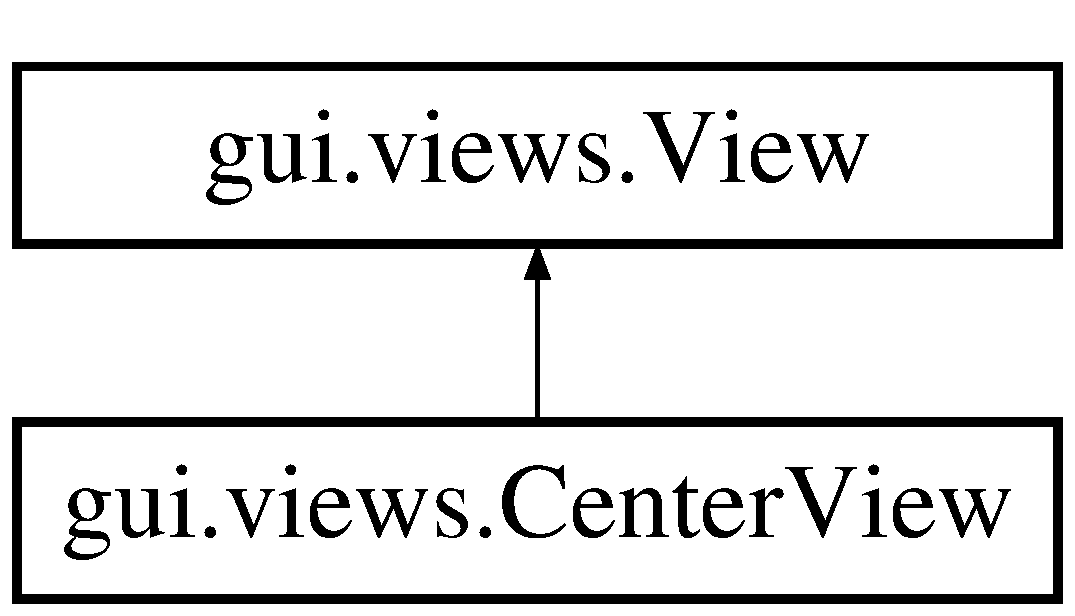
\includegraphics[height=2.000000cm]{classgui_1_1views_1_1_center_view}
\end{center}
\end{figure}
\subsection*{Public Member Functions}
\begin{DoxyCompactItemize}
\item 
\mbox{\hyperlink{classgui_1_1views_1_1_center_view_ab80e2efee3a410e5ccfc8ca285a81554}{Center\+View}} (Container display)
\item 
String \mbox{\hyperlink{classgui_1_1views_1_1_center_view_a9137970d5f143813a78b78d63316f9c3}{get\+Name}} ()
\item 
void \mbox{\hyperlink{classgui_1_1views_1_1_center_view_ae7ef58a077715b2730fca4ca104f420f}{set\+Close\+Operation}} ()
\item 
void \mbox{\hyperlink{classgui_1_1views_1_1_center_view_a88ac8cd9a5762534aa61168112bd8052}{init\+Components}} ()
\item 
void \mbox{\hyperlink{classgui_1_1views_1_1_center_view_acfa598e297fc3ef6a2649d4a188f5da4}{init\+Actions}} ()
\end{DoxyCompactItemize}
\subsection*{Additional Inherited Members}


\subsection{Constructor \& Destructor Documentation}
\mbox{\Hypertarget{classgui_1_1views_1_1_center_view_ab80e2efee3a410e5ccfc8ca285a81554}\label{classgui_1_1views_1_1_center_view_ab80e2efee3a410e5ccfc8ca285a81554}} 
\index{gui\+::views\+::\+Center\+View@{gui\+::views\+::\+Center\+View}!Center\+View@{Center\+View}}
\index{Center\+View@{Center\+View}!gui\+::views\+::\+Center\+View@{gui\+::views\+::\+Center\+View}}
\subsubsection{\texorpdfstring{Center\+View()}{CenterView()}}
{\footnotesize\ttfamily gui.\+views.\+Center\+View.\+Center\+View (\begin{DoxyParamCaption}\item[{Container}]{display }\end{DoxyParamCaption})\hspace{0.3cm}{\ttfamily [inline]}}

Basic constructor, set components


\begin{DoxyParams}{Parameters}
{\em display} & -\/ Container from actual frame \\
\hline
\end{DoxyParams}


\subsection{Member Function Documentation}
\mbox{\Hypertarget{classgui_1_1views_1_1_center_view_a9137970d5f143813a78b78d63316f9c3}\label{classgui_1_1views_1_1_center_view_a9137970d5f143813a78b78d63316f9c3}} 
\index{gui\+::views\+::\+Center\+View@{gui\+::views\+::\+Center\+View}!get\+Name@{get\+Name}}
\index{get\+Name@{get\+Name}!gui\+::views\+::\+Center\+View@{gui\+::views\+::\+Center\+View}}
\subsubsection{\texorpdfstring{get\+Name()}{getName()}}
{\footnotesize\ttfamily String gui.\+views.\+Center\+View.\+get\+Name (\begin{DoxyParamCaption}{ }\end{DoxyParamCaption})\hspace{0.3cm}{\ttfamily [inline]}}

\begin{DoxySeeAlso}{See also}
\mbox{\hyperlink{classgui_1_1views_1_1_view}{View}} 
\end{DoxySeeAlso}
\mbox{\Hypertarget{classgui_1_1views_1_1_center_view_acfa598e297fc3ef6a2649d4a188f5da4}\label{classgui_1_1views_1_1_center_view_acfa598e297fc3ef6a2649d4a188f5da4}} 
\index{gui\+::views\+::\+Center\+View@{gui\+::views\+::\+Center\+View}!init\+Actions@{init\+Actions}}
\index{init\+Actions@{init\+Actions}!gui\+::views\+::\+Center\+View@{gui\+::views\+::\+Center\+View}}
\subsubsection{\texorpdfstring{init\+Actions()}{initActions()}}
{\footnotesize\ttfamily void gui.\+views.\+Center\+View.\+init\+Actions (\begin{DoxyParamCaption}{ }\end{DoxyParamCaption})\hspace{0.3cm}{\ttfamily [inline]}}

Initialize action listeners for objects \mbox{\Hypertarget{classgui_1_1views_1_1_center_view_a88ac8cd9a5762534aa61168112bd8052}\label{classgui_1_1views_1_1_center_view_a88ac8cd9a5762534aa61168112bd8052}} 
\index{gui\+::views\+::\+Center\+View@{gui\+::views\+::\+Center\+View}!init\+Components@{init\+Components}}
\index{init\+Components@{init\+Components}!gui\+::views\+::\+Center\+View@{gui\+::views\+::\+Center\+View}}
\subsubsection{\texorpdfstring{init\+Components()}{initComponents()}}
{\footnotesize\ttfamily void gui.\+views.\+Center\+View.\+init\+Components (\begin{DoxyParamCaption}{ }\end{DoxyParamCaption})\hspace{0.3cm}{\ttfamily [inline]}}

Initialize components -\/ set look and feel of objects and set positions \mbox{\Hypertarget{classgui_1_1views_1_1_center_view_ae7ef58a077715b2730fca4ca104f420f}\label{classgui_1_1views_1_1_center_view_ae7ef58a077715b2730fca4ca104f420f}} 
\index{gui\+::views\+::\+Center\+View@{gui\+::views\+::\+Center\+View}!set\+Close\+Operation@{set\+Close\+Operation}}
\index{set\+Close\+Operation@{set\+Close\+Operation}!gui\+::views\+::\+Center\+View@{gui\+::views\+::\+Center\+View}}
\subsubsection{\texorpdfstring{set\+Close\+Operation()}{setCloseOperation()}}
{\footnotesize\ttfamily void gui.\+views.\+Center\+View.\+set\+Close\+Operation (\begin{DoxyParamCaption}{ }\end{DoxyParamCaption})\hspace{0.3cm}{\ttfamily [inline]}}

Sets default close operation with action such as save before exit 

The documentation for this class was generated from the following file\+:\begin{DoxyCompactItemize}
\item 
gui/views/Center\+View.\+java\end{DoxyCompactItemize}

\hypertarget{classmodules_1_1_client}{}\section{modules.\+Client Class Reference}
\label{classmodules_1_1_client}\index{modules.\+Client@{modules.\+Client}}
Inheritance diagram for modules.\+Client\+:\begin{figure}[H]
\begin{center}
\leavevmode
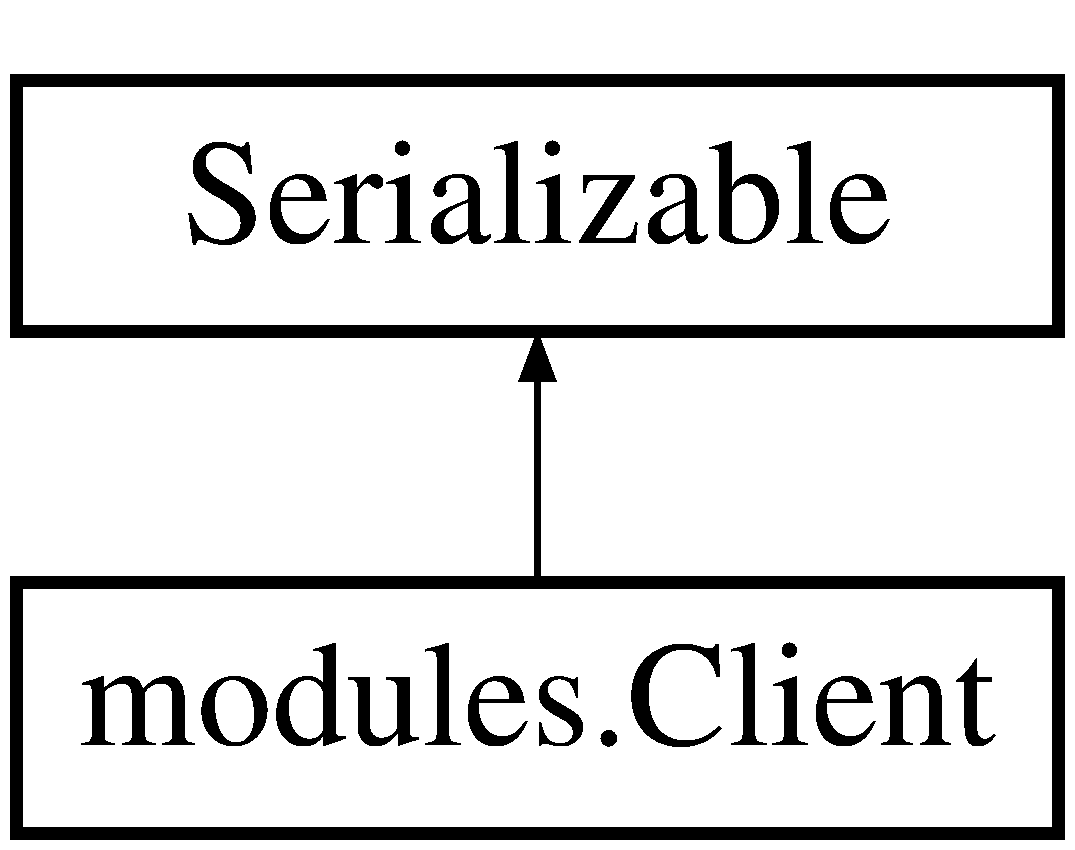
\includegraphics[height=2.000000cm]{classmodules_1_1_client}
\end{center}
\end{figure}
\subsection*{Public Member Functions}
\begin{DoxyCompactItemize}
\item 
\mbox{\hyperlink{classmodules_1_1_client_a50a7497cb32369672791ba33ace3264a}{Client}} (String n, String s, String p)
\item 
void \mbox{\hyperlink{classmodules_1_1_client_af9336218314937dc1a6820e84300b2bf}{add\+Card}} (\mbox{\hyperlink{classmodules_1_1bank_1_1_card}{Card}} c)
\item 
void \mbox{\hyperlink{classmodules_1_1_client_adc18605a931558c2483d48bf2cf36b0b}{delete\+Card}} (\mbox{\hyperlink{classmodules_1_1bank_1_1_card}{Card}} c)
\item 
void \mbox{\hyperlink{classmodules_1_1_client_a4fd4fe0ecb40203d81addd411abd18df}{delete\+Card}} (int number)  throws I\+O\+Exception, Class\+Not\+Found\+Exception 
\item 
String \mbox{\hyperlink{classmodules_1_1_client_abf135a1873bab2a59572e5208faa6b93}{get\+Pesel}} ()
\item 
String \mbox{\hyperlink{classmodules_1_1_client_afec5499055f7177339a5ff45bbcfff10}{get\+Name}} ()
\item 
String \mbox{\hyperlink{classmodules_1_1_client_a9edde75585aa9be7aebb9a9b818c6e12}{get\+Surname}} ()
\item 
String \mbox{\hyperlink{classmodules_1_1_client_a9ed6710e3598afe3dda7dac426c495fe}{to\+String}} ()
\item 
boolean \mbox{\hyperlink{classmodules_1_1_client_aa2b00842b4607600838347f2410c97ec}{has\+Card}} (\mbox{\hyperlink{classmodules_1_1bank_1_1_card}{Card}} card)
\item 
Array\+List$<$ \mbox{\hyperlink{classmodules_1_1bank_1_1_card}{Card}} $>$ \mbox{\hyperlink{classmodules_1_1_client_a4b56c055f3afc28546ea29b9579f79a1}{get\+Cards}} ()
\item 
boolean \mbox{\hyperlink{classmodules_1_1_client_a85eedfbdd0cdde608d7ce84aeb215e52}{has\+Card}} (int number)
\item 
void \mbox{\hyperlink{classmodules_1_1_client_acaea2a8b2086e298e3b22b86c409ecf4}{set\+Pesel}} (String pesel)
\item 
void \mbox{\hyperlink{classmodules_1_1_client_ae4fbf557127b160ce3de90af49bc3ff9}{set\+Name}} (String name)
\item 
void \mbox{\hyperlink{classmodules_1_1_client_a06f2d345b05093b2d61ca6cfc1f406a1}{set\+Surname}} (String surname)
\end{DoxyCompactItemize}


\subsection{Detailed Description}
Class represents specified bank customer \begin{DoxyAuthor}{Author}
Ernest Stachelski 
\end{DoxyAuthor}
\begin{DoxyVersion}{Version}
0.\+5 
\end{DoxyVersion}


\subsection{Constructor \& Destructor Documentation}
\mbox{\Hypertarget{classmodules_1_1_client_a50a7497cb32369672791ba33ace3264a}\label{classmodules_1_1_client_a50a7497cb32369672791ba33ace3264a}} 
\index{modules\+::\+Client@{modules\+::\+Client}!Client@{Client}}
\index{Client@{Client}!modules\+::\+Client@{modules\+::\+Client}}
\subsubsection{\texorpdfstring{Client()}{Client()}}
{\footnotesize\ttfamily modules.\+Client.\+Client (\begin{DoxyParamCaption}\item[{String}]{n,  }\item[{String}]{s,  }\item[{String}]{p }\end{DoxyParamCaption})\hspace{0.3cm}{\ttfamily [inline]}}

Standard constructor 
\begin{DoxyParams}{Parameters}
{\em n} & represents client name \\
\hline
{\em s} & represents client surname \\
\hline
{\em p} & represents client P\+E\+S\+EL \\
\hline
\end{DoxyParams}


\subsection{Member Function Documentation}
\mbox{\Hypertarget{classmodules_1_1_client_af9336218314937dc1a6820e84300b2bf}\label{classmodules_1_1_client_af9336218314937dc1a6820e84300b2bf}} 
\index{modules\+::\+Client@{modules\+::\+Client}!add\+Card@{add\+Card}}
\index{add\+Card@{add\+Card}!modules\+::\+Client@{modules\+::\+Client}}
\subsubsection{\texorpdfstring{add\+Card()}{addCard()}}
{\footnotesize\ttfamily void modules.\+Client.\+add\+Card (\begin{DoxyParamCaption}\item[{\mbox{\hyperlink{classmodules_1_1bank_1_1_card}{Card}}}]{c }\end{DoxyParamCaption})\hspace{0.3cm}{\ttfamily [inline]}}

Adds card for client 
\begin{DoxyParams}{Parameters}
{\em c} & -\/ card object that will be bind with \mbox{\hyperlink{classmodules_1_1_client}{Client}} \\
\hline
\end{DoxyParams}
\mbox{\Hypertarget{classmodules_1_1_client_adc18605a931558c2483d48bf2cf36b0b}\label{classmodules_1_1_client_adc18605a931558c2483d48bf2cf36b0b}} 
\index{modules\+::\+Client@{modules\+::\+Client}!delete\+Card@{delete\+Card}}
\index{delete\+Card@{delete\+Card}!modules\+::\+Client@{modules\+::\+Client}}
\subsubsection{\texorpdfstring{delete\+Card()}{deleteCard()}\hspace{0.1cm}{\footnotesize\ttfamily [1/2]}}
{\footnotesize\ttfamily void modules.\+Client.\+delete\+Card (\begin{DoxyParamCaption}\item[{\mbox{\hyperlink{classmodules_1_1bank_1_1_card}{Card}}}]{c }\end{DoxyParamCaption})\hspace{0.3cm}{\ttfamily [inline]}}

Removes client card 
\begin{DoxyParams}{Parameters}
{\em c} & -\/ card object that will be unbind from \mbox{\hyperlink{classmodules_1_1_client}{Client}} \\
\hline
\end{DoxyParams}
\mbox{\Hypertarget{classmodules_1_1_client_a4fd4fe0ecb40203d81addd411abd18df}\label{classmodules_1_1_client_a4fd4fe0ecb40203d81addd411abd18df}} 
\index{modules\+::\+Client@{modules\+::\+Client}!delete\+Card@{delete\+Card}}
\index{delete\+Card@{delete\+Card}!modules\+::\+Client@{modules\+::\+Client}}
\subsubsection{\texorpdfstring{delete\+Card()}{deleteCard()}\hspace{0.1cm}{\footnotesize\ttfamily [2/2]}}
{\footnotesize\ttfamily void modules.\+Client.\+delete\+Card (\begin{DoxyParamCaption}\item[{int}]{number }\end{DoxyParamCaption}) throws I\+O\+Exception, Class\+Not\+Found\+Exception\hspace{0.3cm}{\ttfamily [inline]}}

Removes client card 
\begin{DoxyParams}{Parameters}
{\em number} & -\/ index from the list of \mbox{\hyperlink{classmodules_1_1_client}{Client}}\textquotesingle{}s cards to delete \\
\hline
\end{DoxyParams}
\mbox{\Hypertarget{classmodules_1_1_client_a4b56c055f3afc28546ea29b9579f79a1}\label{classmodules_1_1_client_a4b56c055f3afc28546ea29b9579f79a1}} 
\index{modules\+::\+Client@{modules\+::\+Client}!get\+Cards@{get\+Cards}}
\index{get\+Cards@{get\+Cards}!modules\+::\+Client@{modules\+::\+Client}}
\subsubsection{\texorpdfstring{get\+Cards()}{getCards()}}
{\footnotesize\ttfamily Array\+List$<$\mbox{\hyperlink{classmodules_1_1bank_1_1_card}{Card}}$>$ modules.\+Client.\+get\+Cards (\begin{DoxyParamCaption}{ }\end{DoxyParamCaption})\hspace{0.3cm}{\ttfamily [inline]}}

Gets all cards list from client \begin{DoxyReturn}{Returns}

\end{DoxyReturn}
\mbox{\Hypertarget{classmodules_1_1_client_afec5499055f7177339a5ff45bbcfff10}\label{classmodules_1_1_client_afec5499055f7177339a5ff45bbcfff10}} 
\index{modules\+::\+Client@{modules\+::\+Client}!get\+Name@{get\+Name}}
\index{get\+Name@{get\+Name}!modules\+::\+Client@{modules\+::\+Client}}
\subsubsection{\texorpdfstring{get\+Name()}{getName()}}
{\footnotesize\ttfamily String modules.\+Client.\+get\+Name (\begin{DoxyParamCaption}{ }\end{DoxyParamCaption})\hspace{0.3cm}{\ttfamily [inline]}}

Getter Name \begin{DoxyReturn}{Returns}
string \mbox{\hyperlink{classmodules_1_1_client}{Client}} Name 
\end{DoxyReturn}
\mbox{\Hypertarget{classmodules_1_1_client_abf135a1873bab2a59572e5208faa6b93}\label{classmodules_1_1_client_abf135a1873bab2a59572e5208faa6b93}} 
\index{modules\+::\+Client@{modules\+::\+Client}!get\+Pesel@{get\+Pesel}}
\index{get\+Pesel@{get\+Pesel}!modules\+::\+Client@{modules\+::\+Client}}
\subsubsection{\texorpdfstring{get\+Pesel()}{getPesel()}}
{\footnotesize\ttfamily String modules.\+Client.\+get\+Pesel (\begin{DoxyParamCaption}{ }\end{DoxyParamCaption})\hspace{0.3cm}{\ttfamily [inline]}}

Getter P\+E\+S\+EL \begin{DoxyReturn}{Returns}
string P\+E\+S\+EL 
\end{DoxyReturn}
\mbox{\Hypertarget{classmodules_1_1_client_a9edde75585aa9be7aebb9a9b818c6e12}\label{classmodules_1_1_client_a9edde75585aa9be7aebb9a9b818c6e12}} 
\index{modules\+::\+Client@{modules\+::\+Client}!get\+Surname@{get\+Surname}}
\index{get\+Surname@{get\+Surname}!modules\+::\+Client@{modules\+::\+Client}}
\subsubsection{\texorpdfstring{get\+Surname()}{getSurname()}}
{\footnotesize\ttfamily String modules.\+Client.\+get\+Surname (\begin{DoxyParamCaption}{ }\end{DoxyParamCaption})\hspace{0.3cm}{\ttfamily [inline]}}

Getter Surname \begin{DoxyReturn}{Returns}
string \mbox{\hyperlink{classmodules_1_1_client}{Client}} Surname 
\end{DoxyReturn}
\mbox{\Hypertarget{classmodules_1_1_client_aa2b00842b4607600838347f2410c97ec}\label{classmodules_1_1_client_aa2b00842b4607600838347f2410c97ec}} 
\index{modules\+::\+Client@{modules\+::\+Client}!has\+Card@{has\+Card}}
\index{has\+Card@{has\+Card}!modules\+::\+Client@{modules\+::\+Client}}
\subsubsection{\texorpdfstring{has\+Card()}{hasCard()}\hspace{0.1cm}{\footnotesize\ttfamily [1/2]}}
{\footnotesize\ttfamily boolean modules.\+Client.\+has\+Card (\begin{DoxyParamCaption}\item[{\mbox{\hyperlink{classmodules_1_1bank_1_1_card}{Card}}}]{card }\end{DoxyParamCaption})\hspace{0.3cm}{\ttfamily [inline]}}

Checks if client own specified card 
\begin{DoxyParams}{Parameters}
{\em card} & -\/ card object to find \\
\hline
\end{DoxyParams}
\begin{DoxyReturn}{Returns}
owner flag 
\end{DoxyReturn}
\mbox{\Hypertarget{classmodules_1_1_client_a85eedfbdd0cdde608d7ce84aeb215e52}\label{classmodules_1_1_client_a85eedfbdd0cdde608d7ce84aeb215e52}} 
\index{modules\+::\+Client@{modules\+::\+Client}!has\+Card@{has\+Card}}
\index{has\+Card@{has\+Card}!modules\+::\+Client@{modules\+::\+Client}}
\subsubsection{\texorpdfstring{has\+Card()}{hasCard()}\hspace{0.1cm}{\footnotesize\ttfamily [2/2]}}
{\footnotesize\ttfamily boolean modules.\+Client.\+has\+Card (\begin{DoxyParamCaption}\item[{int}]{number }\end{DoxyParamCaption})\hspace{0.3cm}{\ttfamily [inline]}}

Checks if client own specified card 
\begin{DoxyParams}{Parameters}
{\em number} & -\/ card\textquotesingle{}s number to find \\
\hline
\end{DoxyParams}
\begin{DoxyReturn}{Returns}
owner flag 
\end{DoxyReturn}
\mbox{\Hypertarget{classmodules_1_1_client_ae4fbf557127b160ce3de90af49bc3ff9}\label{classmodules_1_1_client_ae4fbf557127b160ce3de90af49bc3ff9}} 
\index{modules\+::\+Client@{modules\+::\+Client}!set\+Name@{set\+Name}}
\index{set\+Name@{set\+Name}!modules\+::\+Client@{modules\+::\+Client}}
\subsubsection{\texorpdfstring{set\+Name()}{setName()}}
{\footnotesize\ttfamily void modules.\+Client.\+set\+Name (\begin{DoxyParamCaption}\item[{String}]{name }\end{DoxyParamCaption})\hspace{0.3cm}{\ttfamily [inline]}}

Sets new name 
\begin{DoxyParams}{Parameters}
{\em name} & -\/ string with new name \\
\hline
\end{DoxyParams}
\mbox{\Hypertarget{classmodules_1_1_client_acaea2a8b2086e298e3b22b86c409ecf4}\label{classmodules_1_1_client_acaea2a8b2086e298e3b22b86c409ecf4}} 
\index{modules\+::\+Client@{modules\+::\+Client}!set\+Pesel@{set\+Pesel}}
\index{set\+Pesel@{set\+Pesel}!modules\+::\+Client@{modules\+::\+Client}}
\subsubsection{\texorpdfstring{set\+Pesel()}{setPesel()}}
{\footnotesize\ttfamily void modules.\+Client.\+set\+Pesel (\begin{DoxyParamCaption}\item[{String}]{pesel }\end{DoxyParamCaption})\hspace{0.3cm}{\ttfamily [inline]}}

Sets new pesel value 
\begin{DoxyParams}{Parameters}
{\em pesel} & -\/ string with pesel \\
\hline
\end{DoxyParams}
\mbox{\Hypertarget{classmodules_1_1_client_a06f2d345b05093b2d61ca6cfc1f406a1}\label{classmodules_1_1_client_a06f2d345b05093b2d61ca6cfc1f406a1}} 
\index{modules\+::\+Client@{modules\+::\+Client}!set\+Surname@{set\+Surname}}
\index{set\+Surname@{set\+Surname}!modules\+::\+Client@{modules\+::\+Client}}
\subsubsection{\texorpdfstring{set\+Surname()}{setSurname()}}
{\footnotesize\ttfamily void modules.\+Client.\+set\+Surname (\begin{DoxyParamCaption}\item[{String}]{surname }\end{DoxyParamCaption})\hspace{0.3cm}{\ttfamily [inline]}}

Sets new surname 
\begin{DoxyParams}{Parameters}
{\em surname} & -\/ string with new surname \\
\hline
\end{DoxyParams}
\mbox{\Hypertarget{classmodules_1_1_client_a9ed6710e3598afe3dda7dac426c495fe}\label{classmodules_1_1_client_a9ed6710e3598afe3dda7dac426c495fe}} 
\index{modules\+::\+Client@{modules\+::\+Client}!to\+String@{to\+String}}
\index{to\+String@{to\+String}!modules\+::\+Client@{modules\+::\+Client}}
\subsubsection{\texorpdfstring{to\+String()}{toString()}}
{\footnotesize\ttfamily String modules.\+Client.\+to\+String (\begin{DoxyParamCaption}{ }\end{DoxyParamCaption})\hspace{0.3cm}{\ttfamily [inline]}}

Overridden method that converts object to string 

The documentation for this class was generated from the following file\+:\begin{DoxyCompactItemize}
\item 
modules/Client.\+java\end{DoxyCompactItemize}

\hypertarget{classmodules_1_1company_1_1_company}{}\section{modules.\+company.\+Company Class Reference}
\label{classmodules_1_1company_1_1_company}\index{modules.\+company.\+Company@{modules.\+company.\+Company}}
Inheritance diagram for modules.\+company.\+Company\+:\begin{figure}[H]
\begin{center}
\leavevmode
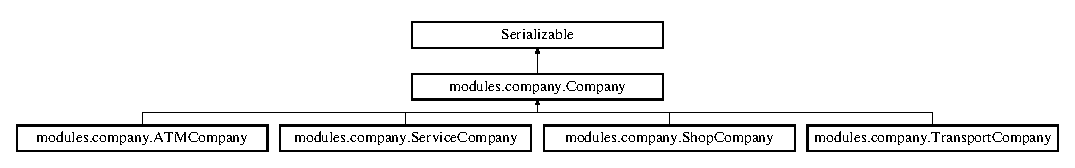
\includegraphics[height=1.810345cm]{classmodules_1_1company_1_1_company}
\end{center}
\end{figure}
\subsection*{Public Member Functions}
\begin{DoxyCompactItemize}
\item 
\mbox{\hyperlink{classmodules_1_1company_1_1_company_af325114b3fa48d956f62604aa443ce9c}{Company}} (String name)
\item 
String \mbox{\hyperlink{classmodules_1_1company_1_1_company_a26362cd08029dbca803df392d19e5b4d}{get\+Name}} ()
\item 
void \mbox{\hyperlink{classmodules_1_1company_1_1_company_a25b3de3a2188a6fc0d7245f16afeb11c}{set\+Name}} (String name)
\end{DoxyCompactItemize}
\subsection*{Protected Attributes}
\begin{DoxyCompactItemize}
\item 
\mbox{\Hypertarget{classmodules_1_1company_1_1_company_a851b0282951610951d2ac277ab24ac3b}\label{classmodules_1_1company_1_1_company_a851b0282951610951d2ac277ab24ac3b}} 
String {\bfseries name}
\end{DoxyCompactItemize}


\subsection{Detailed Description}
\mbox{\hyperlink{classmodules_1_1company_1_1_company}{Company}} is client of the Center. Represents the real firm which cooperate with center. \begin{DoxyAuthor}{Author}
Micha� Fi�o�czuk 
\end{DoxyAuthor}
\begin{DoxyVersion}{Version}
0.\+1 
\end{DoxyVersion}


\subsection{Constructor \& Destructor Documentation}
\mbox{\Hypertarget{classmodules_1_1company_1_1_company_af325114b3fa48d956f62604aa443ce9c}\label{classmodules_1_1company_1_1_company_af325114b3fa48d956f62604aa443ce9c}} 
\index{modules\+::company\+::\+Company@{modules\+::company\+::\+Company}!Company@{Company}}
\index{Company@{Company}!modules\+::company\+::\+Company@{modules\+::company\+::\+Company}}
\subsubsection{\texorpdfstring{Company()}{Company()}}
{\footnotesize\ttfamily modules.\+company.\+Company.\+Company (\begin{DoxyParamCaption}\item[{String}]{name }\end{DoxyParamCaption})\hspace{0.3cm}{\ttfamily [inline]}}

Standard way to create User object 
\begin{DoxyParams}{Parameters}
{\em id} & -\/ long ID number of the \mbox{\hyperlink{classmodules_1_1company_1_1_company}{Company}} \\
\hline
\end{DoxyParams}


\subsection{Member Function Documentation}
\mbox{\Hypertarget{classmodules_1_1company_1_1_company_a26362cd08029dbca803df392d19e5b4d}\label{classmodules_1_1company_1_1_company_a26362cd08029dbca803df392d19e5b4d}} 
\index{modules\+::company\+::\+Company@{modules\+::company\+::\+Company}!get\+Name@{get\+Name}}
\index{get\+Name@{get\+Name}!modules\+::company\+::\+Company@{modules\+::company\+::\+Company}}
\subsubsection{\texorpdfstring{get\+Name()}{getName()}}
{\footnotesize\ttfamily String modules.\+company.\+Company.\+get\+Name (\begin{DoxyParamCaption}{ }\end{DoxyParamCaption})\hspace{0.3cm}{\ttfamily [inline]}}

Getter of the name of the company \begin{DoxyReturn}{Returns}
name of the company 
\end{DoxyReturn}
\mbox{\Hypertarget{classmodules_1_1company_1_1_company_a25b3de3a2188a6fc0d7245f16afeb11c}\label{classmodules_1_1company_1_1_company_a25b3de3a2188a6fc0d7245f16afeb11c}} 
\index{modules\+::company\+::\+Company@{modules\+::company\+::\+Company}!set\+Name@{set\+Name}}
\index{set\+Name@{set\+Name}!modules\+::company\+::\+Company@{modules\+::company\+::\+Company}}
\subsubsection{\texorpdfstring{set\+Name()}{setName()}}
{\footnotesize\ttfamily void modules.\+company.\+Company.\+set\+Name (\begin{DoxyParamCaption}\item[{String}]{name }\end{DoxyParamCaption})\hspace{0.3cm}{\ttfamily [inline]}}

Setter of the name of the company 
\begin{DoxyParams}{Parameters}
{\em name} & new name of the company \\
\hline
\end{DoxyParams}


The documentation for this class was generated from the following file\+:\begin{DoxyCompactItemize}
\item 
modules/company/Company.\+java\end{DoxyCompactItemize}

\hypertarget{classgui_1_1views_1_1_company_view}{}\section{gui.\+views.\+Company\+View Class Reference}
\label{classgui_1_1views_1_1_company_view}\index{gui.\+views.\+Company\+View@{gui.\+views.\+Company\+View}}
Inheritance diagram for gui.\+views.\+Company\+View\+:\begin{figure}[H]
\begin{center}
\leavevmode
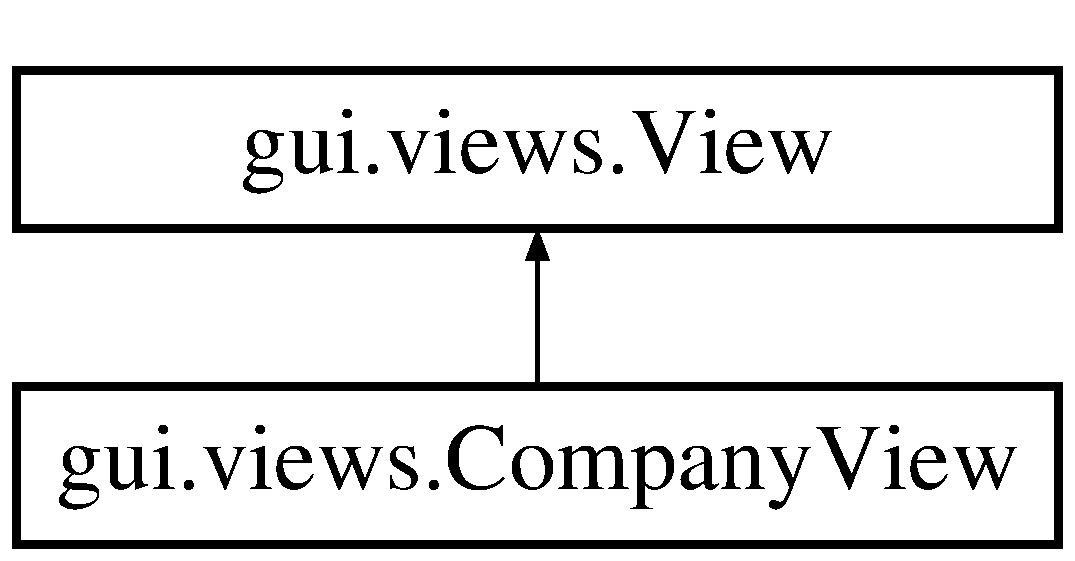
\includegraphics[height=2.000000cm]{classgui_1_1views_1_1_company_view}
\end{center}
\end{figure}
\subsection*{Public Member Functions}
\begin{DoxyCompactItemize}
\item 
\mbox{\hyperlink{classgui_1_1views_1_1_company_view_aa2a8ea9f17a43e5b24d54751833531b7}{Company\+View}} (Container display)
\item 
String \mbox{\hyperlink{classgui_1_1views_1_1_company_view_affe08c7aa7dfc02d86a18771aa2eb217}{get\+Name}} ()
\item 
void \mbox{\hyperlink{classgui_1_1views_1_1_company_view_abc80fd483dd89c441dbbe6a93ec7b213}{set\+Close\+Operation}} ()
\item 
void \mbox{\hyperlink{classgui_1_1views_1_1_company_view_a9a68d5e202ac887657159416dadb6887}{init\+Components}} ()
\item 
void \mbox{\hyperlink{classgui_1_1views_1_1_company_view_ab446dccf76b0195e7f09b9cd0e6d72a0}{init\+Actions}} ()
\end{DoxyCompactItemize}
\subsection*{Additional Inherited Members}


\subsection{Constructor \& Destructor Documentation}
\mbox{\Hypertarget{classgui_1_1views_1_1_company_view_aa2a8ea9f17a43e5b24d54751833531b7}\label{classgui_1_1views_1_1_company_view_aa2a8ea9f17a43e5b24d54751833531b7}} 
\index{gui\+::views\+::\+Company\+View@{gui\+::views\+::\+Company\+View}!Company\+View@{Company\+View}}
\index{Company\+View@{Company\+View}!gui\+::views\+::\+Company\+View@{gui\+::views\+::\+Company\+View}}
\subsubsection{\texorpdfstring{Company\+View()}{CompanyView()}}
{\footnotesize\ttfamily gui.\+views.\+Company\+View.\+Company\+View (\begin{DoxyParamCaption}\item[{Container}]{display }\end{DoxyParamCaption})\hspace{0.3cm}{\ttfamily [inline]}}

Basic constructor, set components


\begin{DoxyParams}{Parameters}
{\em display} & -\/ Container from actual frame \\
\hline
\end{DoxyParams}


\subsection{Member Function Documentation}
\mbox{\Hypertarget{classgui_1_1views_1_1_company_view_affe08c7aa7dfc02d86a18771aa2eb217}\label{classgui_1_1views_1_1_company_view_affe08c7aa7dfc02d86a18771aa2eb217}} 
\index{gui\+::views\+::\+Company\+View@{gui\+::views\+::\+Company\+View}!get\+Name@{get\+Name}}
\index{get\+Name@{get\+Name}!gui\+::views\+::\+Company\+View@{gui\+::views\+::\+Company\+View}}
\subsubsection{\texorpdfstring{get\+Name()}{getName()}}
{\footnotesize\ttfamily String gui.\+views.\+Company\+View.\+get\+Name (\begin{DoxyParamCaption}{ }\end{DoxyParamCaption})\hspace{0.3cm}{\ttfamily [inline]}}

\begin{DoxySeeAlso}{See also}
\mbox{\hyperlink{classgui_1_1views_1_1_view}{View}} 
\end{DoxySeeAlso}
\mbox{\Hypertarget{classgui_1_1views_1_1_company_view_ab446dccf76b0195e7f09b9cd0e6d72a0}\label{classgui_1_1views_1_1_company_view_ab446dccf76b0195e7f09b9cd0e6d72a0}} 
\index{gui\+::views\+::\+Company\+View@{gui\+::views\+::\+Company\+View}!init\+Actions@{init\+Actions}}
\index{init\+Actions@{init\+Actions}!gui\+::views\+::\+Company\+View@{gui\+::views\+::\+Company\+View}}
\subsubsection{\texorpdfstring{init\+Actions()}{initActions()}}
{\footnotesize\ttfamily void gui.\+views.\+Company\+View.\+init\+Actions (\begin{DoxyParamCaption}{ }\end{DoxyParamCaption})\hspace{0.3cm}{\ttfamily [inline]}}

Initialize action listeners for objects \mbox{\Hypertarget{classgui_1_1views_1_1_company_view_a9a68d5e202ac887657159416dadb6887}\label{classgui_1_1views_1_1_company_view_a9a68d5e202ac887657159416dadb6887}} 
\index{gui\+::views\+::\+Company\+View@{gui\+::views\+::\+Company\+View}!init\+Components@{init\+Components}}
\index{init\+Components@{init\+Components}!gui\+::views\+::\+Company\+View@{gui\+::views\+::\+Company\+View}}
\subsubsection{\texorpdfstring{init\+Components()}{initComponents()}}
{\footnotesize\ttfamily void gui.\+views.\+Company\+View.\+init\+Components (\begin{DoxyParamCaption}{ }\end{DoxyParamCaption})\hspace{0.3cm}{\ttfamily [inline]}}

Initialize components -\/ set look and feel of objects and set positions \mbox{\Hypertarget{classgui_1_1views_1_1_company_view_abc80fd483dd89c441dbbe6a93ec7b213}\label{classgui_1_1views_1_1_company_view_abc80fd483dd89c441dbbe6a93ec7b213}} 
\index{gui\+::views\+::\+Company\+View@{gui\+::views\+::\+Company\+View}!set\+Close\+Operation@{set\+Close\+Operation}}
\index{set\+Close\+Operation@{set\+Close\+Operation}!gui\+::views\+::\+Company\+View@{gui\+::views\+::\+Company\+View}}
\subsubsection{\texorpdfstring{set\+Close\+Operation()}{setCloseOperation()}}
{\footnotesize\ttfamily void gui.\+views.\+Company\+View.\+set\+Close\+Operation (\begin{DoxyParamCaption}{ }\end{DoxyParamCaption})\hspace{0.3cm}{\ttfamily [inline]}}

Sets default close operation with action such as save before exit 

The documentation for this class was generated from the following file\+:\begin{DoxyCompactItemize}
\item 
gui/views/Company\+View.\+java\end{DoxyCompactItemize}

\hypertarget{classmodules_1_1bank_1_1_credit_card}{}\section{modules.\+bank.\+Credit\+Card Class Reference}
\label{classmodules_1_1bank_1_1_credit_card}\index{modules.\+bank.\+Credit\+Card@{modules.\+bank.\+Credit\+Card}}
Inheritance diagram for modules.\+bank.\+Credit\+Card\+:\begin{figure}[H]
\begin{center}
\leavevmode
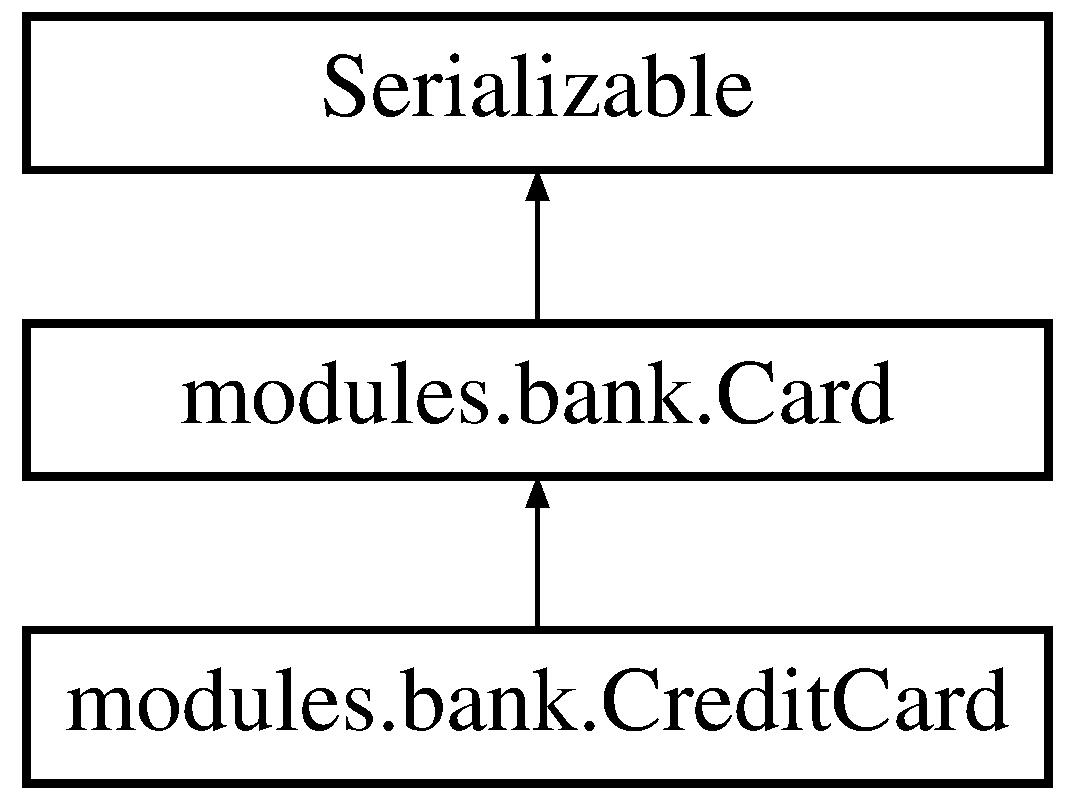
\includegraphics[height=3.000000cm]{classmodules_1_1bank_1_1_credit_card}
\end{center}
\end{figure}
\subsection*{Public Member Functions}
\begin{DoxyCompactItemize}
\item 
\mbox{\hyperlink{classmodules_1_1bank_1_1_credit_card_a8e6b9ecf2a7bfa17d3ac713caa427320}{Credit\+Card}} (int n, String e, int li)  throws Data\+Card\+Exception 
\item 
int \mbox{\hyperlink{classmodules_1_1bank_1_1_credit_card_a370decd7fd4895c200d38045ba60d939}{get\+Limit}} ()
\end{DoxyCompactItemize}
\subsection*{Additional Inherited Members}


\subsection{Detailed Description}
Class \mbox{\hyperlink{classmodules_1_1bank_1_1_credit_card}{Credit\+Card}} represents Credit\+Cards \begin{DoxyAuthor}{Author}
Ernest Stachelski 
\end{DoxyAuthor}
\begin{DoxyVersion}{Version}
0.\+5 
\end{DoxyVersion}


\subsection{Constructor \& Destructor Documentation}
\mbox{\Hypertarget{classmodules_1_1bank_1_1_credit_card_a8e6b9ecf2a7bfa17d3ac713caa427320}\label{classmodules_1_1bank_1_1_credit_card_a8e6b9ecf2a7bfa17d3ac713caa427320}} 
\index{modules\+::bank\+::\+Credit\+Card@{modules\+::bank\+::\+Credit\+Card}!Credit\+Card@{Credit\+Card}}
\index{Credit\+Card@{Credit\+Card}!modules\+::bank\+::\+Credit\+Card@{modules\+::bank\+::\+Credit\+Card}}
\subsubsection{\texorpdfstring{Credit\+Card()}{CreditCard()}}
{\footnotesize\ttfamily modules.\+bank.\+Credit\+Card.\+Credit\+Card (\begin{DoxyParamCaption}\item[{int}]{n,  }\item[{String}]{e,  }\item[{int}]{li }\end{DoxyParamCaption}) throws \mbox{\hyperlink{classsystem_1_1exceptions_1_1_data_card_exception}{Data\+Card\+Exception}}\hspace{0.3cm}{\ttfamily [inline]}}

\begin{DoxySeeAlso}{See also}
\mbox{\hyperlink{classmodules_1_1bank_1_1_card}{Card}} 
\end{DoxySeeAlso}


\subsection{Member Function Documentation}
\mbox{\Hypertarget{classmodules_1_1bank_1_1_credit_card_a370decd7fd4895c200d38045ba60d939}\label{classmodules_1_1bank_1_1_credit_card_a370decd7fd4895c200d38045ba60d939}} 
\index{modules\+::bank\+::\+Credit\+Card@{modules\+::bank\+::\+Credit\+Card}!get\+Limit@{get\+Limit}}
\index{get\+Limit@{get\+Limit}!modules\+::bank\+::\+Credit\+Card@{modules\+::bank\+::\+Credit\+Card}}
\subsubsection{\texorpdfstring{get\+Limit()}{getLimit()}}
{\footnotesize\ttfamily int modules.\+bank.\+Credit\+Card.\+get\+Limit (\begin{DoxyParamCaption}{ }\end{DoxyParamCaption})\hspace{0.3cm}{\ttfamily [inline]}}

Getter int Limit 

The documentation for this class was generated from the following file\+:\begin{DoxyCompactItemize}
\item 
modules/bank/Credit\+Card.\+java\end{DoxyCompactItemize}

\hypertarget{classsystem_1_1_database}{}\section{system.\+Database Class Reference}
\label{classsystem_1_1_database}\index{system.\+Database@{system.\+Database}}
\subsection*{Public Member Functions}
\begin{DoxyCompactItemize}
\item 
Array\+List$<$ \mbox{\hyperlink{classmodules_1_1center_1_1_user}{User}} $>$ \mbox{\hyperlink{classsystem_1_1_database_a563b32594ca62b2a365614df76f88a32}{R\+User}} ()  throws I\+O\+Exception, Class\+Not\+Found\+Exception 
\item 
Array\+List$<$ \mbox{\hyperlink{classmodules_1_1center_1_1_transaction}{Transaction}} $>$ \mbox{\hyperlink{classsystem_1_1_database_a699e545bc13bed8b01d1fa3748915656}{R\+Transaction}} ()  throws I\+O\+Exception, Class\+Not\+Found\+Exception
\item 
Array\+List$<$ \mbox{\hyperlink{classmodules_1_1company_1_1_company}{Company}} $>$ \mbox{\hyperlink{classsystem_1_1_database_a8aa0cd11f470af2f79e39447ded74416}{R\+Company}} ()  throws I\+O\+Exception, Class\+Not\+Found\+Exception
\item 
Array\+List$<$ \mbox{\hyperlink{classmodules_1_1bank_1_1_bank}{Bank}} $>$ \mbox{\hyperlink{classsystem_1_1_database_a1cd62e343cf922e01a0c78507793797d}{R\+Bank}} ()  throws I\+O\+Exception, Class\+Not\+Found\+Exception, Data\+Card\+Exception
\item 
Array\+List$<$ \mbox{\hyperlink{classmodules_1_1_client}{Client}} $>$ \mbox{\hyperlink{classsystem_1_1_database_a7fa9b0351cb06cb2791c1315363d58ed}{R\+Client}} ()  throws I\+O\+Exception, Class\+Not\+Found\+Exception
\item 
Array\+List$<$ \mbox{\hyperlink{classmodules_1_1bank_1_1_card}{Card}} $>$ \mbox{\hyperlink{classsystem_1_1_database_aa5a502f945de7e737fa11ffedf2a708e}{R\+Card}} ()  throws I\+O\+Exception, Class\+Not\+Found\+Exception, Data\+Card\+Exception
\item 
void \mbox{\hyperlink{classsystem_1_1_database_aaf148920dea060c0549a7482d2b5df33}{S\+User}} (Array\+List$<$ \mbox{\hyperlink{classmodules_1_1center_1_1_user}{User}} $>$ co)  throws I\+O\+Exception 
\item 
void \mbox{\hyperlink{classsystem_1_1_database_a4de6d2521c128d80081d8723cf13e155}{S\+Company}} (Array\+List$<$ \mbox{\hyperlink{classmodules_1_1company_1_1_company}{Company}} $>$ co)  throws I\+O\+Exception 
\item 
void \mbox{\hyperlink{classsystem_1_1_database_a64a050b14b8bb4b3dcecb34921291099}{S\+Client}} (Array\+List$<$ \mbox{\hyperlink{classmodules_1_1_client}{Client}} $>$ cl)  throws I\+O\+Exception 
\item 
void \mbox{\hyperlink{classsystem_1_1_database_ab4e8d37f1334b4a6f4ff60ab6c743ee3}{S\+Bank}} (Array\+List$<$ \mbox{\hyperlink{classmodules_1_1bank_1_1_bank}{Bank}} $>$ ba)  throws I\+O\+Exception
\item 
void \mbox{\hyperlink{classsystem_1_1_database_a94a0d7fe7179035d06ab24bf07968543}{S\+Card}} (Array\+List$<$ \mbox{\hyperlink{classmodules_1_1bank_1_1_card}{Card}} $>$ ca)  throws I\+O\+Exception 
\item 
void \mbox{\hyperlink{classsystem_1_1_database_a1a8335a4171ef7faf63e803fb844d7a0}{S\+Transaction}} (Array\+List$<$ \mbox{\hyperlink{classmodules_1_1center_1_1_transaction}{Transaction}} $>$ tr)  throws I\+O\+Exception 
\end{DoxyCompactItemize}


\subsection{Detailed Description}
\mbox{\hyperlink{classsystem_1_1_database}{Database}} works on project files \begin{DoxyAuthor}{Author}
Ernest Stachelski 
\end{DoxyAuthor}
\begin{DoxyVersion}{Version}
0.\+04 
\end{DoxyVersion}


\subsection{Member Function Documentation}
\mbox{\Hypertarget{classsystem_1_1_database_a1cd62e343cf922e01a0c78507793797d}\label{classsystem_1_1_database_a1cd62e343cf922e01a0c78507793797d}} 
\index{system\+::\+Database@{system\+::\+Database}!R\+Bank@{R\+Bank}}
\index{R\+Bank@{R\+Bank}!system\+::\+Database@{system\+::\+Database}}
\subsubsection{\texorpdfstring{R\+Bank()}{RBank()}}
{\footnotesize\ttfamily Array\+List$<$\mbox{\hyperlink{classmodules_1_1bank_1_1_bank}{Bank}}$>$ system.\+Database.\+R\+Bank (\begin{DoxyParamCaption}{ }\end{DoxyParamCaption}) throws I\+O\+Exception, Class\+Not\+Found\+Exception, \mbox{\hyperlink{classsystem_1_1exceptions_1_1_data_card_exception}{Data\+Card\+Exception}}\hspace{0.3cm}{\ttfamily [inline]}}

Reads Banks file \begin{DoxyReturn}{Returns}
Array\+List Banks 
\end{DoxyReturn}

\begin{DoxyExceptions}{Exceptions}
{\em I\+O\+Exception} & \\
\hline
{\em Class\+Not\+Found\+Exception} & \\
\hline
{\em Data\+Card\+Exception} & \\
\hline
\end{DoxyExceptions}
\mbox{\Hypertarget{classsystem_1_1_database_aa5a502f945de7e737fa11ffedf2a708e}\label{classsystem_1_1_database_aa5a502f945de7e737fa11ffedf2a708e}} 
\index{system\+::\+Database@{system\+::\+Database}!R\+Card@{R\+Card}}
\index{R\+Card@{R\+Card}!system\+::\+Database@{system\+::\+Database}}
\subsubsection{\texorpdfstring{R\+Card()}{RCard()}}
{\footnotesize\ttfamily Array\+List$<$\mbox{\hyperlink{classmodules_1_1bank_1_1_card}{Card}}$>$ system.\+Database.\+R\+Card (\begin{DoxyParamCaption}{ }\end{DoxyParamCaption}) throws I\+O\+Exception, Class\+Not\+Found\+Exception, \mbox{\hyperlink{classsystem_1_1exceptions_1_1_data_card_exception}{Data\+Card\+Exception}}\hspace{0.3cm}{\ttfamily [inline]}}

Reads Clients file \begin{DoxyReturn}{Returns}
Array\+List Clients 
\end{DoxyReturn}

\begin{DoxyExceptions}{Exceptions}
{\em I\+O\+Exception} & \\
\hline
{\em Class\+Not\+Found\+Exception} & \\
\hline
{\em Data\+Card\+Exception} & \\
\hline
\end{DoxyExceptions}
\mbox{\Hypertarget{classsystem_1_1_database_a7fa9b0351cb06cb2791c1315363d58ed}\label{classsystem_1_1_database_a7fa9b0351cb06cb2791c1315363d58ed}} 
\index{system\+::\+Database@{system\+::\+Database}!R\+Client@{R\+Client}}
\index{R\+Client@{R\+Client}!system\+::\+Database@{system\+::\+Database}}
\subsubsection{\texorpdfstring{R\+Client()}{RClient()}}
{\footnotesize\ttfamily Array\+List$<$\mbox{\hyperlink{classmodules_1_1_client}{Client}}$>$ system.\+Database.\+R\+Client (\begin{DoxyParamCaption}{ }\end{DoxyParamCaption}) throws I\+O\+Exception, Class\+Not\+Found\+Exception\hspace{0.3cm}{\ttfamily [inline]}}

Reads Clients file \begin{DoxyReturn}{Returns}
Array\+List Clients 
\end{DoxyReturn}

\begin{DoxyExceptions}{Exceptions}
{\em I\+O\+Exception} & \\
\hline
{\em Class\+Not\+Found\+Exception} & \\
\hline
\end{DoxyExceptions}
\mbox{\Hypertarget{classsystem_1_1_database_a8aa0cd11f470af2f79e39447ded74416}\label{classsystem_1_1_database_a8aa0cd11f470af2f79e39447ded74416}} 
\index{system\+::\+Database@{system\+::\+Database}!R\+Company@{R\+Company}}
\index{R\+Company@{R\+Company}!system\+::\+Database@{system\+::\+Database}}
\subsubsection{\texorpdfstring{R\+Company()}{RCompany()}}
{\footnotesize\ttfamily Array\+List$<$\mbox{\hyperlink{classmodules_1_1company_1_1_company}{Company}}$>$ system.\+Database.\+R\+Company (\begin{DoxyParamCaption}{ }\end{DoxyParamCaption}) throws I\+O\+Exception, Class\+Not\+Found\+Exception\hspace{0.3cm}{\ttfamily [inline]}}

Reads Companies file \begin{DoxyReturn}{Returns}
Array\+List Companies 
\end{DoxyReturn}

\begin{DoxyExceptions}{Exceptions}
{\em I\+O\+Exception} & \\
\hline
{\em Class\+Not\+Found\+Exception} & \\
\hline
\end{DoxyExceptions}
\mbox{\Hypertarget{classsystem_1_1_database_a699e545bc13bed8b01d1fa3748915656}\label{classsystem_1_1_database_a699e545bc13bed8b01d1fa3748915656}} 
\index{system\+::\+Database@{system\+::\+Database}!R\+Transaction@{R\+Transaction}}
\index{R\+Transaction@{R\+Transaction}!system\+::\+Database@{system\+::\+Database}}
\subsubsection{\texorpdfstring{R\+Transaction()}{RTransaction()}}
{\footnotesize\ttfamily Array\+List$<$\mbox{\hyperlink{classmodules_1_1center_1_1_transaction}{Transaction}}$>$ system.\+Database.\+R\+Transaction (\begin{DoxyParamCaption}{ }\end{DoxyParamCaption}) throws I\+O\+Exception, Class\+Not\+Found\+Exception\hspace{0.3cm}{\ttfamily [inline]}}

Reads Transactions file \begin{DoxyReturn}{Returns}
Array\+List Transactions 
\end{DoxyReturn}

\begin{DoxyExceptions}{Exceptions}
{\em I\+O\+Exception} & \\
\hline
{\em Class\+Not\+Found\+Exception} & \\
\hline
\end{DoxyExceptions}
\mbox{\Hypertarget{classsystem_1_1_database_a563b32594ca62b2a365614df76f88a32}\label{classsystem_1_1_database_a563b32594ca62b2a365614df76f88a32}} 
\index{system\+::\+Database@{system\+::\+Database}!R\+User@{R\+User}}
\index{R\+User@{R\+User}!system\+::\+Database@{system\+::\+Database}}
\subsubsection{\texorpdfstring{R\+User()}{RUser()}}
{\footnotesize\ttfamily Array\+List$<$\mbox{\hyperlink{classmodules_1_1center_1_1_user}{User}}$>$ system.\+Database.\+R\+User (\begin{DoxyParamCaption}{ }\end{DoxyParamCaption}) throws I\+O\+Exception, Class\+Not\+Found\+Exception\hspace{0.3cm}{\ttfamily [inline]}}

Reads Users file \begin{DoxyReturn}{Returns}
Array\+List Users 
\end{DoxyReturn}

\begin{DoxyExceptions}{Exceptions}
{\em I\+O\+Exception} & \\
\hline
{\em Class\+Not\+Found\+Exception} & \\
\hline
\end{DoxyExceptions}
\mbox{\Hypertarget{classsystem_1_1_database_ab4e8d37f1334b4a6f4ff60ab6c743ee3}\label{classsystem_1_1_database_ab4e8d37f1334b4a6f4ff60ab6c743ee3}} 
\index{system\+::\+Database@{system\+::\+Database}!S\+Bank@{S\+Bank}}
\index{S\+Bank@{S\+Bank}!system\+::\+Database@{system\+::\+Database}}
\subsubsection{\texorpdfstring{S\+Bank()}{SBank()}}
{\footnotesize\ttfamily void system.\+Database.\+S\+Bank (\begin{DoxyParamCaption}\item[{Array\+List$<$ \mbox{\hyperlink{classmodules_1_1bank_1_1_bank}{Bank}} $>$}]{ba }\end{DoxyParamCaption}) throws I\+O\+Exception\hspace{0.3cm}{\ttfamily [inline]}}

Saves Banks List 
\begin{DoxyParams}{Parameters}
{\em ba} & represents list of all banks \\
\hline
\end{DoxyParams}

\begin{DoxyExceptions}{Exceptions}
{\em I\+O\+Exception} & \\
\hline
\end{DoxyExceptions}
\mbox{\Hypertarget{classsystem_1_1_database_a94a0d7fe7179035d06ab24bf07968543}\label{classsystem_1_1_database_a94a0d7fe7179035d06ab24bf07968543}} 
\index{system\+::\+Database@{system\+::\+Database}!S\+Card@{S\+Card}}
\index{S\+Card@{S\+Card}!system\+::\+Database@{system\+::\+Database}}
\subsubsection{\texorpdfstring{S\+Card()}{SCard()}}
{\footnotesize\ttfamily void system.\+Database.\+S\+Card (\begin{DoxyParamCaption}\item[{Array\+List$<$ \mbox{\hyperlink{classmodules_1_1bank_1_1_card}{Card}} $>$}]{ca }\end{DoxyParamCaption}) throws I\+O\+Exception\hspace{0.3cm}{\ttfamily [inline]}}

Saves Cards List 
\begin{DoxyParams}{Parameters}
{\em ca} & represents list of all cards \\
\hline
\end{DoxyParams}

\begin{DoxyExceptions}{Exceptions}
{\em I\+O\+Exception} & \\
\hline
\end{DoxyExceptions}
\mbox{\Hypertarget{classsystem_1_1_database_a64a050b14b8bb4b3dcecb34921291099}\label{classsystem_1_1_database_a64a050b14b8bb4b3dcecb34921291099}} 
\index{system\+::\+Database@{system\+::\+Database}!S\+Client@{S\+Client}}
\index{S\+Client@{S\+Client}!system\+::\+Database@{system\+::\+Database}}
\subsubsection{\texorpdfstring{S\+Client()}{SClient()}}
{\footnotesize\ttfamily void system.\+Database.\+S\+Client (\begin{DoxyParamCaption}\item[{Array\+List$<$ \mbox{\hyperlink{classmodules_1_1_client}{Client}} $>$}]{cl }\end{DoxyParamCaption}) throws I\+O\+Exception\hspace{0.3cm}{\ttfamily [inline]}}

Saves Cleints List 
\begin{DoxyParams}{Parameters}
{\em cl} & represents list of all clients \\
\hline
\end{DoxyParams}

\begin{DoxyExceptions}{Exceptions}
{\em I\+O\+Exception} & \\
\hline
\end{DoxyExceptions}
\mbox{\Hypertarget{classsystem_1_1_database_a4de6d2521c128d80081d8723cf13e155}\label{classsystem_1_1_database_a4de6d2521c128d80081d8723cf13e155}} 
\index{system\+::\+Database@{system\+::\+Database}!S\+Company@{S\+Company}}
\index{S\+Company@{S\+Company}!system\+::\+Database@{system\+::\+Database}}
\subsubsection{\texorpdfstring{S\+Company()}{SCompany()}}
{\footnotesize\ttfamily void system.\+Database.\+S\+Company (\begin{DoxyParamCaption}\item[{Array\+List$<$ \mbox{\hyperlink{classmodules_1_1company_1_1_company}{Company}} $>$}]{co }\end{DoxyParamCaption}) throws I\+O\+Exception\hspace{0.3cm}{\ttfamily [inline]}}

Saves Companies List 
\begin{DoxyParams}{Parameters}
{\em co} & represents list of all companies \\
\hline
\end{DoxyParams}

\begin{DoxyExceptions}{Exceptions}
{\em I\+O\+Exception} & \\
\hline
\end{DoxyExceptions}
\mbox{\Hypertarget{classsystem_1_1_database_a1a8335a4171ef7faf63e803fb844d7a0}\label{classsystem_1_1_database_a1a8335a4171ef7faf63e803fb844d7a0}} 
\index{system\+::\+Database@{system\+::\+Database}!S\+Transaction@{S\+Transaction}}
\index{S\+Transaction@{S\+Transaction}!system\+::\+Database@{system\+::\+Database}}
\subsubsection{\texorpdfstring{S\+Transaction()}{STransaction()}}
{\footnotesize\ttfamily void system.\+Database.\+S\+Transaction (\begin{DoxyParamCaption}\item[{Array\+List$<$ \mbox{\hyperlink{classmodules_1_1center_1_1_transaction}{Transaction}} $>$}]{tr }\end{DoxyParamCaption}) throws I\+O\+Exception\hspace{0.3cm}{\ttfamily [inline]}}

Saves Transactions List 
\begin{DoxyParams}{Parameters}
{\em tr} & represents list of all transactions \\
\hline
\end{DoxyParams}

\begin{DoxyExceptions}{Exceptions}
{\em I\+O\+Exception} & \\
\hline
\end{DoxyExceptions}
\mbox{\Hypertarget{classsystem_1_1_database_aaf148920dea060c0549a7482d2b5df33}\label{classsystem_1_1_database_aaf148920dea060c0549a7482d2b5df33}} 
\index{system\+::\+Database@{system\+::\+Database}!S\+User@{S\+User}}
\index{S\+User@{S\+User}!system\+::\+Database@{system\+::\+Database}}
\subsubsection{\texorpdfstring{S\+User()}{SUser()}}
{\footnotesize\ttfamily void system.\+Database.\+S\+User (\begin{DoxyParamCaption}\item[{Array\+List$<$ \mbox{\hyperlink{classmodules_1_1center_1_1_user}{User}} $>$}]{co }\end{DoxyParamCaption}) throws I\+O\+Exception\hspace{0.3cm}{\ttfamily [inline]}}

Saves User List 
\begin{DoxyParams}{Parameters}
{\em u} & represents list of all users \\
\hline
\end{DoxyParams}

\begin{DoxyExceptions}{Exceptions}
{\em I\+O\+Exception} & \\
\hline
\end{DoxyExceptions}


The documentation for this class was generated from the following file\+:\begin{DoxyCompactItemize}
\item 
system/Database.\+java\end{DoxyCompactItemize}

\hypertarget{classsystem_1_1exceptions_1_1_data_card_exception}{}\section{system.\+exceptions.\+Data\+Card\+Exception Class Reference}
\label{classsystem_1_1exceptions_1_1_data_card_exception}\index{system.\+exceptions.\+Data\+Card\+Exception@{system.\+exceptions.\+Data\+Card\+Exception}}
Inheritance diagram for system.\+exceptions.\+Data\+Card\+Exception\+:\begin{figure}[H]
\begin{center}
\leavevmode
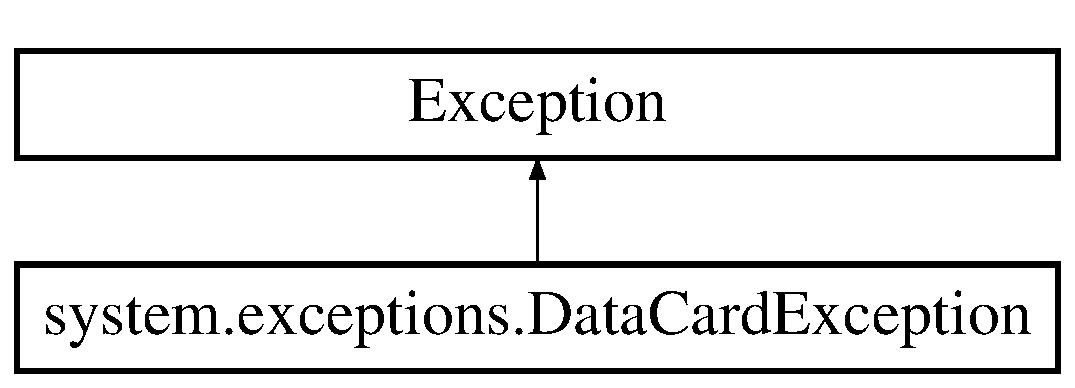
\includegraphics[height=2.000000cm]{classsystem_1_1exceptions_1_1_data_card_exception}
\end{center}
\end{figure}


\subsection{Detailed Description}
Checks months and length of Data in Card \begin{DoxyAuthor}{Author}
Ernest Stachelski 
\end{DoxyAuthor}
\begin{DoxyVersion}{Version}
0.\+1 
\end{DoxyVersion}


The documentation for this class was generated from the following file\+:\begin{DoxyCompactItemize}
\item 
system/exceptions/Data\+Card\+Exception.\+java\end{DoxyCompactItemize}

\hypertarget{classmodules_1_1bank_1_1_debit_card}{}\section{modules.\+bank.\+Debit\+Card Class Reference}
\label{classmodules_1_1bank_1_1_debit_card}\index{modules.\+bank.\+Debit\+Card@{modules.\+bank.\+Debit\+Card}}
Inheritance diagram for modules.\+bank.\+Debit\+Card\+:\begin{figure}[H]
\begin{center}
\leavevmode
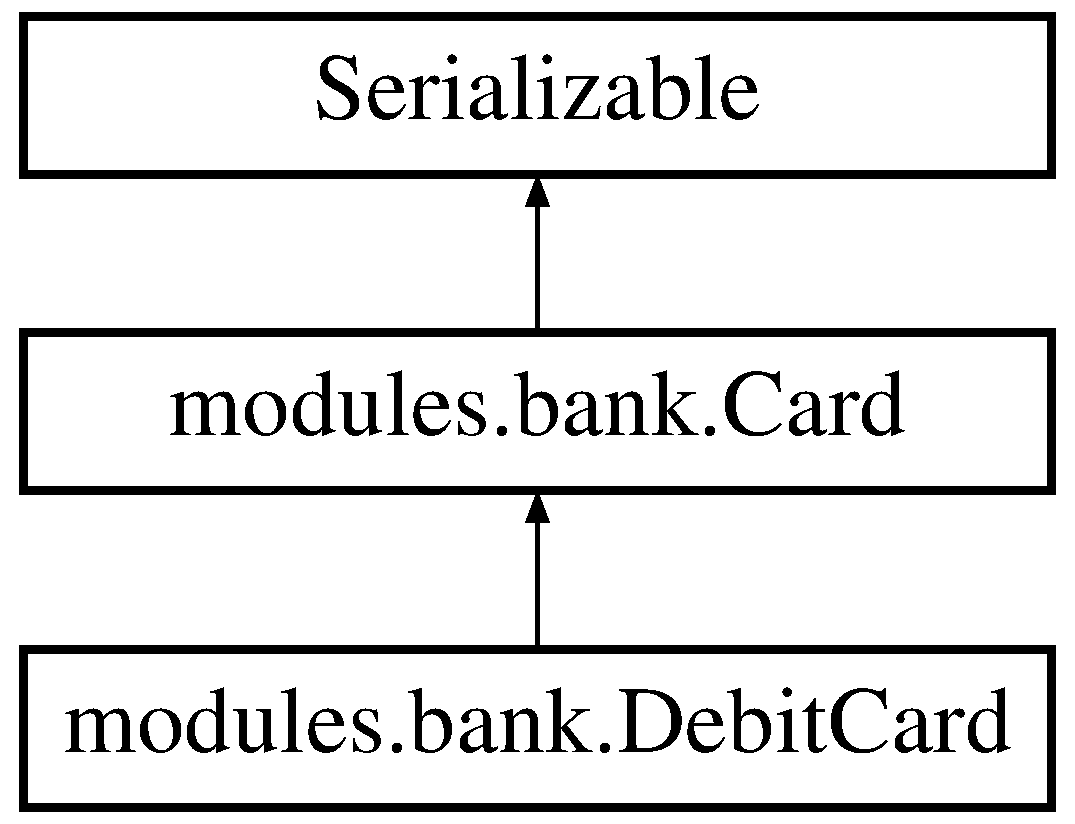
\includegraphics[height=3.000000cm]{classmodules_1_1bank_1_1_debit_card}
\end{center}
\end{figure}
\subsection*{Public Member Functions}
\begin{DoxyCompactItemize}
\item 
\mbox{\hyperlink{classmodules_1_1bank_1_1_debit_card_a8c1e64fb14ac49e486aa8e052cb29e80}{Debit\+Card}} (int n, String e)  throws Data\+Card\+Exception 
\item 
int \mbox{\hyperlink{classmodules_1_1bank_1_1_debit_card_acf3df8280f72ad26844cb04fdb9bb3ae}{get\+Limit}} ()
\end{DoxyCompactItemize}
\subsection*{Additional Inherited Members}


\subsection{Detailed Description}
Class \mbox{\hyperlink{classmodules_1_1bank_1_1_debit_card}{Debit\+Card}} represents card with creditworthiness \begin{DoxyAuthor}{Author}
Ernest Stachelski 
\end{DoxyAuthor}
\begin{DoxyVersion}{Version}
0.\+5 
\end{DoxyVersion}


\subsection{Constructor \& Destructor Documentation}
\mbox{\Hypertarget{classmodules_1_1bank_1_1_debit_card_a8c1e64fb14ac49e486aa8e052cb29e80}\label{classmodules_1_1bank_1_1_debit_card_a8c1e64fb14ac49e486aa8e052cb29e80}} 
\index{modules\+::bank\+::\+Debit\+Card@{modules\+::bank\+::\+Debit\+Card}!Debit\+Card@{Debit\+Card}}
\index{Debit\+Card@{Debit\+Card}!modules\+::bank\+::\+Debit\+Card@{modules\+::bank\+::\+Debit\+Card}}
\subsubsection{\texorpdfstring{Debit\+Card()}{DebitCard()}}
{\footnotesize\ttfamily modules.\+bank.\+Debit\+Card.\+Debit\+Card (\begin{DoxyParamCaption}\item[{int}]{n,  }\item[{String}]{e }\end{DoxyParamCaption}) throws \mbox{\hyperlink{classsystem_1_1exceptions_1_1_data_card_exception}{Data\+Card\+Exception}}\hspace{0.3cm}{\ttfamily [inline]}}

Standard constructor 
\begin{DoxyParams}{Parameters}
{\em n} & represents \mbox{\hyperlink{classmodules_1_1bank_1_1_card}{Card}} number \\
\hline
{\em e} & represents \mbox{\hyperlink{classmodules_1_1bank_1_1_card}{Card}} expiration date \\
\hline
\end{DoxyParams}

\begin{DoxyExceptions}{Exceptions}
{\em Class\+Not\+Found\+Exception} & \\
\hline
{\em I\+O\+Exception} & \\
\hline
{\em Data\+Card\+Exception} & \\
\hline
\end{DoxyExceptions}


\subsection{Member Function Documentation}
\mbox{\Hypertarget{classmodules_1_1bank_1_1_debit_card_acf3df8280f72ad26844cb04fdb9bb3ae}\label{classmodules_1_1bank_1_1_debit_card_acf3df8280f72ad26844cb04fdb9bb3ae}} 
\index{modules\+::bank\+::\+Debit\+Card@{modules\+::bank\+::\+Debit\+Card}!get\+Limit@{get\+Limit}}
\index{get\+Limit@{get\+Limit}!modules\+::bank\+::\+Debit\+Card@{modules\+::bank\+::\+Debit\+Card}}
\subsubsection{\texorpdfstring{get\+Limit()}{getLimit()}}
{\footnotesize\ttfamily int modules.\+bank.\+Debit\+Card.\+get\+Limit (\begin{DoxyParamCaption}{ }\end{DoxyParamCaption})\hspace{0.3cm}{\ttfamily [inline]}}

Getter Limit in \mbox{\hyperlink{classmodules_1_1bank_1_1_bank_card}{Bank\+Card}} Limit in credit card is 0 

The documentation for this class was generated from the following file\+:\begin{DoxyCompactItemize}
\item 
modules/bank/Debit\+Card.\+java\end{DoxyCompactItemize}

\hypertarget{classgui_1_1views_1_1_login_view}{}\section{gui.\+views.\+Login\+View Class Reference}
\label{classgui_1_1views_1_1_login_view}\index{gui.\+views.\+Login\+View@{gui.\+views.\+Login\+View}}
Inheritance diagram for gui.\+views.\+Login\+View\+:\begin{figure}[H]
\begin{center}
\leavevmode
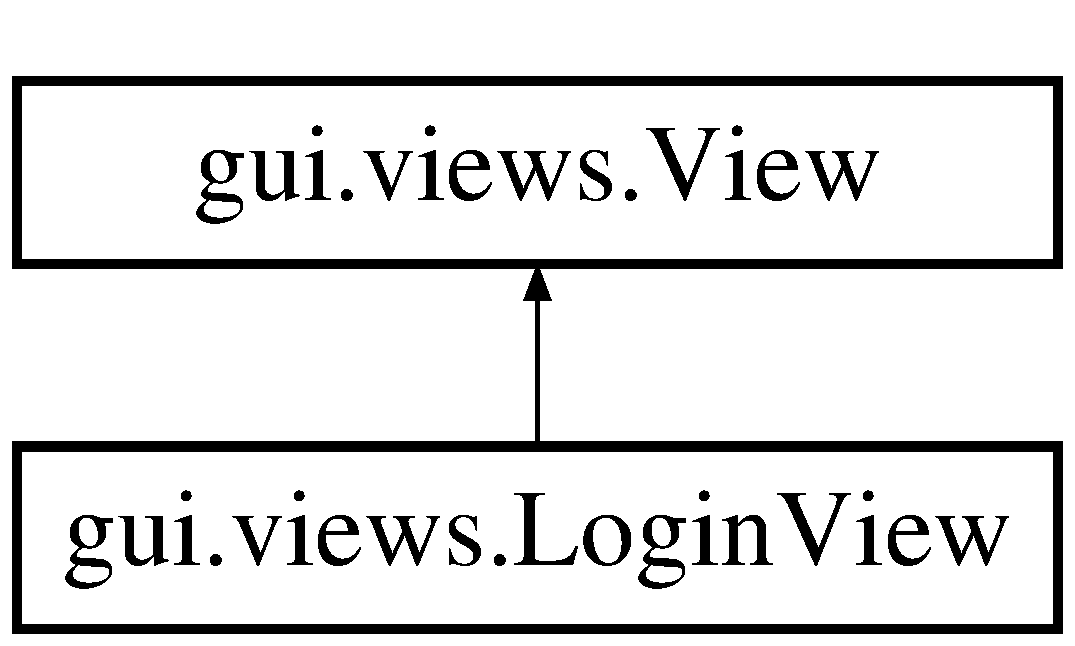
\includegraphics[height=2.000000cm]{classgui_1_1views_1_1_login_view}
\end{center}
\end{figure}
\subsection*{Public Member Functions}
\begin{DoxyCompactItemize}
\item 
\mbox{\hyperlink{classgui_1_1views_1_1_login_view_a0dfea90f88e5a83dadc2a4e6574ef6f3}{Login\+View}} (Container display)
\item 
String \mbox{\hyperlink{classgui_1_1views_1_1_login_view_af4b196f0c4956bd079e4f6c14e575ff8}{get\+Name}} ()
\end{DoxyCompactItemize}
\subsection*{Additional Inherited Members}


\subsection{Constructor \& Destructor Documentation}
\mbox{\Hypertarget{classgui_1_1views_1_1_login_view_a0dfea90f88e5a83dadc2a4e6574ef6f3}\label{classgui_1_1views_1_1_login_view_a0dfea90f88e5a83dadc2a4e6574ef6f3}} 
\index{gui\+::views\+::\+Login\+View@{gui\+::views\+::\+Login\+View}!Login\+View@{Login\+View}}
\index{Login\+View@{Login\+View}!gui\+::views\+::\+Login\+View@{gui\+::views\+::\+Login\+View}}
\subsubsection{\texorpdfstring{Login\+View()}{LoginView()}}
{\footnotesize\ttfamily gui.\+views.\+Login\+View.\+Login\+View (\begin{DoxyParamCaption}\item[{Container}]{display }\end{DoxyParamCaption})\hspace{0.3cm}{\ttfamily [inline]}}

Basic constructor, set components 
\begin{DoxyParams}{Parameters}
{\em display} & -\/ Container from actual frame \\
\hline
\end{DoxyParams}


\subsection{Member Function Documentation}
\mbox{\Hypertarget{classgui_1_1views_1_1_login_view_af4b196f0c4956bd079e4f6c14e575ff8}\label{classgui_1_1views_1_1_login_view_af4b196f0c4956bd079e4f6c14e575ff8}} 
\index{gui\+::views\+::\+Login\+View@{gui\+::views\+::\+Login\+View}!get\+Name@{get\+Name}}
\index{get\+Name@{get\+Name}!gui\+::views\+::\+Login\+View@{gui\+::views\+::\+Login\+View}}
\subsubsection{\texorpdfstring{get\+Name()}{getName()}}
{\footnotesize\ttfamily String gui.\+views.\+Login\+View.\+get\+Name (\begin{DoxyParamCaption}{ }\end{DoxyParamCaption})\hspace{0.3cm}{\ttfamily [inline]}}

\begin{DoxySeeAlso}{See also}
\mbox{\hyperlink{classgui_1_1views_1_1_view}{View}} 
\end{DoxySeeAlso}


The documentation for this class was generated from the following file\+:\begin{DoxyCompactItemize}
\item 
gui/views/Login\+View.\+java\end{DoxyCompactItemize}

\hypertarget{class_testing_1_1_main}{}\section{Testing.\+Main Class Reference}
\label{class_testing_1_1_main}\index{Testing.\+Main@{Testing.\+Main}}
\subsection*{Static Public Member Functions}
\begin{DoxyCompactItemize}
\item 
\mbox{\Hypertarget{class_testing_1_1_main_a1f0eb515fa1b5d53d7b4e66dc6ff4625}\label{class_testing_1_1_main_a1f0eb515fa1b5d53d7b4e66dc6ff4625}} 
static void {\bfseries main} (String\mbox{[}$\,$\mbox{]} args)  throws Class\+Not\+Found\+Exception, I\+O\+Exception, Data\+Card\+Exception 
\end{DoxyCompactItemize}


The documentation for this class was generated from the following file\+:\begin{DoxyCompactItemize}
\item 
Testing/Main.\+java\end{DoxyCompactItemize}

\hypertarget{classsystem_1_1exceptions_1_1_person_doesnt_exist_exception}{}\section{system.\+exceptions.\+Person\+Doesnt\+Exist\+Exception Class Reference}
\label{classsystem_1_1exceptions_1_1_person_doesnt_exist_exception}\index{system.\+exceptions.\+Person\+Doesnt\+Exist\+Exception@{system.\+exceptions.\+Person\+Doesnt\+Exist\+Exception}}
Inheritance diagram for system.\+exceptions.\+Person\+Doesnt\+Exist\+Exception\+:\begin{figure}[H]
\begin{center}
\leavevmode
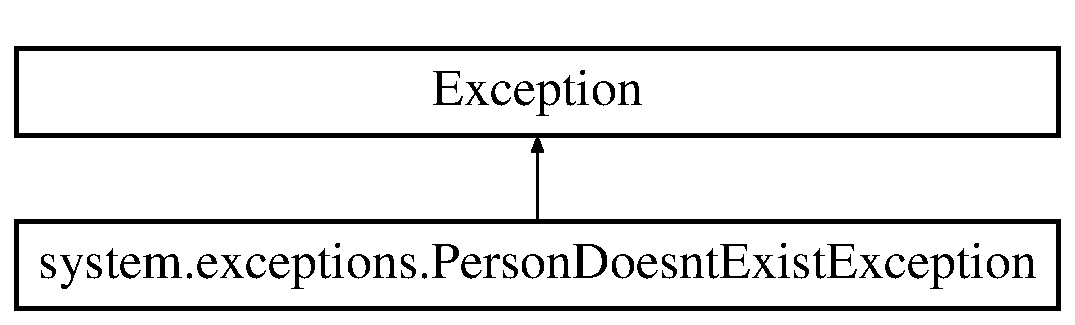
\includegraphics[height=2.000000cm]{classsystem_1_1exceptions_1_1_person_doesnt_exist_exception}
\end{center}
\end{figure}


The documentation for this class was generated from the following file\+:\begin{DoxyCompactItemize}
\item 
system/exceptions/Person\+Doesnt\+Exist\+Exception.\+java\end{DoxyCompactItemize}

\hypertarget{classmodules_1_1company_1_1_service_company}{}\section{modules.\+company.\+Service\+Company Class Reference}
\label{classmodules_1_1company_1_1_service_company}\index{modules.\+company.\+Service\+Company@{modules.\+company.\+Service\+Company}}
Inheritance diagram for modules.\+company.\+Service\+Company\+:\begin{figure}[H]
\begin{center}
\leavevmode
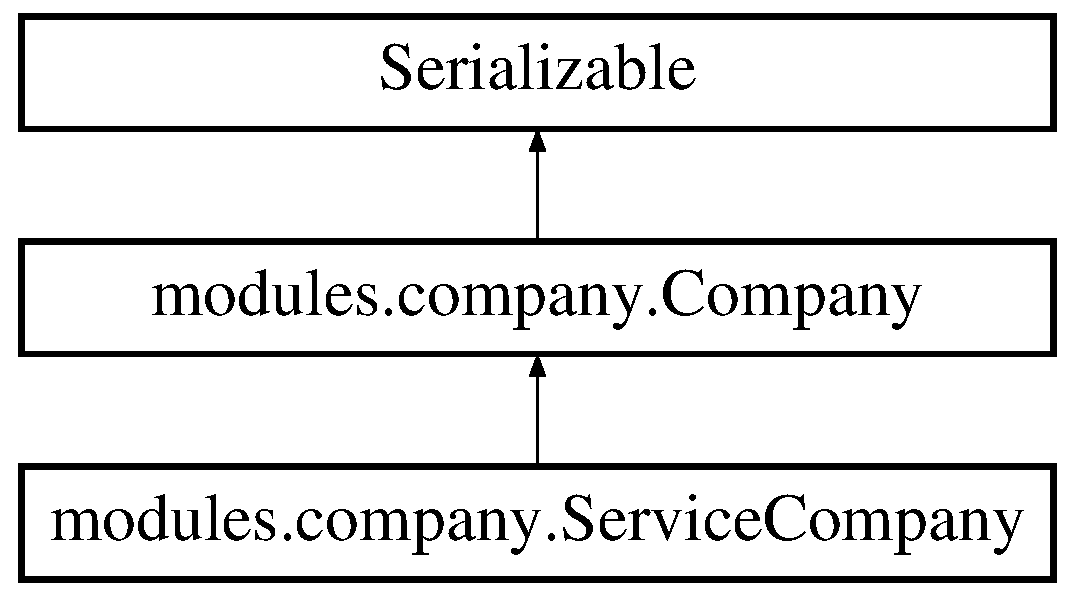
\includegraphics[height=3.000000cm]{classmodules_1_1company_1_1_service_company}
\end{center}
\end{figure}
\subsection*{Public Member Functions}
\begin{DoxyCompactItemize}
\item 
\mbox{\hyperlink{classmodules_1_1company_1_1_service_company_a63307bf3b961612ef5edaab613e0a1d5}{Service\+Company}} (String name)
\end{DoxyCompactItemize}
\subsection*{Additional Inherited Members}


\subsection{Detailed Description}
One type of the centrum client \begin{DoxyAuthor}{Author}
Micha� Fi�oczuk 
\end{DoxyAuthor}


\subsection{Constructor \& Destructor Documentation}
\mbox{\Hypertarget{classmodules_1_1company_1_1_service_company_a63307bf3b961612ef5edaab613e0a1d5}\label{classmodules_1_1company_1_1_service_company_a63307bf3b961612ef5edaab613e0a1d5}} 
\index{modules\+::company\+::\+Service\+Company@{modules\+::company\+::\+Service\+Company}!Service\+Company@{Service\+Company}}
\index{Service\+Company@{Service\+Company}!modules\+::company\+::\+Service\+Company@{modules\+::company\+::\+Service\+Company}}
\subsubsection{\texorpdfstring{Service\+Company()}{ServiceCompany()}}
{\footnotesize\ttfamily modules.\+company.\+Service\+Company.\+Service\+Company (\begin{DoxyParamCaption}\item[{String}]{name }\end{DoxyParamCaption})\hspace{0.3cm}{\ttfamily [inline]}}

Standard way to create service company 
\begin{DoxyParams}{Parameters}
{\em id} & long -\/number id of the company \\
\hline
{\em name} & String -\/ name of the \mbox{\hyperlink{classmodules_1_1company_1_1_company}{Company}} \\
\hline
\end{DoxyParams}


The documentation for this class was generated from the following file\+:\begin{DoxyCompactItemize}
\item 
modules/company/Service\+Company.\+java\end{DoxyCompactItemize}

\hypertarget{classmodules_1_1company_1_1_shop_company}{}\section{modules.\+company.\+Shop\+Company Class Reference}
\label{classmodules_1_1company_1_1_shop_company}\index{modules.\+company.\+Shop\+Company@{modules.\+company.\+Shop\+Company}}
Inheritance diagram for modules.\+company.\+Shop\+Company\+:\begin{figure}[H]
\begin{center}
\leavevmode
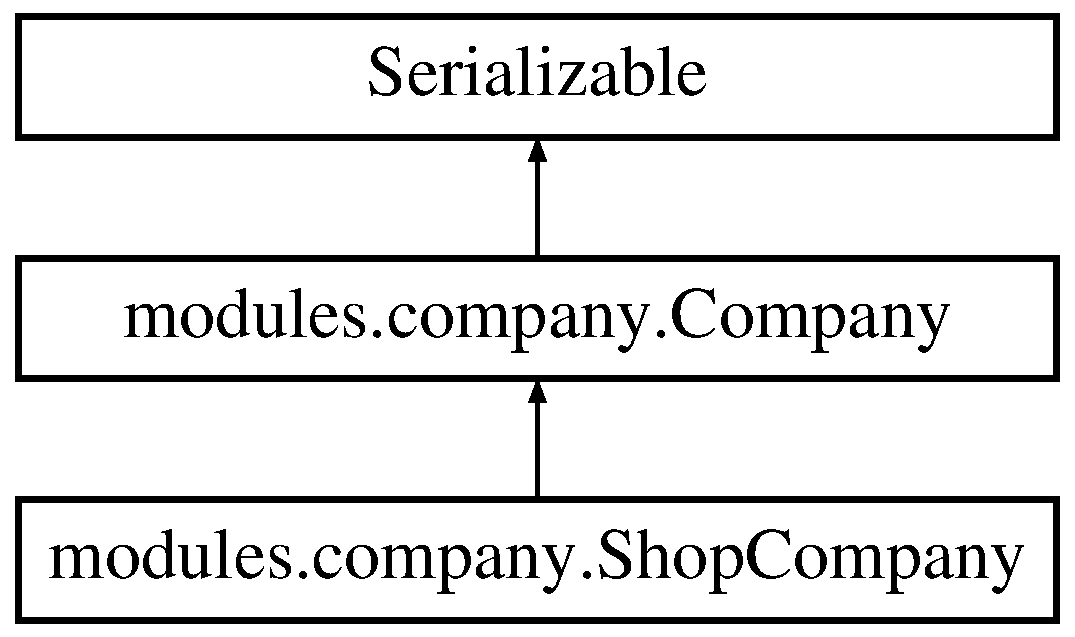
\includegraphics[height=3.000000cm]{classmodules_1_1company_1_1_shop_company}
\end{center}
\end{figure}
\subsection*{Public Member Functions}
\begin{DoxyCompactItemize}
\item 
\mbox{\hyperlink{classmodules_1_1company_1_1_shop_company_a678e2f71ffbb06efe5e1f02ef91a050b}{Shop\+Company}} (String name)
\end{DoxyCompactItemize}
\subsection*{Additional Inherited Members}


\subsection{Detailed Description}
One type of the centrum client \begin{DoxyAuthor}{Author}
Micha� Fi�o�czuk 
\end{DoxyAuthor}


\subsection{Constructor \& Destructor Documentation}
\mbox{\Hypertarget{classmodules_1_1company_1_1_shop_company_a678e2f71ffbb06efe5e1f02ef91a050b}\label{classmodules_1_1company_1_1_shop_company_a678e2f71ffbb06efe5e1f02ef91a050b}} 
\index{modules\+::company\+::\+Shop\+Company@{modules\+::company\+::\+Shop\+Company}!Shop\+Company@{Shop\+Company}}
\index{Shop\+Company@{Shop\+Company}!modules\+::company\+::\+Shop\+Company@{modules\+::company\+::\+Shop\+Company}}
\subsubsection{\texorpdfstring{Shop\+Company()}{ShopCompany()}}
{\footnotesize\ttfamily modules.\+company.\+Shop\+Company.\+Shop\+Company (\begin{DoxyParamCaption}\item[{String}]{name }\end{DoxyParamCaption})\hspace{0.3cm}{\ttfamily [inline]}}

Standard way to create shop company 
\begin{DoxyParams}{Parameters}
{\em id} & long-\/ id of the company \\
\hline
{\em name} & String -\/name of the company \\
\hline
\end{DoxyParams}


The documentation for this class was generated from the following file\+:\begin{DoxyCompactItemize}
\item 
modules/company/Shop\+Company.\+java\end{DoxyCompactItemize}

\hypertarget{classsystem_1_1exceptions_1_1_surname_exception}{}\section{system.\+exceptions.\+Surname\+Exception Class Reference}
\label{classsystem_1_1exceptions_1_1_surname_exception}\index{system.\+exceptions.\+Surname\+Exception@{system.\+exceptions.\+Surname\+Exception}}
Inheritance diagram for system.\+exceptions.\+Surname\+Exception\+:\begin{figure}[H]
\begin{center}
\leavevmode
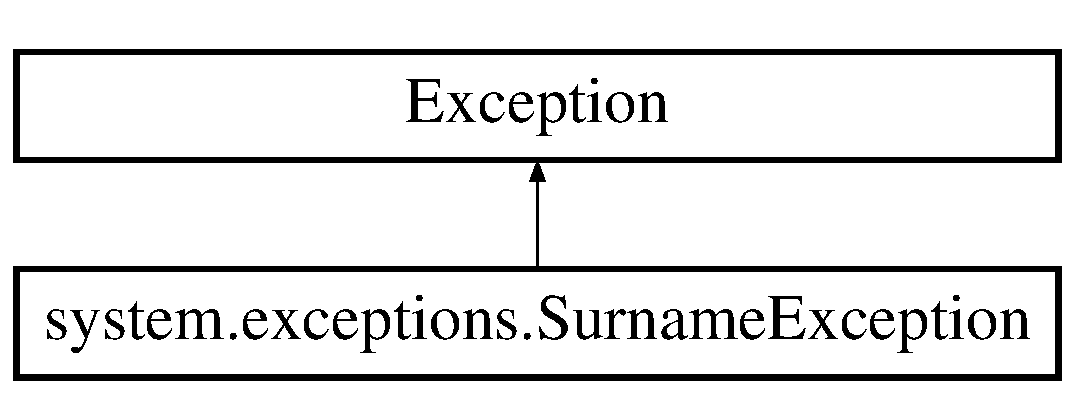
\includegraphics[height=2.000000cm]{classsystem_1_1exceptions_1_1_surname_exception}
\end{center}
\end{figure}


\subsection{Detailed Description}
Checks if surname have digits \begin{DoxyAuthor}{Author}
Ernest Stachelski 
\end{DoxyAuthor}
\begin{DoxyVersion}{Version}
0.\+1 
\end{DoxyVersion}


The documentation for this class was generated from the following file\+:\begin{DoxyCompactItemize}
\item 
system/exceptions/Surname\+Exception.\+java\end{DoxyCompactItemize}

\hypertarget{classmodules_1_1center_1_1_transaction}{}\section{modules.\+center.\+Transaction Class Reference}
\label{classmodules_1_1center_1_1_transaction}\index{modules.\+center.\+Transaction@{modules.\+center.\+Transaction}}
Inheritance diagram for modules.\+center.\+Transaction\+:\begin{figure}[H]
\begin{center}
\leavevmode
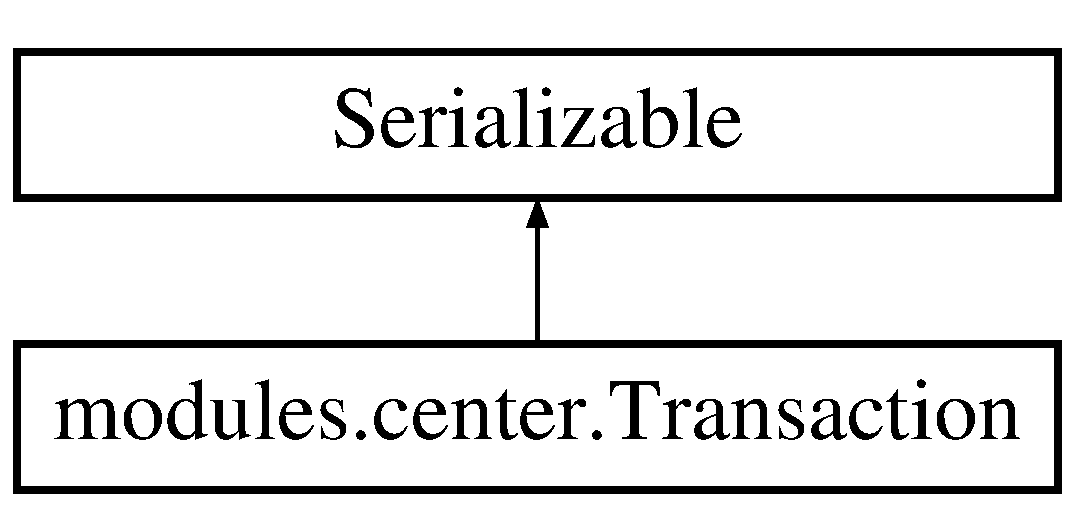
\includegraphics[height=2.000000cm]{classmodules_1_1center_1_1_transaction}
\end{center}
\end{figure}
\subsection*{Public Member Functions}
\begin{DoxyCompactItemize}
\item 
\mbox{\hyperlink{classmodules_1_1center_1_1_transaction_a9c2f6911a50a48045ae02cf3745ab099}{Transaction}} (\mbox{\hyperlink{classmodules_1_1company_1_1_company}{Company}} comp, \mbox{\hyperlink{classmodules_1_1bank_1_1_bank}{Bank}} bank, \mbox{\hyperlink{classmodules_1_1bank_1_1_card}{Card}} card, double amount, String date)
\item 
\mbox{\hyperlink{classmodules_1_1company_1_1_company}{Company}} \mbox{\hyperlink{classmodules_1_1center_1_1_transaction_a36736cde43af28fdbdbd8f654c06f43f}{get\+Comp}} ()
\item 
void \mbox{\hyperlink{classmodules_1_1center_1_1_transaction_a64eefb348cd04298f7ce558520ade5c1}{set\+Comp}} (\mbox{\hyperlink{classmodules_1_1company_1_1_company}{Company}} comp)
\item 
\mbox{\hyperlink{classmodules_1_1bank_1_1_card}{Card}} \mbox{\hyperlink{classmodules_1_1center_1_1_transaction_a4e88acd3f3e8c57b607f1a530d0b20e9}{get\+Card}} ()
\item 
void \mbox{\hyperlink{classmodules_1_1center_1_1_transaction_a58f60b56607132a4c4f7e3b600678c62}{set\+Card}} (\mbox{\hyperlink{classmodules_1_1bank_1_1_card}{Card}} card)
\item 
double \mbox{\hyperlink{classmodules_1_1center_1_1_transaction_a07f5da80f0513a62a446af3cd920a060}{get\+Amount}} ()
\item 
void \mbox{\hyperlink{classmodules_1_1center_1_1_transaction_a691012713b25759ed7b766dbc5d47ed8}{set\+Amount}} (double amount)
\item 
String \mbox{\hyperlink{classmodules_1_1center_1_1_transaction_a4a1d002cbca929b11c9e6b85308b9f9b}{get\+Date}} ()
\item 
void \mbox{\hyperlink{classmodules_1_1center_1_1_transaction_a7c47993064afc6b1eb49c04c5e3021a4}{set\+Date}} (String date)
\item 
\mbox{\hyperlink{classmodules_1_1bank_1_1_bank}{Bank}} \mbox{\hyperlink{classmodules_1_1center_1_1_transaction_abf7f185bbd1e2843e269630b01b15d49}{get\+Bank}} ()
\item 
void \mbox{\hyperlink{classmodules_1_1center_1_1_transaction_a526239006b95c701732c22125ea7badc}{set\+Bank}} (\mbox{\hyperlink{classmodules_1_1bank_1_1_bank}{Bank}} bank)
\item 
String \mbox{\hyperlink{classmodules_1_1center_1_1_transaction_a05507271a0e2347ee6c555cf39fc232e}{to\+String}} ()
\end{DoxyCompactItemize}


\subsection{Detailed Description}
The properties of transaction that were created in the company,contains the object of company, object of the card, amount and date.

\begin{DoxyAuthor}{Author}
Micha� Fi�o�czuk 
\end{DoxyAuthor}
\begin{DoxyVersion}{Version}
0.\+5 
\end{DoxyVersion}


\subsection{Constructor \& Destructor Documentation}
\mbox{\Hypertarget{classmodules_1_1center_1_1_transaction_a9c2f6911a50a48045ae02cf3745ab099}\label{classmodules_1_1center_1_1_transaction_a9c2f6911a50a48045ae02cf3745ab099}} 
\index{modules\+::center\+::\+Transaction@{modules\+::center\+::\+Transaction}!Transaction@{Transaction}}
\index{Transaction@{Transaction}!modules\+::center\+::\+Transaction@{modules\+::center\+::\+Transaction}}
\subsubsection{\texorpdfstring{Transaction()}{Transaction()}}
{\footnotesize\ttfamily modules.\+center.\+Transaction.\+Transaction (\begin{DoxyParamCaption}\item[{\mbox{\hyperlink{classmodules_1_1company_1_1_company}{Company}}}]{comp,  }\item[{\mbox{\hyperlink{classmodules_1_1bank_1_1_bank}{Bank}}}]{bank,  }\item[{\mbox{\hyperlink{classmodules_1_1bank_1_1_card}{Card}}}]{card,  }\item[{double}]{amount,  }\item[{String}]{date }\end{DoxyParamCaption})\hspace{0.3cm}{\ttfamily [inline]}}

Standard way to create transaction object with filled fields 
\begin{DoxyParams}{Parameters}
{\em comp} & object of the company where transaction was created \\
\hline
{\em card} & object of the card that was used in transation \\
\hline
{\em amount} & value of the transaction \\
\hline
{\em date} & date of the transaction \\
\hline
\end{DoxyParams}


\subsection{Member Function Documentation}
\mbox{\Hypertarget{classmodules_1_1center_1_1_transaction_a07f5da80f0513a62a446af3cd920a060}\label{classmodules_1_1center_1_1_transaction_a07f5da80f0513a62a446af3cd920a060}} 
\index{modules\+::center\+::\+Transaction@{modules\+::center\+::\+Transaction}!get\+Amount@{get\+Amount}}
\index{get\+Amount@{get\+Amount}!modules\+::center\+::\+Transaction@{modules\+::center\+::\+Transaction}}
\subsubsection{\texorpdfstring{get\+Amount()}{getAmount()}}
{\footnotesize\ttfamily double modules.\+center.\+Transaction.\+get\+Amount (\begin{DoxyParamCaption}{ }\end{DoxyParamCaption})\hspace{0.3cm}{\ttfamily [inline]}}

Gets amount of money used in this transaction \begin{DoxyReturn}{Returns}
double value 
\end{DoxyReturn}
\mbox{\Hypertarget{classmodules_1_1center_1_1_transaction_abf7f185bbd1e2843e269630b01b15d49}\label{classmodules_1_1center_1_1_transaction_abf7f185bbd1e2843e269630b01b15d49}} 
\index{modules\+::center\+::\+Transaction@{modules\+::center\+::\+Transaction}!get\+Bank@{get\+Bank}}
\index{get\+Bank@{get\+Bank}!modules\+::center\+::\+Transaction@{modules\+::center\+::\+Transaction}}
\subsubsection{\texorpdfstring{get\+Bank()}{getBank()}}
{\footnotesize\ttfamily \mbox{\hyperlink{classmodules_1_1bank_1_1_bank}{Bank}} modules.\+center.\+Transaction.\+get\+Bank (\begin{DoxyParamCaption}{ }\end{DoxyParamCaption})\hspace{0.3cm}{\ttfamily [inline]}}

Gets bank connected with this transaction \begin{DoxyReturn}{Returns}
Bank object 
\end{DoxyReturn}
\mbox{\Hypertarget{classmodules_1_1center_1_1_transaction_a4e88acd3f3e8c57b607f1a530d0b20e9}\label{classmodules_1_1center_1_1_transaction_a4e88acd3f3e8c57b607f1a530d0b20e9}} 
\index{modules\+::center\+::\+Transaction@{modules\+::center\+::\+Transaction}!get\+Card@{get\+Card}}
\index{get\+Card@{get\+Card}!modules\+::center\+::\+Transaction@{modules\+::center\+::\+Transaction}}
\subsubsection{\texorpdfstring{get\+Card()}{getCard()}}
{\footnotesize\ttfamily \mbox{\hyperlink{classmodules_1_1bank_1_1_card}{Card}} modules.\+center.\+Transaction.\+get\+Card (\begin{DoxyParamCaption}{ }\end{DoxyParamCaption})\hspace{0.3cm}{\ttfamily [inline]}}

Gets card connected with this transaction \begin{DoxyReturn}{Returns}
Credit\+Card, Bank\+Card or Debit\+Card object 
\end{DoxyReturn}
\mbox{\Hypertarget{classmodules_1_1center_1_1_transaction_a36736cde43af28fdbdbd8f654c06f43f}\label{classmodules_1_1center_1_1_transaction_a36736cde43af28fdbdbd8f654c06f43f}} 
\index{modules\+::center\+::\+Transaction@{modules\+::center\+::\+Transaction}!get\+Comp@{get\+Comp}}
\index{get\+Comp@{get\+Comp}!modules\+::center\+::\+Transaction@{modules\+::center\+::\+Transaction}}
\subsubsection{\texorpdfstring{get\+Comp()}{getComp()}}
{\footnotesize\ttfamily \mbox{\hyperlink{classmodules_1_1company_1_1_company}{Company}} modules.\+center.\+Transaction.\+get\+Comp (\begin{DoxyParamCaption}{ }\end{DoxyParamCaption})\hspace{0.3cm}{\ttfamily [inline]}}

Gets company connected with this transaction \begin{DoxyReturn}{Returns}
Company object 
\end{DoxyReturn}
\mbox{\Hypertarget{classmodules_1_1center_1_1_transaction_a4a1d002cbca929b11c9e6b85308b9f9b}\label{classmodules_1_1center_1_1_transaction_a4a1d002cbca929b11c9e6b85308b9f9b}} 
\index{modules\+::center\+::\+Transaction@{modules\+::center\+::\+Transaction}!get\+Date@{get\+Date}}
\index{get\+Date@{get\+Date}!modules\+::center\+::\+Transaction@{modules\+::center\+::\+Transaction}}
\subsubsection{\texorpdfstring{get\+Date()}{getDate()}}
{\footnotesize\ttfamily String modules.\+center.\+Transaction.\+get\+Date (\begin{DoxyParamCaption}{ }\end{DoxyParamCaption})\hspace{0.3cm}{\ttfamily [inline]}}

Gets date of the transaction \begin{DoxyReturn}{Returns}
String date in format \char`\"{}\+Y\+Y\+Y\+Y-\/\+M\+M-\/\+D\+D\char`\"{} 
\end{DoxyReturn}
\mbox{\Hypertarget{classmodules_1_1center_1_1_transaction_a691012713b25759ed7b766dbc5d47ed8}\label{classmodules_1_1center_1_1_transaction_a691012713b25759ed7b766dbc5d47ed8}} 
\index{modules\+::center\+::\+Transaction@{modules\+::center\+::\+Transaction}!set\+Amount@{set\+Amount}}
\index{set\+Amount@{set\+Amount}!modules\+::center\+::\+Transaction@{modules\+::center\+::\+Transaction}}
\subsubsection{\texorpdfstring{set\+Amount()}{setAmount()}}
{\footnotesize\ttfamily void modules.\+center.\+Transaction.\+set\+Amount (\begin{DoxyParamCaption}\item[{double}]{amount }\end{DoxyParamCaption})\hspace{0.3cm}{\ttfamily [inline]}}

Sets amount of money used in this transaction 
\begin{DoxyParams}{Parameters}
{\em amount} & -\/ double value \\
\hline
\end{DoxyParams}
\mbox{\Hypertarget{classmodules_1_1center_1_1_transaction_a526239006b95c701732c22125ea7badc}\label{classmodules_1_1center_1_1_transaction_a526239006b95c701732c22125ea7badc}} 
\index{modules\+::center\+::\+Transaction@{modules\+::center\+::\+Transaction}!set\+Bank@{set\+Bank}}
\index{set\+Bank@{set\+Bank}!modules\+::center\+::\+Transaction@{modules\+::center\+::\+Transaction}}
\subsubsection{\texorpdfstring{set\+Bank()}{setBank()}}
{\footnotesize\ttfamily void modules.\+center.\+Transaction.\+set\+Bank (\begin{DoxyParamCaption}\item[{\mbox{\hyperlink{classmodules_1_1bank_1_1_bank}{Bank}}}]{bank }\end{DoxyParamCaption})\hspace{0.3cm}{\ttfamily [inline]}}

Sets bank connected with this transaction \mbox{\Hypertarget{classmodules_1_1center_1_1_transaction_a58f60b56607132a4c4f7e3b600678c62}\label{classmodules_1_1center_1_1_transaction_a58f60b56607132a4c4f7e3b600678c62}} 
\index{modules\+::center\+::\+Transaction@{modules\+::center\+::\+Transaction}!set\+Card@{set\+Card}}
\index{set\+Card@{set\+Card}!modules\+::center\+::\+Transaction@{modules\+::center\+::\+Transaction}}
\subsubsection{\texorpdfstring{set\+Card()}{setCard()}}
{\footnotesize\ttfamily void modules.\+center.\+Transaction.\+set\+Card (\begin{DoxyParamCaption}\item[{\mbox{\hyperlink{classmodules_1_1bank_1_1_card}{Card}}}]{card }\end{DoxyParamCaption})\hspace{0.3cm}{\ttfamily [inline]}}

Sets card connected with this transaction 
\begin{DoxyParams}{Parameters}
{\em card} & -\/ specified type of card to bind \\
\hline
\end{DoxyParams}
\mbox{\Hypertarget{classmodules_1_1center_1_1_transaction_a64eefb348cd04298f7ce558520ade5c1}\label{classmodules_1_1center_1_1_transaction_a64eefb348cd04298f7ce558520ade5c1}} 
\index{modules\+::center\+::\+Transaction@{modules\+::center\+::\+Transaction}!set\+Comp@{set\+Comp}}
\index{set\+Comp@{set\+Comp}!modules\+::center\+::\+Transaction@{modules\+::center\+::\+Transaction}}
\subsubsection{\texorpdfstring{set\+Comp()}{setComp()}}
{\footnotesize\ttfamily void modules.\+center.\+Transaction.\+set\+Comp (\begin{DoxyParamCaption}\item[{\mbox{\hyperlink{classmodules_1_1company_1_1_company}{Company}}}]{comp }\end{DoxyParamCaption})\hspace{0.3cm}{\ttfamily [inline]}}

Sets company connected with this transaction 
\begin{DoxyParams}{Parameters}
{\em comp} & -\/ company object \\
\hline
\end{DoxyParams}
\mbox{\Hypertarget{classmodules_1_1center_1_1_transaction_a7c47993064afc6b1eb49c04c5e3021a4}\label{classmodules_1_1center_1_1_transaction_a7c47993064afc6b1eb49c04c5e3021a4}} 
\index{modules\+::center\+::\+Transaction@{modules\+::center\+::\+Transaction}!set\+Date@{set\+Date}}
\index{set\+Date@{set\+Date}!modules\+::center\+::\+Transaction@{modules\+::center\+::\+Transaction}}
\subsubsection{\texorpdfstring{set\+Date()}{setDate()}}
{\footnotesize\ttfamily void modules.\+center.\+Transaction.\+set\+Date (\begin{DoxyParamCaption}\item[{String}]{date }\end{DoxyParamCaption})\hspace{0.3cm}{\ttfamily [inline]}}

Sets date of the transaction 
\begin{DoxyParams}{Parameters}
{\em date} & -\/ string in format \char`\"{}\+Y\+Y\+Y\+Y-\/\+M\+M-\/\+D\+D\char`\"{} \\
\hline
\end{DoxyParams}
\mbox{\Hypertarget{classmodules_1_1center_1_1_transaction_a05507271a0e2347ee6c555cf39fc232e}\label{classmodules_1_1center_1_1_transaction_a05507271a0e2347ee6c555cf39fc232e}} 
\index{modules\+::center\+::\+Transaction@{modules\+::center\+::\+Transaction}!to\+String@{to\+String}}
\index{to\+String@{to\+String}!modules\+::center\+::\+Transaction@{modules\+::center\+::\+Transaction}}
\subsubsection{\texorpdfstring{to\+String()}{toString()}}
{\footnotesize\ttfamily String modules.\+center.\+Transaction.\+to\+String (\begin{DoxyParamCaption}{ }\end{DoxyParamCaption})\hspace{0.3cm}{\ttfamily [inline]}}

Converts object to string value 

The documentation for this class was generated from the following file\+:\begin{DoxyCompactItemize}
\item 
modules/center/Transaction.\+java\end{DoxyCompactItemize}

\hypertarget{classmodules_1_1company_1_1_transport_company}{}\section{modules.\+company.\+Transport\+Company Class Reference}
\label{classmodules_1_1company_1_1_transport_company}\index{modules.\+company.\+Transport\+Company@{modules.\+company.\+Transport\+Company}}
Inheritance diagram for modules.\+company.\+Transport\+Company\+:\begin{figure}[H]
\begin{center}
\leavevmode
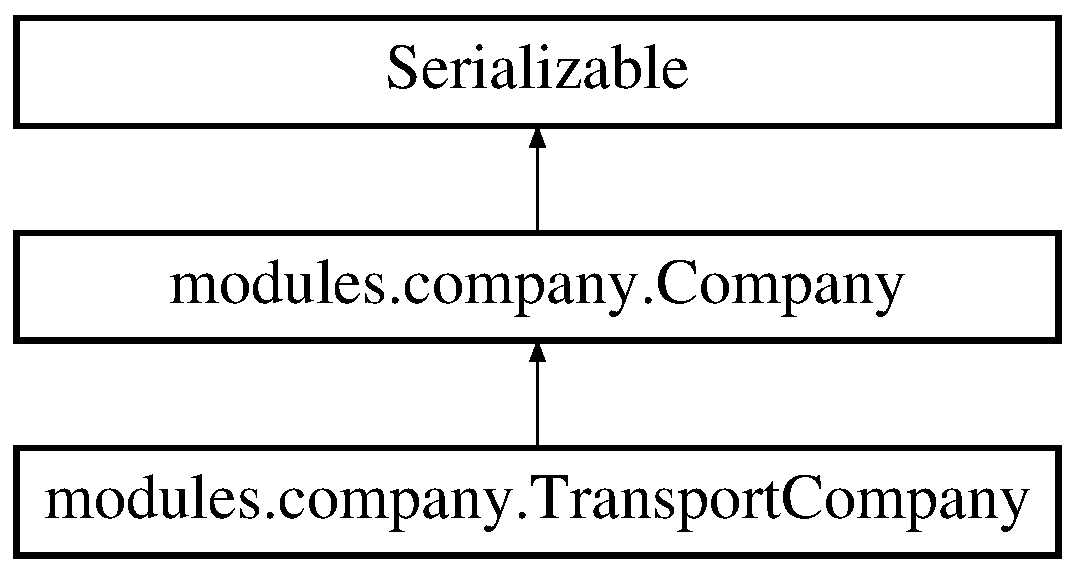
\includegraphics[height=3.000000cm]{classmodules_1_1company_1_1_transport_company}
\end{center}
\end{figure}
\subsection*{Public Member Functions}
\begin{DoxyCompactItemize}
\item 
\mbox{\hyperlink{classmodules_1_1company_1_1_transport_company_a03e706b8bcf1306b3ad9fbdd1250d196}{Transport\+Company}} (String name)
\end{DoxyCompactItemize}
\subsection*{Additional Inherited Members}


\subsection{Detailed Description}
One type of the \mbox{\hyperlink{classmodules_1_1company_1_1_company}{Company}} \begin{DoxyAuthor}{Author}
Micha� Fi�o�czuk 
\end{DoxyAuthor}


\subsection{Constructor \& Destructor Documentation}
\mbox{\Hypertarget{classmodules_1_1company_1_1_transport_company_a03e706b8bcf1306b3ad9fbdd1250d196}\label{classmodules_1_1company_1_1_transport_company_a03e706b8bcf1306b3ad9fbdd1250d196}} 
\index{modules\+::company\+::\+Transport\+Company@{modules\+::company\+::\+Transport\+Company}!Transport\+Company@{Transport\+Company}}
\index{Transport\+Company@{Transport\+Company}!modules\+::company\+::\+Transport\+Company@{modules\+::company\+::\+Transport\+Company}}
\subsubsection{\texorpdfstring{Transport\+Company()}{TransportCompany()}}
{\footnotesize\ttfamily modules.\+company.\+Transport\+Company.\+Transport\+Company (\begin{DoxyParamCaption}\item[{String}]{name }\end{DoxyParamCaption})\hspace{0.3cm}{\ttfamily [inline]}}

Standard way to transport company 
\begin{DoxyParams}{Parameters}
{\em id} & long -\/id of the company \\
\hline
{\em name} & String-\/ name of the company \\
\hline
\end{DoxyParams}


The documentation for this class was generated from the following file\+:\begin{DoxyCompactItemize}
\item 
modules/company/Transport\+Company.\+java\end{DoxyCompactItemize}

\hypertarget{classmodules_1_1center_1_1_user}{}\section{modules.\+center.\+User Class Reference}
\label{classmodules_1_1center_1_1_user}\index{modules.\+center.\+User@{modules.\+center.\+User}}
Inheritance diagram for modules.\+center.\+User\+:\begin{figure}[H]
\begin{center}
\leavevmode
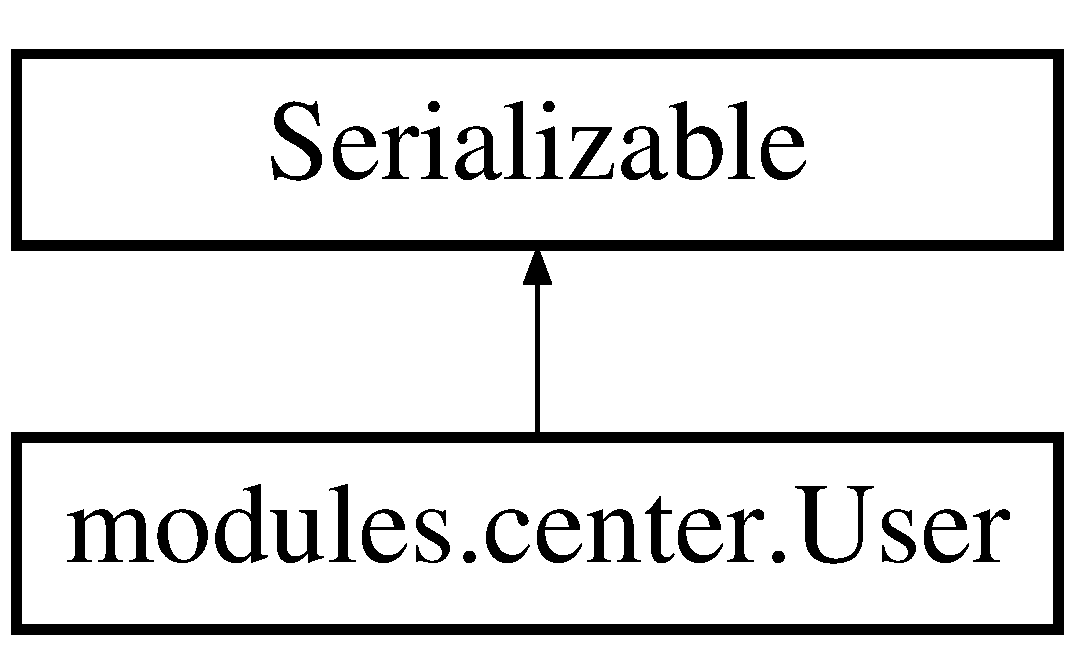
\includegraphics[height=2.000000cm]{classmodules_1_1center_1_1_user}
\end{center}
\end{figure}
\subsection*{Public Member Functions}
\begin{DoxyCompactItemize}
\item 
\mbox{\hyperlink{classmodules_1_1center_1_1_user_a278edac53aa5b305a85b0c4023c8b141}{User}} (String login, String password, String rights, String org\+Name)
\item 
String \mbox{\hyperlink{classmodules_1_1center_1_1_user_a1766cc2ff541a3087d621f96b773b7b7}{get\+Login}} ()
\item 
void \mbox{\hyperlink{classmodules_1_1center_1_1_user_a4b6a9c0c62c0e63dadaca94c72a7e45c}{set\+Login}} (String login)
\item 
String \mbox{\hyperlink{classmodules_1_1center_1_1_user_a1f9bdd70c1d53709fe12ca0d6cfef859}{get\+Password}} ()
\item 
void \mbox{\hyperlink{classmodules_1_1center_1_1_user_a6745b9f563ef2e5249f2caffbcd05f8f}{set\+Password}} (String password)
\item 
String \mbox{\hyperlink{classmodules_1_1center_1_1_user_a33af50e848713dc8811b4bb439e1dc29}{get\+Rights}} ()
\item 
void \mbox{\hyperlink{classmodules_1_1center_1_1_user_ad00308dfa5ef6aacf2778f4610b0b97a}{set\+Rights}} (String rights)
\item 
String \mbox{\hyperlink{classmodules_1_1center_1_1_user_a88070c518d2171398a86810a2e6112a2}{get\+Org\+Name}} ()
\end{DoxyCompactItemize}


\subsection{Detailed Description}
Class which represents the users of the center \begin{DoxyAuthor}{Author}
Fi�o�czuk Micha� 
\end{DoxyAuthor}
\begin{DoxyVersion}{Version}
0.\+5 
\end{DoxyVersion}


\subsection{Constructor \& Destructor Documentation}
\mbox{\Hypertarget{classmodules_1_1center_1_1_user_a278edac53aa5b305a85b0c4023c8b141}\label{classmodules_1_1center_1_1_user_a278edac53aa5b305a85b0c4023c8b141}} 
\index{modules\+::center\+::\+User@{modules\+::center\+::\+User}!User@{User}}
\index{User@{User}!modules\+::center\+::\+User@{modules\+::center\+::\+User}}
\subsubsection{\texorpdfstring{User()}{User()}}
{\footnotesize\ttfamily modules.\+center.\+User.\+User (\begin{DoxyParamCaption}\item[{String}]{login,  }\item[{String}]{password,  }\item[{String}]{rights,  }\item[{String}]{org\+Name }\end{DoxyParamCaption})\hspace{0.3cm}{\ttfamily [inline]}}

Standard way to create \mbox{\hyperlink{classmodules_1_1center_1_1_user}{User}} object 
\begin{DoxyParams}{Parameters}
{\em login} & -\/ String contains user\textquotesingle{}s login \\
\hline
{\em password} & -\/ String contains unencrypted password \\
\hline
{\em rights} & -\/ String contains one of the option from Combo\+Box in G\+UI\textquotesingle{}s language \\
\hline
{\em org\+Name} & -\/ String name of Bank or Company. If doesn\textquotesingle{}t exists put empty string \\
\hline
\end{DoxyParams}


\subsection{Member Function Documentation}
\mbox{\Hypertarget{classmodules_1_1center_1_1_user_a1766cc2ff541a3087d621f96b773b7b7}\label{classmodules_1_1center_1_1_user_a1766cc2ff541a3087d621f96b773b7b7}} 
\index{modules\+::center\+::\+User@{modules\+::center\+::\+User}!get\+Login@{get\+Login}}
\index{get\+Login@{get\+Login}!modules\+::center\+::\+User@{modules\+::center\+::\+User}}
\subsubsection{\texorpdfstring{get\+Login()}{getLogin()}}
{\footnotesize\ttfamily String modules.\+center.\+User.\+get\+Login (\begin{DoxyParamCaption}{ }\end{DoxyParamCaption})\hspace{0.3cm}{\ttfamily [inline]}}

Getter of the login \begin{DoxyReturn}{Returns}
String, login of the user 
\end{DoxyReturn}
\mbox{\Hypertarget{classmodules_1_1center_1_1_user_a88070c518d2171398a86810a2e6112a2}\label{classmodules_1_1center_1_1_user_a88070c518d2171398a86810a2e6112a2}} 
\index{modules\+::center\+::\+User@{modules\+::center\+::\+User}!get\+Org\+Name@{get\+Org\+Name}}
\index{get\+Org\+Name@{get\+Org\+Name}!modules\+::center\+::\+User@{modules\+::center\+::\+User}}
\subsubsection{\texorpdfstring{get\+Org\+Name()}{getOrgName()}}
{\footnotesize\ttfamily String modules.\+center.\+User.\+get\+Org\+Name (\begin{DoxyParamCaption}{ }\end{DoxyParamCaption})\hspace{0.3cm}{\ttfamily [inline]}}

Setter of the bank or company name \begin{DoxyReturn}{Returns}
String organisation name 
\end{DoxyReturn}
\mbox{\Hypertarget{classmodules_1_1center_1_1_user_a1f9bdd70c1d53709fe12ca0d6cfef859}\label{classmodules_1_1center_1_1_user_a1f9bdd70c1d53709fe12ca0d6cfef859}} 
\index{modules\+::center\+::\+User@{modules\+::center\+::\+User}!get\+Password@{get\+Password}}
\index{get\+Password@{get\+Password}!modules\+::center\+::\+User@{modules\+::center\+::\+User}}
\subsubsection{\texorpdfstring{get\+Password()}{getPassword()}}
{\footnotesize\ttfamily String modules.\+center.\+User.\+get\+Password (\begin{DoxyParamCaption}{ }\end{DoxyParamCaption})\hspace{0.3cm}{\ttfamily [inline]}}

Getter of the password of the user \begin{DoxyReturn}{Returns}
String,password of the user 
\end{DoxyReturn}
\mbox{\Hypertarget{classmodules_1_1center_1_1_user_a33af50e848713dc8811b4bb439e1dc29}\label{classmodules_1_1center_1_1_user_a33af50e848713dc8811b4bb439e1dc29}} 
\index{modules\+::center\+::\+User@{modules\+::center\+::\+User}!get\+Rights@{get\+Rights}}
\index{get\+Rights@{get\+Rights}!modules\+::center\+::\+User@{modules\+::center\+::\+User}}
\subsubsection{\texorpdfstring{get\+Rights()}{getRights()}}
{\footnotesize\ttfamily String modules.\+center.\+User.\+get\+Rights (\begin{DoxyParamCaption}{ }\end{DoxyParamCaption})\hspace{0.3cm}{\ttfamily [inline]}}

Getter of the rights of the user \begin{DoxyReturn}{Returns}
String, rights of the user 
\end{DoxyReturn}
\mbox{\Hypertarget{classmodules_1_1center_1_1_user_a4b6a9c0c62c0e63dadaca94c72a7e45c}\label{classmodules_1_1center_1_1_user_a4b6a9c0c62c0e63dadaca94c72a7e45c}} 
\index{modules\+::center\+::\+User@{modules\+::center\+::\+User}!set\+Login@{set\+Login}}
\index{set\+Login@{set\+Login}!modules\+::center\+::\+User@{modules\+::center\+::\+User}}
\subsubsection{\texorpdfstring{set\+Login()}{setLogin()}}
{\footnotesize\ttfamily void modules.\+center.\+User.\+set\+Login (\begin{DoxyParamCaption}\item[{String}]{login }\end{DoxyParamCaption})\hspace{0.3cm}{\ttfamily [inline]}}

Setter of the login 
\begin{DoxyParams}{Parameters}
{\em login} & String, new login of the user \\
\hline
\end{DoxyParams}
\mbox{\Hypertarget{classmodules_1_1center_1_1_user_a6745b9f563ef2e5249f2caffbcd05f8f}\label{classmodules_1_1center_1_1_user_a6745b9f563ef2e5249f2caffbcd05f8f}} 
\index{modules\+::center\+::\+User@{modules\+::center\+::\+User}!set\+Password@{set\+Password}}
\index{set\+Password@{set\+Password}!modules\+::center\+::\+User@{modules\+::center\+::\+User}}
\subsubsection{\texorpdfstring{set\+Password()}{setPassword()}}
{\footnotesize\ttfamily void modules.\+center.\+User.\+set\+Password (\begin{DoxyParamCaption}\item[{String}]{password }\end{DoxyParamCaption})\hspace{0.3cm}{\ttfamily [inline]}}

Setter of the password of the user 
\begin{DoxyParams}{Parameters}
{\em password} & String, new password of the user \\
\hline
\end{DoxyParams}
\mbox{\Hypertarget{classmodules_1_1center_1_1_user_ad00308dfa5ef6aacf2778f4610b0b97a}\label{classmodules_1_1center_1_1_user_ad00308dfa5ef6aacf2778f4610b0b97a}} 
\index{modules\+::center\+::\+User@{modules\+::center\+::\+User}!set\+Rights@{set\+Rights}}
\index{set\+Rights@{set\+Rights}!modules\+::center\+::\+User@{modules\+::center\+::\+User}}
\subsubsection{\texorpdfstring{set\+Rights()}{setRights()}}
{\footnotesize\ttfamily void modules.\+center.\+User.\+set\+Rights (\begin{DoxyParamCaption}\item[{String}]{rights }\end{DoxyParamCaption})\hspace{0.3cm}{\ttfamily [inline]}}

Setter of the rights of the user 
\begin{DoxyParams}{Parameters}
{\em rights} & String, new rights of user \\
\hline
\end{DoxyParams}


The documentation for this class was generated from the following file\+:\begin{DoxyCompactItemize}
\item 
modules/center/User.\+java\end{DoxyCompactItemize}

\hypertarget{classgui_1_1views_1_1_view}{}\section{gui.\+views.\+View Class Reference}
\label{classgui_1_1views_1_1_view}\index{gui.\+views.\+View@{gui.\+views.\+View}}
Inheritance diagram for gui.\+views.\+View\+:\begin{figure}[H]
\begin{center}
\leavevmode
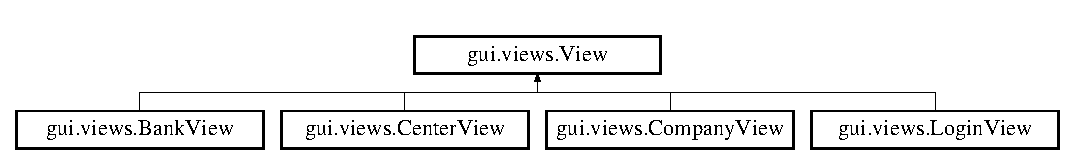
\includegraphics[height=1.772152cm]{classgui_1_1views_1_1_view}
\end{center}
\end{figure}
\subsection*{Public Member Functions}
\begin{DoxyCompactItemize}
\item 
\mbox{\Hypertarget{classgui_1_1views_1_1_view_a8484a1ea97e59db45fe8b9c5d87ee7cb}\label{classgui_1_1views_1_1_view_a8484a1ea97e59db45fe8b9c5d87ee7cb}} 
{\bfseries View} (Container display)
\item 
\mbox{\Hypertarget{classgui_1_1views_1_1_view_a44966bc8962ce254d54b6378caa06460}\label{classgui_1_1views_1_1_view_a44966bc8962ce254d54b6378caa06460}} 
J\+Panel {\bfseries get\+Panel} ()
\item 
\mbox{\Hypertarget{classgui_1_1views_1_1_view_a3cdad1416bdab94eeecb54edef240c61}\label{classgui_1_1views_1_1_view_a3cdad1416bdab94eeecb54edef240c61}} 
abstract String {\bfseries get\+Name} ()
\end{DoxyCompactItemize}
\subsection*{Protected Attributes}
\begin{DoxyCompactItemize}
\item 
\mbox{\Hypertarget{classgui_1_1views_1_1_view_a7c42ea37c4adb29a4a6fa3ccdf1eda3a}\label{classgui_1_1views_1_1_view_a7c42ea37c4adb29a4a6fa3ccdf1eda3a}} 
J\+Panel {\bfseries view}
\item 
\mbox{\Hypertarget{classgui_1_1views_1_1_view_afa04b0bb1ba47754aea3b33fcdd3f370}\label{classgui_1_1views_1_1_view_afa04b0bb1ba47754aea3b33fcdd3f370}} 
Container {\bfseries display}
\item 
\mbox{\Hypertarget{classgui_1_1views_1_1_view_a808545454ed54decb8b118076709ea3d}\label{classgui_1_1views_1_1_view_a808545454ed54decb8b118076709ea3d}} 
\mbox{\hyperlink{classmodules_1_1center_1_1_center}{Center}} {\bfseries center}
\end{DoxyCompactItemize}


The documentation for this class was generated from the following file\+:\begin{DoxyCompactItemize}
\item 
gui/views/View.\+java\end{DoxyCompactItemize}

\hypertarget{classgui_1_1_window}{}\section{gui.\+Window Class Reference}
\label{classgui_1_1_window}\index{gui.\+Window@{gui.\+Window}}
Inheritance diagram for gui.\+Window\+:\begin{figure}[H]
\begin{center}
\leavevmode
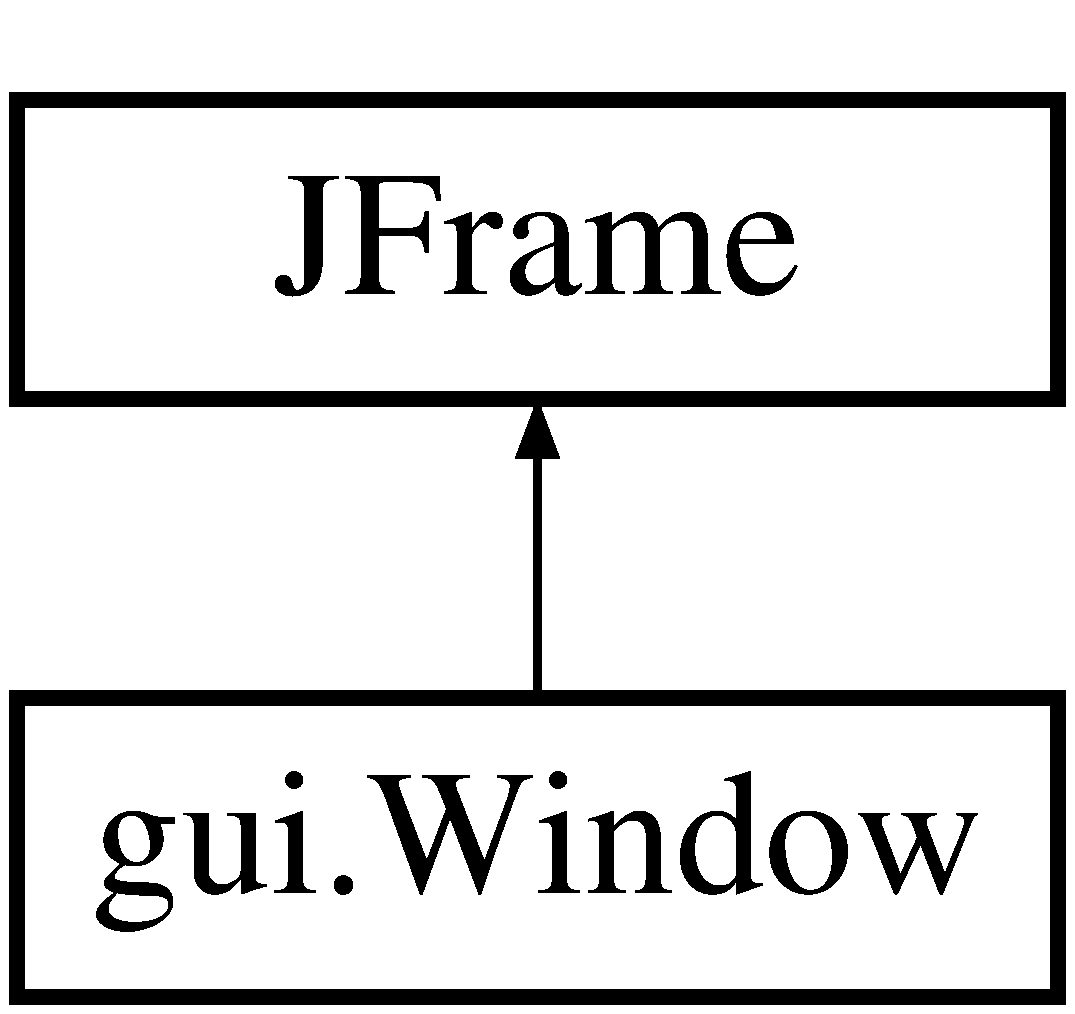
\includegraphics[height=2.000000cm]{classgui_1_1_window}
\end{center}
\end{figure}
\subsection*{Public Member Functions}
\begin{DoxyCompactItemize}
\item 
\mbox{\hyperlink{classgui_1_1_window_a0359cbd3edcac6cc55bf35066661717a}{Window}} (String title, int width, int height)
\item 
Array\+List$<$ \mbox{\hyperlink{classgui_1_1views_1_1_view}{View}} $>$ \mbox{\hyperlink{classgui_1_1_window_aaa2b5dbec79b90c40fca41abb1f99707}{get\+Views}} ()
\end{DoxyCompactItemize}
\subsection*{Static Public Member Functions}
\begin{DoxyCompactItemize}
\item 
static void \mbox{\hyperlink{classgui_1_1_window_af859cb601aa2aca9eab24cc3389fa0e4}{main}} (String\mbox{[}$\,$\mbox{]} args)
\end{DoxyCompactItemize}


\subsection{Constructor \& Destructor Documentation}
\mbox{\Hypertarget{classgui_1_1_window_a0359cbd3edcac6cc55bf35066661717a}\label{classgui_1_1_window_a0359cbd3edcac6cc55bf35066661717a}} 
\index{gui\+::\+Window@{gui\+::\+Window}!Window@{Window}}
\index{Window@{Window}!gui\+::\+Window@{gui\+::\+Window}}
\subsubsection{\texorpdfstring{Window()}{Window()}}
{\footnotesize\ttfamily gui.\+Window.\+Window (\begin{DoxyParamCaption}\item[{String}]{title,  }\item[{int}]{width,  }\item[{int}]{height }\end{DoxyParamCaption})\hspace{0.3cm}{\ttfamily [inline]}}

Make window visible, sets width, height and basic layout options.


\begin{DoxyParams}{Parameters}
{\em title} & -\/ window\textquotesingle{}s title \\
\hline
{\em width} & -\/ window\textquotesingle{}s width in px \\
\hline
{\em height} & -\/ window\textquotesingle{}s height in px \\
\hline
\end{DoxyParams}


\subsection{Member Function Documentation}
\mbox{\Hypertarget{classgui_1_1_window_aaa2b5dbec79b90c40fca41abb1f99707}\label{classgui_1_1_window_aaa2b5dbec79b90c40fca41abb1f99707}} 
\index{gui\+::\+Window@{gui\+::\+Window}!get\+Views@{get\+Views}}
\index{get\+Views@{get\+Views}!gui\+::\+Window@{gui\+::\+Window}}
\subsubsection{\texorpdfstring{get\+Views()}{getViews()}}
{\footnotesize\ttfamily Array\+List$<$\mbox{\hyperlink{classgui_1_1views_1_1_view}{View}}$>$ gui.\+Window.\+get\+Views (\begin{DoxyParamCaption}{ }\end{DoxyParamCaption})\hspace{0.3cm}{\ttfamily [inline]}}

Gets views objects list for avoid duplication of instances \begin{DoxyReturn}{Returns}
array list of views objects 
\end{DoxyReturn}
\mbox{\Hypertarget{classgui_1_1_window_af859cb601aa2aca9eab24cc3389fa0e4}\label{classgui_1_1_window_af859cb601aa2aca9eab24cc3389fa0e4}} 
\index{gui\+::\+Window@{gui\+::\+Window}!main@{main}}
\index{main@{main}!gui\+::\+Window@{gui\+::\+Window}}
\subsubsection{\texorpdfstring{main()}{main()}}
{\footnotesize\ttfamily static void gui.\+Window.\+main (\begin{DoxyParamCaption}\item[{String \mbox{[}$\,$\mbox{]}}]{args }\end{DoxyParamCaption})\hspace{0.3cm}{\ttfamily [inline]}, {\ttfamily [static]}}

Starting point for program, it creates new Thread and object for \mbox{\hyperlink{classgui_1_1_window}{Window}}


\begin{DoxyParams}{Parameters}
{\em args} & -\/ not used \\
\hline
\end{DoxyParams}


The documentation for this class was generated from the following file\+:\begin{DoxyCompactItemize}
\item 
gui/Window.\+java\end{DoxyCompactItemize}

%--- End generated contents ---

% Index
\backmatter
\newpage
\phantomsection
\clearemptydoublepage
\addcontentsline{toc}{chapter}{Index}
\printindex

\end{document}
